% Options for packages loaded elsewhere
\PassOptionsToPackage{unicode}{hyperref}
\PassOptionsToPackage{hyphens}{url}
%
\documentclass[
  Letterpaper,
]{scrbook}

\usepackage{amsmath,amssymb}
\usepackage{iftex}
\ifPDFTeX
  \usepackage[T1]{fontenc}
  \usepackage[utf8]{inputenc}
  \usepackage{textcomp} % provide euro and other symbols
\else % if luatex or xetex
  \usepackage{unicode-math}
  \defaultfontfeatures{Scale=MatchLowercase}
  \defaultfontfeatures[\rmfamily]{Ligatures=TeX,Scale=1}
\fi
\usepackage{lmodern}
\ifPDFTeX\else  
    % xetex/luatex font selection
    \setmainfont[]{Noto Serif CJK SC}
\fi
% Use upquote if available, for straight quotes in verbatim environments
\IfFileExists{upquote.sty}{\usepackage{upquote}}{}
\IfFileExists{microtype.sty}{% use microtype if available
  \usepackage[]{microtype}
  \UseMicrotypeSet[protrusion]{basicmath} % disable protrusion for tt fonts
}{}
\makeatletter
\@ifundefined{KOMAClassName}{% if non-KOMA class
  \IfFileExists{parskip.sty}{%
    \usepackage{parskip}
  }{% else
    \setlength{\parindent}{0pt}
    \setlength{\parskip}{6pt plus 2pt minus 1pt}}
}{% if KOMA class
  \KOMAoptions{parskip=half}}
\makeatother
\usepackage{xcolor}
\usepackage[paperwidth=6in,paperheight=9in]{geometry}
\setlength{\emergencystretch}{3em} % prevent overfull lines
\setcounter{secnumdepth}{5}
% Make \paragraph and \subparagraph free-standing
\makeatletter
\ifx\paragraph\undefined\else
  \let\oldparagraph\paragraph
  \renewcommand{\paragraph}{
    \@ifstar
      \xxxParagraphStar
      \xxxParagraphNoStar
  }
  \newcommand{\xxxParagraphStar}[1]{\oldparagraph*{#1}\mbox{}}
  \newcommand{\xxxParagraphNoStar}[1]{\oldparagraph{#1}\mbox{}}
\fi
\ifx\subparagraph\undefined\else
  \let\oldsubparagraph\subparagraph
  \renewcommand{\subparagraph}{
    \@ifstar
      \xxxSubParagraphStar
      \xxxSubParagraphNoStar
  }
  \newcommand{\xxxSubParagraphStar}[1]{\oldsubparagraph*{#1}\mbox{}}
  \newcommand{\xxxSubParagraphNoStar}[1]{\oldsubparagraph{#1}\mbox{}}
\fi
\makeatother


\providecommand{\tightlist}{%
  \setlength{\itemsep}{0pt}\setlength{\parskip}{0pt}}\usepackage{longtable,booktabs,array}
\usepackage{calc} % for calculating minipage widths
% Correct order of tables after \paragraph or \subparagraph
\usepackage{etoolbox}
\makeatletter
\patchcmd\longtable{\par}{\if@noskipsec\mbox{}\fi\par}{}{}
\makeatother
% Allow footnotes in longtable head/foot
\IfFileExists{footnotehyper.sty}{\usepackage{footnotehyper}}{\usepackage{footnote}}
\makesavenoteenv{longtable}
\usepackage{graphicx}
\makeatletter
\newsavebox\pandoc@box
\newcommand*\pandocbounded[1]{% scales image to fit in text height/width
  \sbox\pandoc@box{#1}%
  \Gscale@div\@tempa{\textheight}{\dimexpr\ht\pandoc@box+\dp\pandoc@box\relax}%
  \Gscale@div\@tempb{\linewidth}{\wd\pandoc@box}%
  \ifdim\@tempb\p@<\@tempa\p@\let\@tempa\@tempb\fi% select the smaller of both
  \ifdim\@tempa\p@<\p@\scalebox{\@tempa}{\usebox\pandoc@box}%
  \else\usebox{\pandoc@box}%
  \fi%
}
% Set default figure placement to htbp
\def\fps@figure{htbp}
\makeatother
% definitions for citeproc citations
\NewDocumentCommand\citeproctext{}{}
\NewDocumentCommand\citeproc{mm}{%
  \begingroup\def\citeproctext{#2}\cite{#1}\endgroup}
\makeatletter
 % allow citations to break across lines
 \let\@cite@ofmt\@firstofone
 % avoid brackets around text for \cite:
 \def\@biblabel#1{}
 \def\@cite#1#2{{#1\if@tempswa , #2\fi}}
\makeatother
\newlength{\cslhangindent}
\setlength{\cslhangindent}{1.5em}
\newlength{\csllabelwidth}
\setlength{\csllabelwidth}{3em}
\newenvironment{CSLReferences}[2] % #1 hanging-indent, #2 entry-spacing
 {\begin{list}{}{%
  \setlength{\itemindent}{0pt}
  \setlength{\leftmargin}{0pt}
  \setlength{\parsep}{0pt}
  % turn on hanging indent if param 1 is 1
  \ifodd #1
   \setlength{\leftmargin}{\cslhangindent}
   \setlength{\itemindent}{-1\cslhangindent}
  \fi
  % set entry spacing
  \setlength{\itemsep}{#2\baselineskip}}}
 {\end{list}}
\usepackage{calc}
\newcommand{\CSLBlock}[1]{\hfill\break\parbox[t]{\linewidth}{\strut\ignorespaces#1\strut}}
\newcommand{\CSLLeftMargin}[1]{\parbox[t]{\csllabelwidth}{\strut#1\strut}}
\newcommand{\CSLRightInline}[1]{\parbox[t]{\linewidth - \csllabelwidth}{\strut#1\strut}}
\newcommand{\CSLIndent}[1]{\hspace{\cslhangindent}#1}

\raggedbottom
\usepackage{xeCJK}
\setCJKmainfont{Noto Serif CJK SC}
\makeatletter
\@ifpackageloaded{tcolorbox}{}{\usepackage[skins,breakable]{tcolorbox}}
\@ifpackageloaded{fontawesome5}{}{\usepackage{fontawesome5}}
\definecolor{quarto-callout-color}{HTML}{909090}
\definecolor{quarto-callout-note-color}{HTML}{0758E5}
\definecolor{quarto-callout-important-color}{HTML}{CC1914}
\definecolor{quarto-callout-warning-color}{HTML}{EB9113}
\definecolor{quarto-callout-tip-color}{HTML}{00A047}
\definecolor{quarto-callout-caution-color}{HTML}{FC5300}
\definecolor{quarto-callout-color-frame}{HTML}{acacac}
\definecolor{quarto-callout-note-color-frame}{HTML}{4582ec}
\definecolor{quarto-callout-important-color-frame}{HTML}{d9534f}
\definecolor{quarto-callout-warning-color-frame}{HTML}{f0ad4e}
\definecolor{quarto-callout-tip-color-frame}{HTML}{02b875}
\definecolor{quarto-callout-caution-color-frame}{HTML}{fd7e14}
\makeatother
\makeatletter
\@ifpackageloaded{bookmark}{}{\usepackage{bookmark}}
\makeatother
\makeatletter
\@ifpackageloaded{caption}{}{\usepackage{caption}}
\AtBeginDocument{%
\ifdefined\contentsname
  \renewcommand*\contentsname{目录}
\else
  \newcommand\contentsname{目录}
\fi
\ifdefined\listfigurename
  \renewcommand*\listfigurename{图索引}
\else
  \newcommand\listfigurename{图索引}
\fi
\ifdefined\listtablename
  \renewcommand*\listtablename{表索引}
\else
  \newcommand\listtablename{表索引}
\fi
\ifdefined\figurename
  \renewcommand*\figurename{图}
\else
  \newcommand\figurename{图}
\fi
\ifdefined\tablename
  \renewcommand*\tablename{表}
\else
  \newcommand\tablename{表}
\fi
}
\@ifpackageloaded{float}{}{\usepackage{float}}
\floatstyle{ruled}
\@ifundefined{c@chapter}{\newfloat{codelisting}{h}{lop}}{\newfloat{codelisting}{h}{lop}[chapter]}
\floatname{codelisting}{列表}
\newcommand*\listoflistings{\listof{codelisting}{列表索引}}
\makeatother
\makeatletter
\makeatother
\makeatletter
\@ifpackageloaded{caption}{}{\usepackage{caption}}
\@ifpackageloaded{subcaption}{}{\usepackage{subcaption}}
\makeatother

\ifLuaTeX
\usepackage[bidi=basic]{babel}
\else
\usepackage[bidi=default]{babel}
\fi
\babelprovide[main,import]{chinese-hans}
\ifPDFTeX
\else
\babelfont{rm}[]{Noto Serif CJK SC}
\fi
% get rid of language-specific shorthands (see #6817):
\let\LanguageShortHands\languageshorthands
\def\languageshorthands#1{}
\usepackage{bookmark}

\IfFileExists{xurl.sty}{\usepackage{xurl}}{} % add URL line breaks if available
\urlstyle{same} % disable monospaced font for URLs
\hypersetup{
  pdftitle={Eyes on Health},
  pdfauthor={Richard Sprague},
  pdflang={zh-Hans},
  hidelinks,
  pdfcreator={LaTeX via pandoc}}


\title{Eyes on Health}
\author{Richard Sprague}
\date{2025-03-23}

\begin{document}
\frontmatter
\maketitle

\renewcommand*\contentsname{目录}
{
\setcounter{tocdepth}{1}
\tableofcontents
}

\mainmatter
\bookmarksetup{startatroot}

\chapter*{前言}\label{ux524dux8a00}
\addcontentsline{toc}{chapter}{前言}

\markboth{前言}{前言}

人类的眼睛长期以来吸引着医学专业人士,成为了解整体健康状况的独特窗口。通过视网膜的精细结构,我们可以观察到错综复杂的血管网络、神经组织和代谢活动------所有这些都无需任何切口或侵入性操作。这一非凡的观察点使视网膜成像技术,尤其是眼底摄影,成为健康评估和预防保健中日益重要的工具。

高分辨率成像技术与人工智能的融合彻底改变了我们收集和解释视网膜数据的能力。曾经仅限于眼科医生领域的技术现在已经为更广泛的健康专业人士所用,为早期发现和监测各种系统性疾病开辟了新的可能性。

本书探讨了眼底摄影在临床实践中的科学原理、应用和未来潜力,特别关注Opticare
AI相机系统。我们将研究将视网膜标志物与各种健康状况相关联的大量研究,从心血管疾病到认知能力下降。同时,我们将保持客观视角,探讨当前技术能做什么和不能做什么,帮助从业者设定适当的期望,并做出明智的决定,将这项技术整合到他们的实践中。

对于健康专业人士------无论您是自然疗法医师、脊椎按摩师、营养师还是医生------本书提供了关于眼底摄影如何补充您现有实践的见解。我们将探讨这项技术如何增强患者参与度,提供有价值的健康见解,并与其他诊断工具结合,实现更全面的健康管理方法。

通过科学证据、实用指导和对健康诊断未来的前瞻性观点,我们的目标是为您提供必要的知识,以便在将眼底摄影技术纳入实践时做出明智的决定,同时激发您对预防性健康评估未来的广泛思考。无论您对视网膜摄影了解多少,都将对眼睛作为人类健康窗口的角色和现代成像技术的变革潜力有更深入的认识。

要了解更多关于Opticare的信息,请访问 \url{https://opticare.ai}。

\pagebreak

\begin{tcolorbox}[enhanced jigsaw, coltitle=black, rightrule=.15mm, colback=white, colbacktitle=quarto-callout-caution-color!10!white, breakable, bottomtitle=1mm, opacityback=0, bottomrule=.15mm, titlerule=0mm, opacitybacktitle=0.6, left=2mm, colframe=quarto-callout-caution-color-frame, title=\textcolor{quarto-callout-caution-color}{\faFire}\hspace{0.5em}{免责声明}, toptitle=1mm, toprule=.15mm, arc=.35mm, leftrule=.75mm]

本书提供的信息仅供教育和参考之用。它不构成医疗建议、诊断或治疗。Opticare
AI系统目前未获得FDA授权用于诊断或治疗任何疾病。在做出任何关于您的健康的决定或将新技术纳入您的实践之前,请始终咨询合格的医疗专业人士。作者和出版商对因使用或应用本书中包含的任何信息而直接或间接产生的任何责任概不负责。虽然我们已尽力确保所呈现信息的准确性,但医疗实践、法规和技术不断发展,读者应独立验证当前信息。对特定研究研究、技术和应用的引用仅提供背景,不应被视为对功效或结果的认可或保证。

\end{tcolorbox}

\bookmarksetup{startatroot}

\chapter{眼睛作为窗口:揭示视网膜成像的力量}\label{ux773cux775bux4f5cux4e3aux7a97ux53e3ux63edux793aux89c6ux7f51ux819cux6210ux50cfux7684ux529bux91cf}

\section{引言:眼见为实的背后}\label{ux5f15ux8a00ux773cux89c1ux4e3aux5b9eux7684ux80ccux540e}

人类的眼睛,这个复杂的视觉感知器官,常常因其感知周围世界的能力而受到赞美。然而,这个非凡的器官拥有远超视觉功能的潜力。它是一个复杂的、活生生的组织------人体的一个微观世界,具有独特的血管和神经结构,为我们提供了一个直接、非侵入性的窗口来了解一个人的整体健康状况。当我们深入研究现代成像技术,特别是眼底摄影的能力时,我们开始揭示医学中的一个新范式,眼睛作为一种强大的诊断工具,远远超出了传统眼科学的范畴。

几个世纪以来,视网膜的检查仅限于使用传统检眼镜所能观察到的内容。虽然这仍然是一种有价值的技术,但检眼镜检查需要专业培训、熟练的眼力,而且无法以易于存储或共享的方式捕捉信息\footnote{Lin
  等 (2021)}。然而,现代技术带来了非散瞳眼底相机,当与人工智能结合时,释放了视网膜成像的隐藏潜力。借助这些进步,视网膜血管和眼睛其他结构中可见的微妙变化现在可以被量化并与广泛的全身性疾病相关联,从而改变了我们对健康评估的方式。这种通过单一、相对简单、非侵入性程序看到的身体新视野,有潜力彻底改变我们对诊断医学、预防性护理和更个性化健康管理的方法。

在本书中,我们将踏上探索这一激动人心前沿领域的旅程。我们将研究支持使用视网膜眼底成像评估一般健康状况的新兴科学证据,这些发现如何转化为临床或健康环境,最后我们将探讨这一新兴领域的未来方向,以及Opticare如何引领这一变革。到本书结束时,你将理解诗人威廉·布莱克的话:``眼睛所见远超心所知。''

\section{视网膜:身体的独特微观世界}\label{ux89c6ux7f51ux819cux8eabux4f53ux7684ux72ecux7279ux5faeux89c2ux4e16ux754c}

位于眼球后部的视网膜不仅仅是一种感光组织;它是大脑的非凡延伸。它在胚胎发育过程中的形成与中枢神经系统密切相关。视网膜和大脑都在胚胎发生过程中来源于神经管,这导致了共享的生物学途径和共同的细胞类型。这种密切联系意味着视网膜不仅仅是视觉信息的被动接收者,而是中枢神经系统的活跃延伸,因此可以反映身体的整体神经健康状况。

当医疗专业人员检查眼睛时,他们观察的是''眼底''------位于晶状体对面的眼睛内部表面,包括视网膜、视盘、黄斑和后极。``眼底''一词来源于拉丁语,意为''底部''或''基部'',因为它代表了在检查过程中可以可视化的眼睛内部后部分。当我们在本书中提到眼底摄影或成像时,我们讨论的是对眼睛内部后表面的专业摄影,其中包含反映眼部和全身健康的这些关键结构。

\begin{figure}[H]

{\centering \pandocbounded{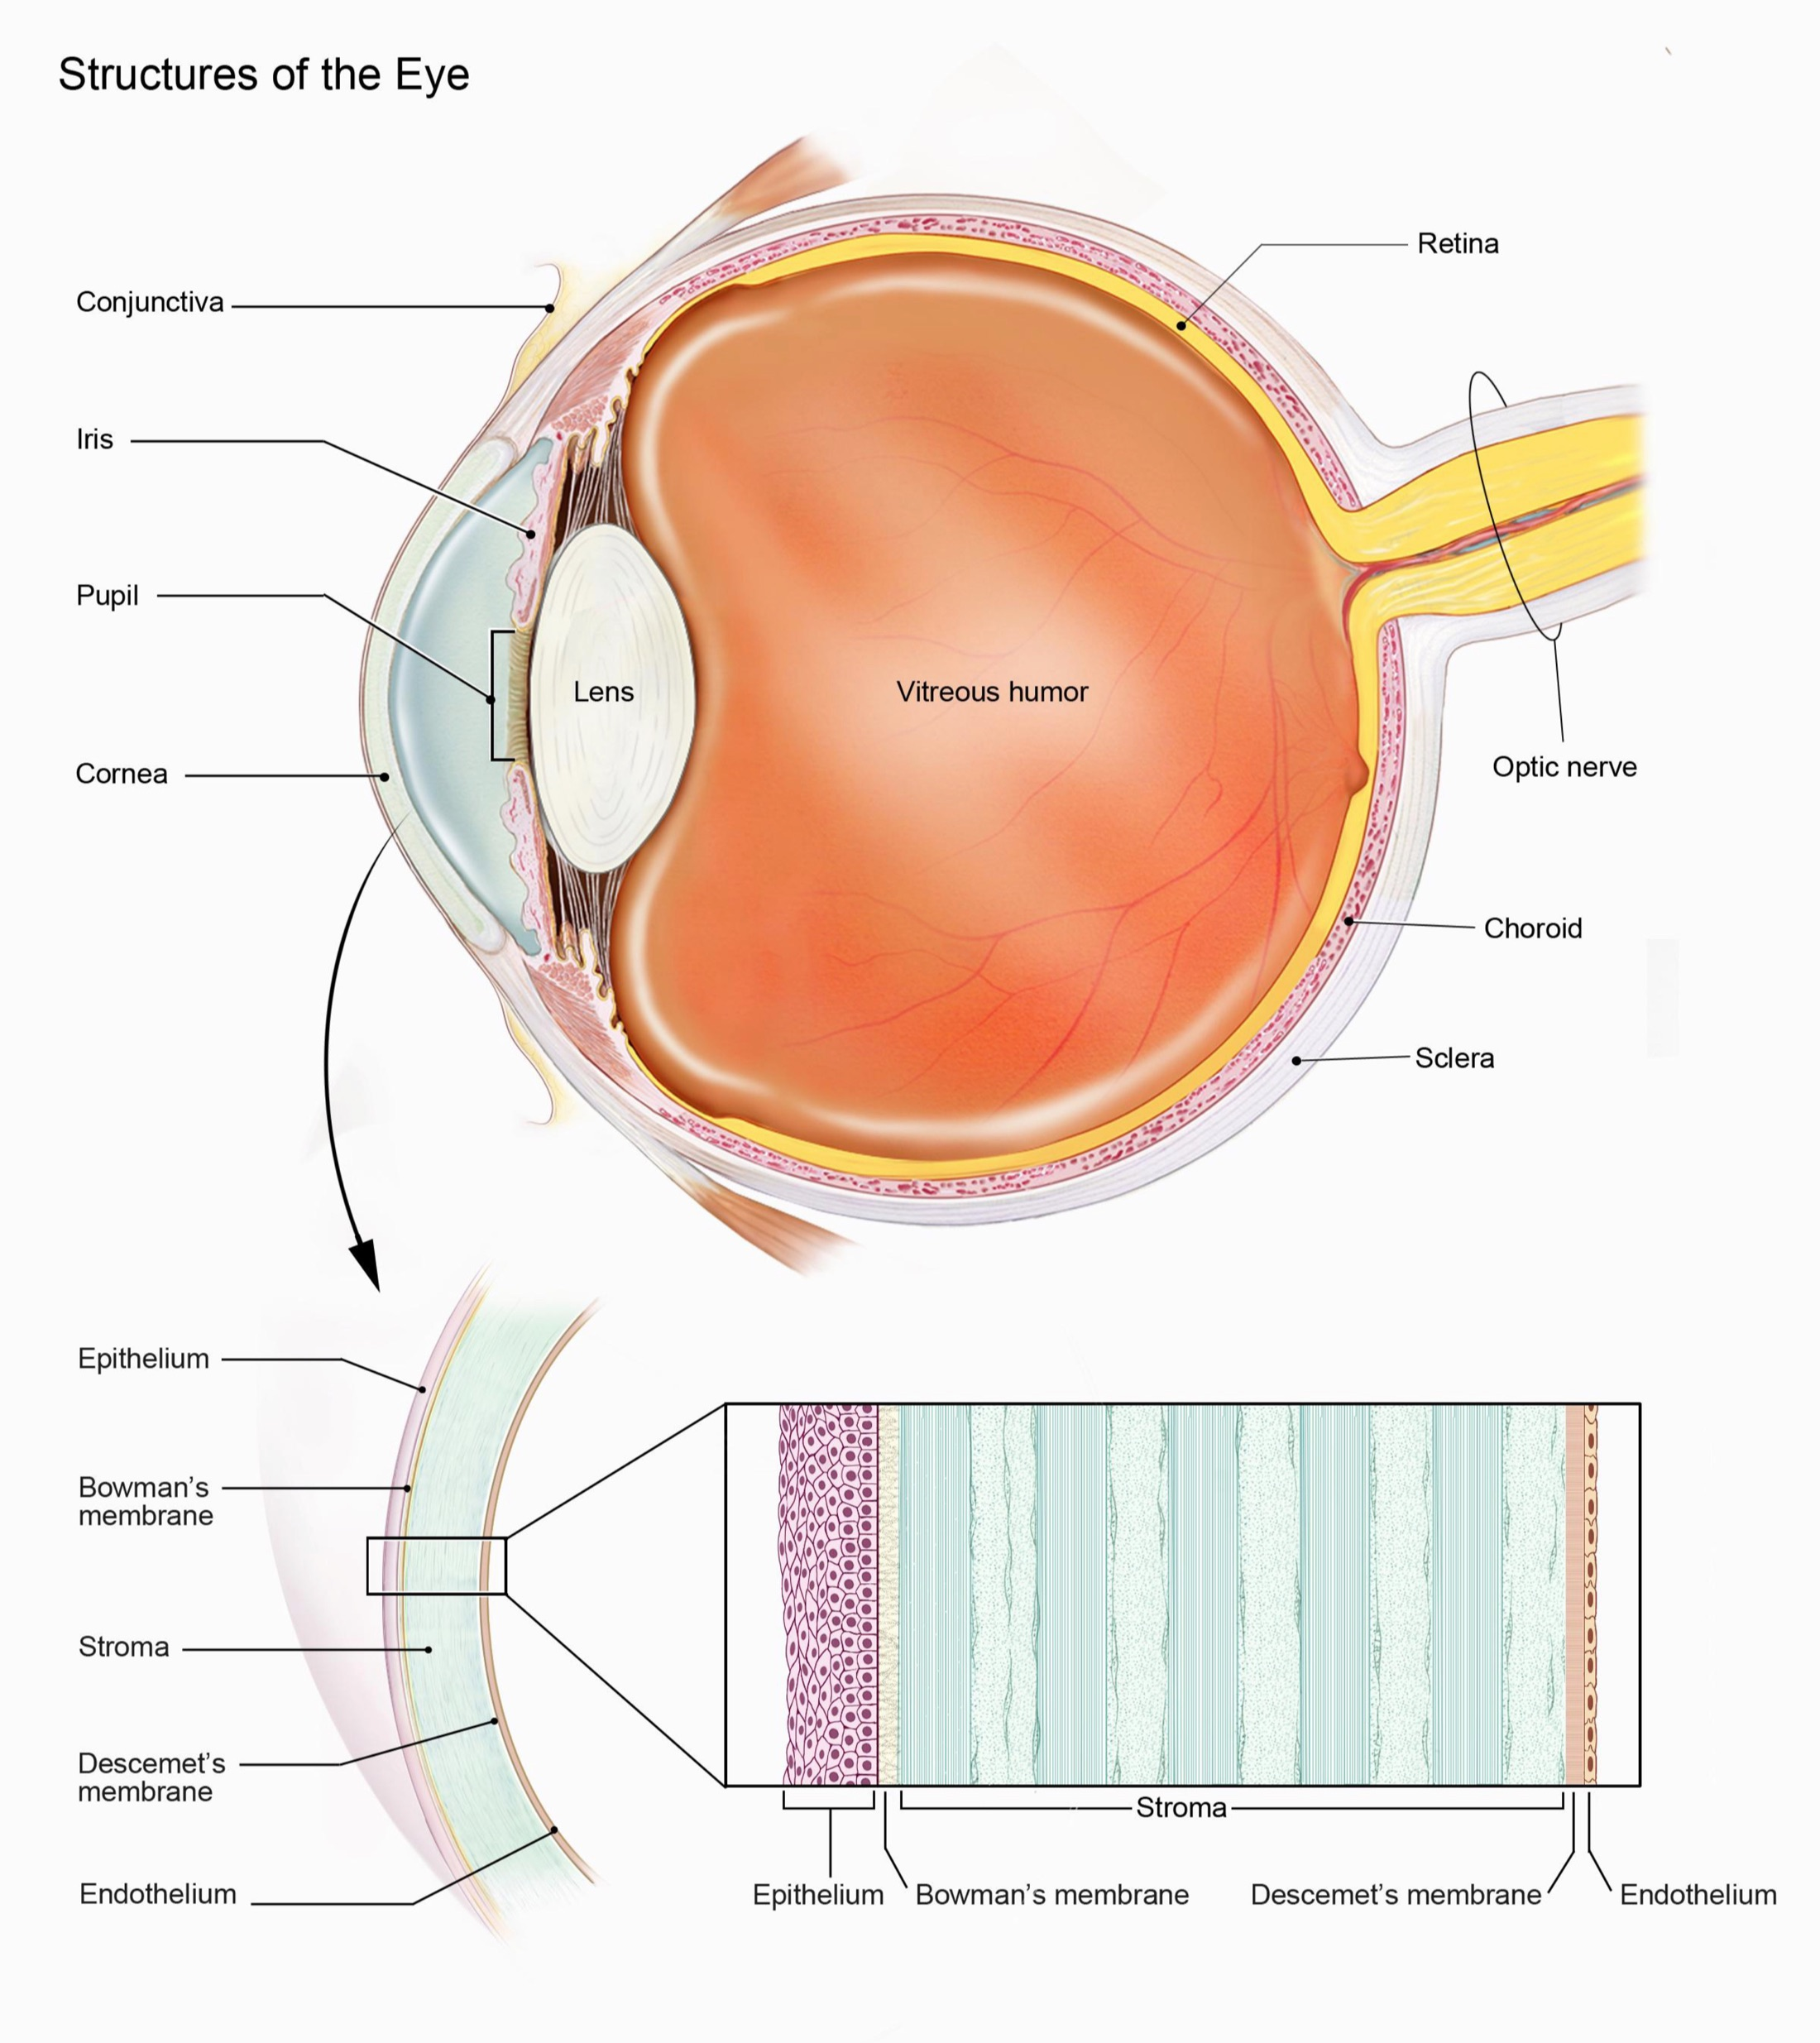
\includegraphics[keepaspectratio]{_resources/images/ch1/Structures-of-the-eye.jpg}}

}

\caption{眼睛结构(来源:\href{https://medialibrary.nei.nih.gov/}{美国国家眼科研究所})}

\end{figure}%

从结构上看,视网膜是一个多层膜,包含感光细胞、中间神经元、神经节细胞和胶质细胞。这些神经元负责将光信号转换为电脉冲,然后发送到大脑进行处理。但对于本次讨论而言,也许更重要的是,视网膜拥有精细且高度血管化的微血管网络。视网膜微血管系统由小动脉、毛细血管和小静脉组成,促进了营养物质和氧气的输送,这对视网膜细胞的高代谢活动至关重要,同时也清除代谢废物。视网膜微血管系统可通过眼底摄影等非侵入性方法高度可及。这种血管系统在结构上是独特的。与其他血管相比,视网膜血管清晰可见且可直接观察,不被组织或皮肤遮蔽,使其成为研究微血管功能障碍的完美模型。视网膜小动脉和小静脉对生理变化也非常敏感,鉴于它们是较大循环系统的一部分,也可以反映其他器官的病理过程。

\begin{figure}[H]

{\centering \pandocbounded{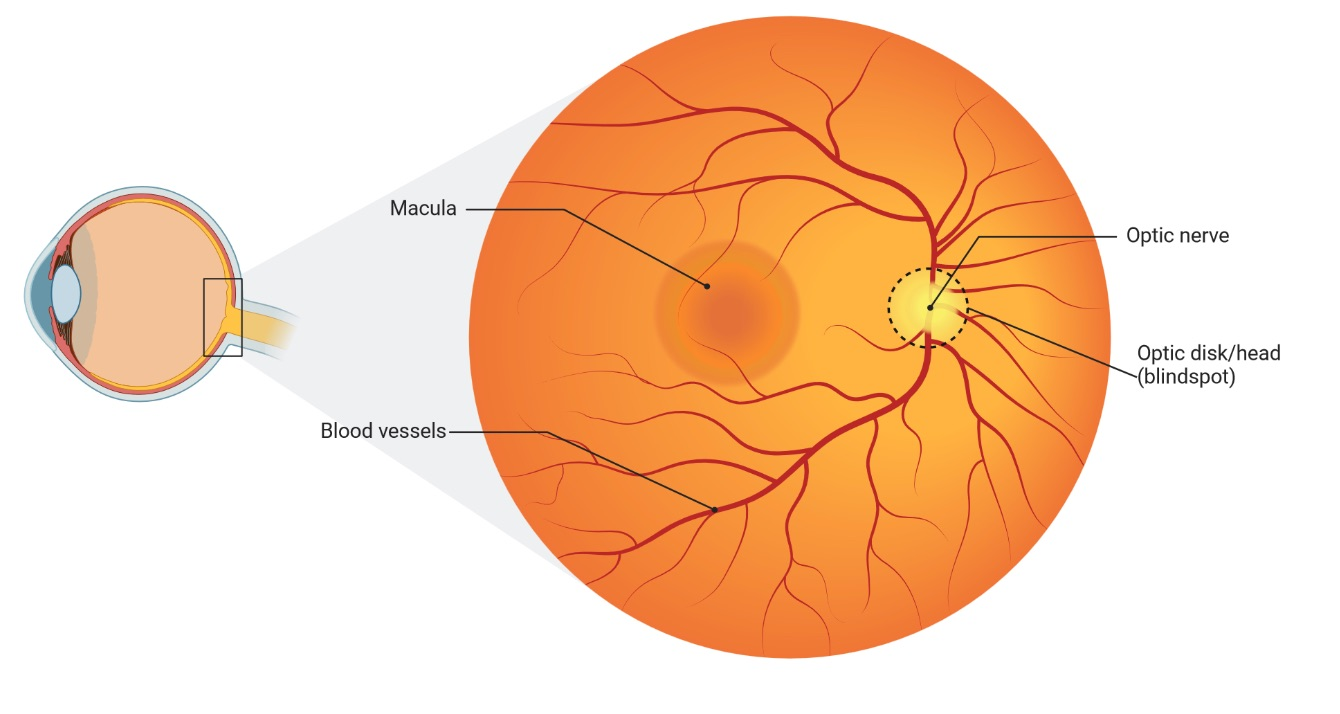
\includegraphics[keepaspectratio]{_resources/images/BioRenderFundusHumanEye.jpg}}

}

\caption{人眼眼底(来源:\href{https://app.biorender.com/biorender-templates/t-66a629a6675d6a46372e7cb4}{Biorender})}

\end{figure}%

此外,视网膜和脉络膜是高耗氧组织,因此当氧气供应或代谢废物清除受损时,其细胞对细胞损伤的敏感性很高。因此,许多研究人员发现视网膜结构与各种全身性疾病之间存在联系并不令人惊讶。视网膜血液供应与其他神经组织的紧密整合也使其成为研究糖尿病、高血压、心脏病和神经退行性疾病等全身性疾病影响的理想场所。总而言之,视网膜的独特特性------与大脑的直接联系、高度可见的微血管系统和高代谢活动------使其成为评估整体全身健康的强大非侵入性工具。

\section{常见眼部病理:通过眼底观察}\label{ux5e38ux89c1ux773cux90e8ux75c5ux7406ux901aux8fc7ux773cux5e95ux89c2ux5bdf}

虽然本书主要关注视网膜成像用于评估全身健康的应用,但了解通过眼底摄影容易观察到的常见眼部病理也很重要。这些情况虽然传统上由眼科医生评估,但在审查视网膜图像时了解它们很重要。了解这些眼部疾病可以帮助临床医生理解何时进行转诊,并有助于说明使用视网膜进行健康评估和诊断的重要性。在此,我们将探讨几种最常见的可通过眼底成像检测到的眼部疾病:

\textbf{糖尿病视网膜病变 (DR):}
糖尿病视网膜病变是糖尿病的微血管并发症,也是全球致盲的主要原因之一。它发生在高血糖水平损害视网膜中的小血管时,导致一系列病理变化。DR的最早迹象包括微动脉瘤(毛细血管的小扩张)、出血(受损血管渗血)和渗出物(渗漏血管中的液体和蛋白质沉积物)。这些变化进展为更严重的疾病形式,如增殖性糖尿病视网膜病变,可能包括新生血管形成。糖尿病视网膜病变的视网膜变化在疾病早期阶段通常很微妙,因此容易被传统方法忽视。

眼底摄影对于糖尿病视网膜病变的早期检测至关重要。早期检测至关重要,因为DR在初始阶段是高度可治疗的。治疗选择始于改善血糖控制和血压管理,但随着病情进展通常需要特定的眼科干预。

对于更高级的病例,治疗包括激光光凝,这是一种相对快速的门诊手术,使用激光密封渗漏血管并防止新的异常血管形成。这种20-30分钟的手术在局部麻醉下进行,患者通常第二天就能恢复正常活动,尽管可能需要多次治疗。

另一种治疗选择是抗VEGF(血管内皮生长因子)疗法。VEGF是一种刺激新血管生长的蛋白质,在糖尿病视网膜病变中,这些血管可能很脆弱且容易渗漏。抗VEGF药物如雷珠单抗(Lucentis)或阿柏西普(Eylea)直接注射到眼内以阻断这种蛋白质,减少异常血管生长和液体渗漏。这些注射在眼科医生办公室进行,局部麻醉下只需几分钟,尽管为达到最佳效果可能需要每4-6周重复一次。

对于更严重的病例,可能需要玻璃体切除手术。这是在医院环境中进行的更具侵入性的手术,将眼睛的玻璃体凝胶去除,以便修复视网膜。玻璃体切除手术的恢复通常需要几周时间,可能需要限制体位和活动。

如果不及时干预,DR可能会发展为严重的视力损害或失明,可能是不可逆的。此外,治疗晚期DR的成本比早期干预要高得多,无论是在经济上还是在患者生活质量方面。

通过眼底摄影可视化的变化通常具有诊断意义,可以启动生活方式改变和其他治疗干预,防止糖尿病视网膜病变和视力丧失的进展。DR的早期识别也可能是更广泛的全身血管变化的指标,并强调了更好地管理糖尿病全身疾病的需要。

\begin{figure}[H]

{\centering 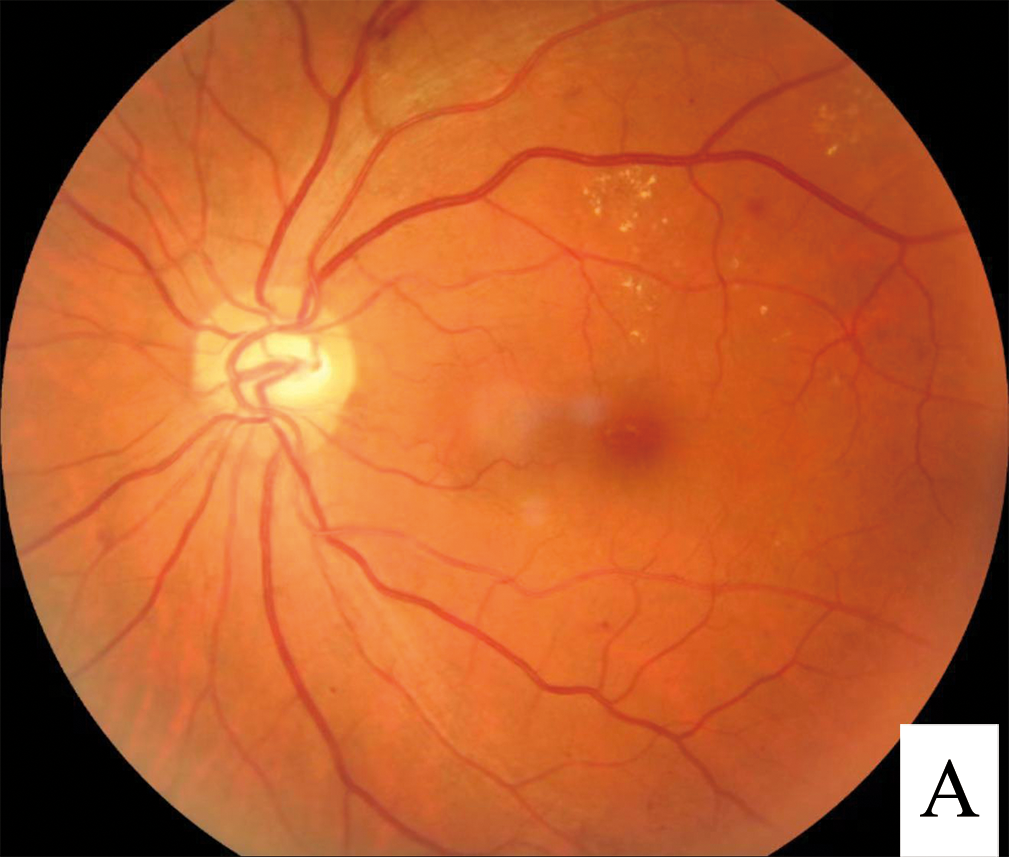
\includegraphics[width=3.64583in,height=\textheight,keepaspectratio]{_resources/images/pathologies/Fundus_-_diabetic_retinopathy.png}

}

\caption{眼底图像显示多种糖尿病视网膜病变征象:硬性渗出物(散布的黄色斑点)、微动脉瘤(一些血管上的突起)和小出血(模糊的红点)。\\
来源:\href{https://en.wikipedia.org/wiki/Diabetic_retinopathy}{维基百科}}

\end{figure}%

\textbf{年龄相关性黄斑变性 (AMD):}
年龄相关性黄斑变性是一种影响黄斑的进行性疾病,黄斑是负责中央视力的视网膜部分。AMD是老年人群视力丧失的主要原因之一。AMD的发病机制很复杂,环境、遗传、代谢和免疫因素都起着重要作用。AMD有两种主要类型:干性和湿性。在干性AMD中,玻璃膜疣(黄色沉积物)形成于视网膜和RPE下方,可能导致黄斑萎缩。在湿性AMD中,异常血管在视网膜下生长,导致渗漏和出血,因此导致视力快速下降。

两种AMD形式的治疗选择差异很大。对于占病例约85-90\%的干性AMD,目前没有FDA批准的可以逆转这种情况的治疗方法。然而,大型临床试验表明,特定高剂量营养补充剂(称为AREDS2配方,含有维生素C和E、锌、铜、叶黄素和玉米黄素)可在五年内将进展至晚期的风险降低约25\%。生活方式修改,包括戒烟、定期锻炼、维持正常血压和食用富含绿叶蔬菜和鱼类的饮食,也可能有助于减缓进展。

对于湿性AMD,治疗选择更具干预性和时间敏感性。标准护理包括类似于糖尿病视网膜病变使用的抗VEGF注射。这些药物(包括雷珠单抗(Lucentis)、阿柏西普(Eylea)和贝伐单抗(Avastin))最初通常每四到八周直接注射到眼内一次。这些门诊手术仅需几分钟,在局部麻醉下进行。较新的制剂如布洛芦单抗(Beovu)可能允许减少注射频率。及时给药时,这些注射可以稳定90\%以上患者的视力,并改善约三分之一病例的视力。

对于不响应抗VEGF治疗的患者,可以考虑光动力疗法。这种两步门诊手术包括静脉内给予对光敏感的药物,该药物在异常血管中浓缩,然后应用冷激光激活药物并密封渗漏血管。

眼底摄影是早期检测AMD的关键工具,使临床医生能够识别玻璃膜疣或黄斑中的其他微妙变化。视网膜下玻璃膜疣(黄色沉积物)的存在和黄斑中的色素变化也可以指示疾病的早期阶段,提供预防行动的机会。眼底照片的AI分析可以实现AMD的早期检测和分类,这可能导致早期干预,如生活方式修改和维生素补充,可能减缓疾病的进展。它还允许快速识别AMD的湿性形式,这种形式更严重,新发湿性AMD患者会紧急转诊给视网膜专家进行干预。鉴于湿性AMD的有效治疗窗口很窄------通常以天而非周计------这种快速识别可以挽救视力。

\begin{figure}[H]

{\centering 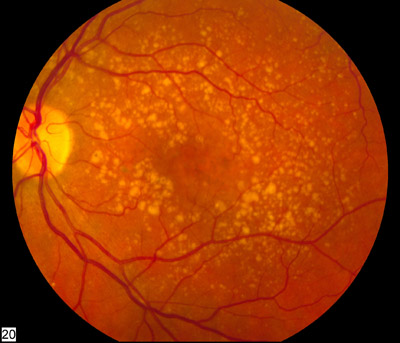
\includegraphics[width=3.64583in,height=\textheight,keepaspectratio]{_resources/images/pathologies/Intermediate_age_related_macular_degeneration.jpg}

}

\caption{年龄相关性黄斑变性
(AMD):注意图像中散布的黄色沉积物(玻璃膜疣)。\\
来源:\href{https://commons.wikimedia.org/wiki/File:Intermediate_age_related_macular_degeneration.jpg}{维基百科}}

\end{figure}%

\textbf{青光眼性视神经病变:}
青光眼是一组进行性视神经疾病,特征是视网膜神经节细胞死亡和随之而来的视野丧失。虽然最常与眼内压升高相关,但青光眼也可能发生在眼压正常或低的人群中。青光眼的发病机制被认为包括眼内压增加导致视盘和视网膜神经纤维层的机械应力以及神经头部血液供应受损。

虽然确定性青光眼诊断通常需要综合评估,包括测眼压、视野测试,以及通常使用光学相干断层扫描(OCT)测量视网膜神经纤维层厚度,但眼底摄影在青光眼评估中仍然发挥重要作用。视神经头是评估青光眼时评估的主要结构之一,对这一结构的变化可以在眼底照片中初步观察到。在青光眼中,视神经可能看起来更大,显示杯形扩大或视盘周围组织边缘的丧失。

视网膜眼底成像作为重要的筛查和监测工具,可能识别需要更确定性测试的患者。它还可用于记录基线视神经外观并随时间追踪结构变化。AI算法可以帮助标准化从眼底图像评估视神经头参数,如盘杯比、神经视网膜缘面积和血管外观,这可能提高筛查效率并支持临床决策。然而,重要的是要注意,这些发现应与其他临床测量相关联,以便制定确定性的青光眼诊断和管理计划。

\textbf{高血压性视网膜病变 (HPR):}
高血压性视网膜病变是另一种与高血压高度相关的微血管疾病,其特征是由高血压引起的视网膜血管损伤。视网膜变化的严重程度通常与高血压的严重程度和持续时间相关。HPR在眼底照片上的临床表现包括视网膜小动脉变窄、小静脉压迫、动静脉交叉改变以及由于血管渗漏引起的出血或渗出物。在更高级阶段,患者还可能出现棉絮斑(视网膜神经纤维层缺血区域)。视网膜成像是检测和监测高血压性视网膜病变的重要工具,因为它可以提供高血压导致微血管损伤的早期指征。AI驱动的分析可以帮助诊断HPR,这可能表明患者在见到内科或心血管专家之前就需要管理高血压,从而导致更好的长期健康结果。

\textbf{视盘玻璃膜疣:}
视盘玻璃膜疣是视神经头中的异常蛋白质和钙沉积物。它们通常是良性状况,但在一些罕见情况下,如果它们扩大或导致神经纤维压缩,可能导致视力丧失。玻璃膜疣是眼底成像中的常见发现,通常具有白色、黄色或透明质的外观,边界清晰,有助于临床医生确定病变的性质。由于玻璃膜疣有时可能模仿视盘水肿的外观,准确识别视盘玻璃膜疣对于正确诊断很重要。视盘玻璃膜疣最容易用无红光照明可视化。AI可以量化玻璃膜疣的大小、形状和数量,用于长期监测,这有助于这些患者的整体管理。

\textbf{视网膜静脉阻塞 (RVO):}
视网膜静脉阻塞发生在视网膜血管被阻塞时,可能导致突然视力丧失。RVO与心血管疾病和糖尿病等潜在全身性疾病相关。RVO的两种常见类型是分支视网膜静脉阻塞(BRVO)和中央视网膜静脉阻塞(CRVO),基于阻塞的位置。眼底照片上的临床发现包括视网膜出血、棉絮斑、视网膜小静脉扩张和视网膜水肿。具有AI算法的视网膜成像可用于检测和监测RVO的严重程度,并帮助诊断与这些情况相关的潜在全身性疾病。

\section{传统检眼镜检查:局限性和新视角}\label{ux4f20ux7edfux68c0ux773cux955cux68c0ux67e5ux5c40ux9650ux6027ux548cux65b0ux89c6ux89d2}

150多年来,检眼镜检查,即使用检眼镜直接检查视网膜,一直是诊断和管理眼部疾病的基本工具。这种技术在19世纪中期发展起来,允许临床医生通过向瞳孔照射光线来可视化视盘、视网膜和视网膜血管。传统检眼镜检查历来用于评估糖尿病视网膜病变、年龄相关性黄斑变性、青光眼和其他眼部疾病等视网膜疾病。虽然它提供了视网膜的直接视图,但随着技术的发展,这种技术的几个局限性变得更加明显。

传统检眼镜检查的主要局限性之一是需要高度的技能和培训才能准确解释发现。学习曲线以变得精通于解释所见内容是相当陡峭的,观察者间的变异性可能相当高。这是由于可视化质量的变异性以及在分析视网膜复杂模式时主观性的介入。临床医生,尤其是非眼科医生,往往无法完全理解可能表明早期或潜在病理的微妙变化。此外,可视化本质上受到观察者视野和保持焦点能力的限制。这些限制还妨碍了检眼镜检查作为人口健康筛查工具的使用,因为需要高技能的提供者并且难以获得一致的结果。

传统检眼镜检查的另一个重要局限性是其无法数字捕获和存储视网膜图像以供进一步分析或审查。检眼镜检查只提供短暂的可视化,没有记录或数字存档的发现,这意味着随时间的变化或微妙的异常可能难以跟踪。此外,难以与其他临床医生分享图像以进行咨询和第二意见。这种永久记录的缺乏降低了传统检眼镜检查的整体临床价值。

传统检眼镜检查的这些缺点导致人们对眼底摄影,特别是不需要瞳孔扩张的非散瞳相机,作为评估视网膜的更可及、高效和可靠的方式产生了浓厚的兴趣。与传统检眼镜检查相比,非散瞳眼底相机利用数字传感器和专门的光学系统捕捉视网膜的高分辨率图像,无需扩张瞳孔。这意味着非眼科医生可以获取视网膜图像,只需最少的培训,然后可以远程共享数据或将图像整合到电子病历中。通过能够捕获永久数字记录,图像可以存档并共享以供审查和咨询。这种能力在需要追踪视网膜结构随时间变化的纵向研究中尤为重要。当与AI算法结合使用时,视网膜图像成为一种非常强大的工具,可以评估各种疾病和健康状况,超越了仅仅眼睛疾病的范畴。

\section{眼底摄影}\label{ux773cux5e95ux6444ux5f71}

非散瞳眼底摄影的出现代表了我们评估视网膜,进而评估患者整体健康能力的一大飞跃。这种技术采用数字相机和专门的光学系统,无需使用扩瞳眼药水即可捕捉视网膜(眼球后部的感光组织)的详细、高分辨率图像。这种非侵入性方法开启了大规模视网膜筛查的可能性,这在传统检眼镜检查中是不可行的。这种技术快速、方便并提供了可能与各种利益相关者共享(包括专家)或存储以供后续分析的数据访问。

眼底摄影背后的技术很简单:光源照亮视网膜,反射的图像被高分辨率数字传感器捕获。大多数现代眼底相机都有先进的光学系统,减少眩光和失真,从而产生视网膜血管、视盘、黄斑和其他结构的异常清晰图像。这些图像提供了视网膜结构(包括微血管系统)的广泛概览,然后可以进行数字评估,发现任何可能对肉眼不明显的微妙变化。图像获取的便捷性也有助于促进远程视网膜服务的发展,远程地区的训练有素的人员能够使用相机并与远程临床医生共享数据。此外,自动化数据分析可用于提取和量化有关视网膜结构和微血管系统的信息,为以前不可能实现的大规模筛查铺平了道路。

\section{杯盘比:眼部健康的窗口}\label{ux676fux76d8ux6bd4ux773cux90e8ux5065ux5eb7ux7684ux7a97ux53e3}

杯盘比(CDR)代表了视网膜评估中最重要的测量之一,特别是用于评估视神经健康和筛查青光眼。这一测量,可以通过眼底摄影准确确定,提供了对视神经头结构完整性的关键洞察。

\textbf{了解解剖结构}

视盘,也称为视神经头,是视网膜神经纤维离开眼睛形成视神经的点。通过眼底摄影观察时,视盘呈现为大致圆形区域,通常显示粉红色或橙黄色。在这个视盘内,有两个明显的区域:

\begin{enumerate}
\def\labelenumi{\arabic{enumi}.}
\tightlist
\item
  \textbf{神经视网膜缘}:视盘的外部分,包含神经纤维束
\item
  \textbf{杯部}:血管进入和离开眼睛的中央凹陷
\end{enumerate}

杯盘比比较杯部直径与视盘总直径的比例。在健康的眼睛中,杯部通常占整个视盘直径的不到一半,导致CDR小于0.5。然而,健康个体之间存在相当大的变异,被认为''正常''的范围可以从0.1到0.4不等。

\textbf{临床意义}

CDR作为视神经健康的关键指标,原因有几个:

\begin{enumerate}
\def\labelenumi{\arabic{enumi}.}
\tightlist
\item
  \textbf{青光眼检测}:杯部相对于视盘的进行性扩大(CDR增加)通常表明青光眼性损伤。随着眼内压升高损害神经纤维,杯部以神经视网膜缘为代价扩大。
\item
  \textbf{纵向监测}:定期测量CDR允许医生追踪随时间的变化。一个稳定的比率,即使大于平均值,可能比显示进行性增加的比率更不令人担忧。
\item
  \textbf{风险评估}:研究表明,较大的基线CDR可能表明发展为青光眼的风险增加,特别是当与眼内压升高或家族史等其他风险因素结合时。
\end{enumerate}

\textbf{通过技术测量}

具有AI功能的现代眼底相机可以自动计算CDR,具有高精度。这代表了传统手动评估方法的显著进步:

\begin{itemize}
\tightlist
\item
  一致性:自动测量消除了观察者间的变异性
\item
  精确性:数字分析可以检测可能逃过人类观察的微妙变化
\item
  文档记录:数字记录使精确追踪随时间的变化成为可能
\item
  效率:快速自动分析节省医生时间,同时保持准确性
\end{itemize}

虽然CDR提供了有价值的信息,但应始终在更广泛的临床背景下解释:

\begin{enumerate}
\def\labelenumi{\arabic{enumi}.}
\tightlist
\item
  \textbf{个体差异}:正常CDR在不同人群和个体间有所不同。视盘大小和种族等因素可能影响什么被认为是正常的。
\item
  \textbf{不对称性}:患者双眼之间的CDR差异(大于0.2)可能表明病理状况,即使单独测量值在正常范围内。
\item
  \textbf{模式识别}:杯部扩大的模式很重要。杯部垂直延长通常比水平扩大更能暗示早期青光眼变化。
\item
  \textbf{互补措施}:CDR应与其他临床发现一起考虑,包括眼内压、视野测试和整体视网膜健康。
\end{enumerate}

对于健康专业人士,通过眼底摄影进行自动CDR测量提供了几个优势:

\begin{enumerate}
\def\labelenumi{\arabic{enumi}.}
\tightlist
\item
  早期检测:在发生显著视力丧失之前识别令人担忧的变化
\item
  客观监测:精确追踪随时间的变化
\item
  客户教育:视觉展示视神经健康状态
\item
  风险分层:更好地识别需要专业眼科护理的客户
\end{enumerate}

了解CDR解释使从业者能够对客户护理和转诊模式做出更明智的决定。虽然单独不具诊断性,但CDR代表了通过视网膜成像进行全面健康评估的有价值组成部分。

请记住,虽然自动CDR测量提供了有价值的洞察力,但它应该始终被视为全面健康评估的一个组成部分。CDR的变化应在指示时促使适当转诊给眼科专家进行详细评估。

\section{超越眼睛的视野}\label{ux8d85ux8d8aux773cux775bux7684ux89c6ux91ce}

高分辨率眼底摄影的益处通过人工智能的近期进步得到了进一步提升。通过将眼底照片与AI结合,新的分析参数成为可能。深度学习方法可以精确计算血管直径并检测视网膜结构中的微小变化,这对于一个熟练的眼科医生来说需要更长时间才能评估。AI算法正在迅速完善,它们分析视网膜图像以发现心脏病、糖尿病和神经系统疾病等全身性疾病迹象的能力很有前途。随着我们在本书中继续探索,我们将进一步探讨AI如何实现对视网膜健康及其与全身疾病联系的更细微理解,以及将这些系统整合到当前临床实践和研究计划中的潜力。

\bookmarksetup{startatroot}

\chapter{科学基础:证据揭示了什么}\label{ux79d1ux5b66ux57faux7840ux8bc1ux636eux63edux793aux4e86ux4ec0ux4e48}

在第一章中,我们探讨了视网膜如何成为人类健康的一个非凡窗口。我们讨论了它独特的解剖和生理特性,它与大脑的联系,以及通过传统眼底摄影可见的各种眼部病理学。本章迈出了下一步------探讨人工智能如何将视网膜成像从专业诊断工具转变为全面健康评估的强大平台。

几十年来,视网膜评估受到人类感知能力的限制。即使是受过高度训练的眼科医生也受到人眼能辨别和人脑能处理的内容的限制。微妙的血管变化、微小的组织变化和复杂的模式关系往往保持不可见或无法识别。人工智能的引入从根本上改变了这一范式。

传统诊断依赖于识别已知的病理特征------青光眼的扩大视杯或糖尿病视网膜病变的独特渗出物------而AI系统可以检测到没有既定视觉相关性的统计模式和关系。这些系统不仅看得不同;它们看得更多,同时分析成千上万的参数并识别人类观察者看不见的相关性。

这种转变反映了医疗诊断的更广泛演变------从对已建立疾病的被动识别到对健康轨迹和风险因素的主动识别。我们将在本章探讨的证据表明,AI驱动的视网膜分析超越了传统诊断,迈向一种比以往更易获取、更全面、更具预测性的新型健康评估模式。

\section{人工智能:突破性的推动者}\label{ux4ebaux5de5ux667aux80fdux7a81ux7834ux6027ux7684ux63a8ux52a8ux8005}

视网膜成像的真正力量通过先进人工智能的应用而显现。虽然人类专家可以识别明显的视网膜病理,但AI系统可以检测人眼无法看见的微妙模式和相关性。

\textbf{深度学习架构}

现代视网膜分析系统采用深度学习网络------受人脑神经结构启发的复杂AI架构。这些网络包含多个处理层,逐步从原始图像数据中提取更高级别的特征。

在训练过程中,这些网络通过分析与已知健康结果配对的数百万眼底图像来学习识别模式。该系统逐渐发展出识别视网膜特征与各种健康状况之间微妙关系的能力。这种学习过程远超简单的模式匹配------它使AI能够发现可能从未通过传统研究方法识别的新生物标志物和关系。

深度学习与以前的计算方法的区别在于它能够自动发现相关特征,而无需明确编程。传统图像分析可能需要工程师精确指定要测量的特征(如血管宽度或分支模式)。相比之下,深度学习系统独立确定哪些图像特征对健康评估最相关,通常识别出人类观察者无法识别的过于微妙或复杂的模式。

\textbf{定量分析能力}

AI驱动的视网膜分析可以精确量化人类评估具有挑战性的众多参数:

\textbf{血管测量}:自动测量微米级精度的小动脉和小静脉口径、迂曲度、分支角度和血管壁特征。

\textbf{结构量化}:分析视盘参数(杯盘比、神经视网膜边缘面积)、黄斑区特征和神经纤维层完整性。

\textbf{纹理分析}:评估视网膜背景纹理和反射率的微妙变化,可能表明早期病理变化。

\textbf{纵向比较}:精确追踪随时间变化的情况,允许早期检测进行性疾病并监测治疗反应。

\textbf{比较分析}:将患者发现与大型标准化数据库进行匹配,考虑年龄、性别和种族等因素,提供情境化的健康见解。

这些定量能力将视网膜成像从简单的筛查工具转变为复杂的健康评估平台,能够检测与系统性健康状况相关的微妙变化。

\section{眼底摄影的优势}\label{ux773cux5e95ux6444ux5f71ux7684ux4f18ux52bf}

虽然这些概念可能很复杂,但通过使用高分辨率眼底摄影,它们变得容易获取。这种专门的成像技术使用具有特定光学和光谱的相机来捕捉视网膜的详细图像,包括视盘、血管和黄斑区(即中央敏锐视力区)。这些照片揭示了在传统眼底检查(使用手持工具查看眼睛)中不容易看到的微妙变化。这些照片还生成视网膜的永久记录,可供人类和AI分析。

通过高分辨率眼底摄影的镜头,AI可以检测到视网膜中一系列变化,表明潜在疾病的存在。这些变化可能与以下方面有关:

\begin{itemize}
\tightlist
\item
  \textbf{血管口径}:血管(小动脉和小静脉)的直径。狭窄或扩张可能是高血压或炎症的指标。
\item
  \textbf{血管迂曲度}:血管弯曲或扭曲的程度。异常迂曲的血管可能与年龄或其他疾病过程有关。
\item
  \textbf{颜色变化}:与血流、氧合或某些色素存在相关的视网膜外观差异。
\item
  \textbf{病变存在}:如出血、渗出物和玻璃膜疣。
\item
  \textbf{视网膜层厚度变化}:层厚度变化已被证明与各种系统性疾病相关。
\end{itemize}

眼底摄影作为工具的力量在于其捕捉这些微妙信号的能力,提供对身体复杂运作的一瞥。它揭示了通过常规体检或血液检查不容易发现的信息。通常,这些微妙的视网膜变化先于更明显的系统性症状,因此可以作为警告系统,允许更早检测和干预。

这也突显了超越疾病明显迹象的重要性。许多个体,特别是那些对健康和预防医学感兴趣的人,可能没有任何疾病的明显症状,被认为是''健康的''。然而,即使疾病尚未在临床上表现出来,亚临床或无症状前期也可能通过视网膜形态的这些微妙变化被检测到。

通过高分辨率眼底摄影研究视网膜,我们不再局限于评估仅与眼睛相关的健康。相反,这项技术允许我们揭开这种独特组织内所持有的秘密。它使我们能够:

\begin{itemize}
\tightlist
\item
  评估您的血管系统的健康
\item
  确定您患某些系统性疾病的可能性
\item
  获取有关您生物年龄的见解
\item
  识别疾病的潜在早期迹象
\end{itemize}

这种通过视网膜成像实现的整体观点使我们从纯粹被动的健康方法转向更主动和个性化的护理模式。这是一种承认身体系统相互联系的方法,使个人能够控制自己的健康和福祉。

视网膜,曾经被视为纯粹的视觉器官,现在被认为是一种引人入胜且有价值的组织,可用于评估整体健康。高分辨率眼底摄影和AI的力量使我们能够深入这些秘密,找到关于疾病状态和生物老化的线索,为我们理解、监测和促进健康的方式开辟了新的前沿。虽然研究仍在进行中,但本节概述的基本原则和研究清楚地展示了这种模式彻底改变健康和健康评估的惊人潜力。

\section{深度学习与人工智能}\label{ux6df1ux5ea6ux5b66ux4e60ux4e0eux4ebaux5de5ux667aux80fd}

人眼在分辨极其微妙的模式方面非常出色。然而,即使是最熟练的人眼在快速处理和分析大量复杂信息方面也无法与计算机竞争。这就是深度学习和人工智能(AI)在高分辨率眼底摄影领域成为无价工具的地方。要充分欣赏眼底成像对健康评估的力量,理解AI的作用至关重要。

正如我们在上一章中讨论的,视网膜包含大量关于我们整体健康的信息。然而,识别和解释视网膜图像内的微妙变化可能具有挑战性。这就是传统方法的局限所在;依赖人类解释不仅耗时,而且可能受到读者间和读者内变异性的影响(即,一个人可能在不同场合对同一照片有不同解释,两个人可能对同一照片有不同解释)。通过AI,特别是深度学习,可以克服这些限制。

传统计算机程序通常依赖于''手工制作''的算法。这些算法由人类工程师构建,他们会预先编程程序必须采取的所有步骤,以及应在图像中寻找的特征。深度学习提供了根本性的转变,因为它不是被编程为遵循预定指令。相反,深度学习系统通过大量数据进行训练。例如,与其告诉AI程序如何识别血管,深度学习系统会在数十万张视网膜图像及其相应健康结果上进行训练,学习图像模式和疾病状态之间的微妙而复杂的关系。这个过程使AI能够检测人眼可能错过的模式和特征,使眼底成像的诊断和预测能力更加强大。

深度学习是机器学习(AI的一个子领域)的特定类型,它采用具有多层的人工神经网络(因此称为''深度'')。这些层使AI系统能够通过分层阶段处理信息,类似于大脑中的复杂网络。实际上,AI算法''学习''哪些特征与手头任务相关,并''决定''应用于这些特征的相对权重。一般来说,深度学习模型在数十万(甚至数百万)张视网膜图像上进行训练,这些图像带有相应的地面实况临床诊断和其他健康信息;因此,神经网络中的每一层都学习到越来越抽象和相关的特征,最终使其能够执行像检测青光眼或糖尿病视网膜病变,或预测个人生物年龄这样复杂的任务。

这种''深度''架构的优势在于它使AI模型能够自动从图像中提取更高级别和更微妙的特征。例如,与其被编程为仅分析血管口径或血管迂曲度,AI将自动学习评估这些因素和其他图像特征,然后学习如何相对于健康结果权衡这些因素。这也意味着深度学习能够提取新信息,甚至关于那些对人眼可能无法分辨的潜在因素,这些因素使用标准方法可能已经被忽略。

Opticare已将这一革命性技术整合到AI驱动的眼底相机中,提供最先进的健康评估。Opticare
AI系统是一种在数百万标记视网膜图像的庞大数据集上训练的深度学习模型。这种训练使系统能够识别视网膜图像中的微妙模式,并将这些模式与不同健康状态的已知特征进行比较。

当您使用Opticare设备拍摄眼底照片时,图像会立即被训练有素的AI系统分析。该系统不仅仅看视网膜的明显特征;它被训练为评估人眼能看到的一切,以及人眼看不到的东西。其中一些特征如下:

\begin{itemize}
\tightlist
\item
  \textbf{血管口径和迂曲度}:AI准确测量血管的直径和形状,这可能是心血管风险、糖尿病和其他系统性疾病的指标。
\item
  \textbf{层厚度}:深度学习模型能够分析不同视网膜层的厚度,以及这些厚度随时间或与健康人群相比的任何变化。层中的微妙差异通常与各种疾病或发展风险相关。
\item
  \textbf{病变存在}:AI可以自动识别各种异常病变,如玻璃膜疣、出血和渗出物,这些通常是眼病的迹象,也与系统性疾病相关。
\item
  \textbf{颜色变化}:AI可以检测视网膜颜色的微妙变化,这可能表明与血流和代谢相关的潜在状况。
\item
  \textbf{特征的空间组织}:深度学习网络可以辨别不同特征如何在空间上组织以及这些模式如何与特定条件相关的模式,超越了单一特征评估。
\item
  \textbf{特征组合}:AI模型被训练为评估特征组合,就像临床医生那样,以得出最终的诊断或风险评估。这种方法利用了视网膜特征的冗余性,比仅依赖单一特征更稳健。
\end{itemize}

\begin{tcolorbox}[enhanced jigsaw, coltitle=black, rightrule=.15mm, colback=white, colbacktitle=quarto-callout-note-color!10!white, breakable, bottomtitle=1mm, opacityback=0, bottomrule=.15mm, titlerule=0mm, opacitybacktitle=0.6, left=2mm, colframe=quarto-callout-note-color-frame, title=\textcolor{quarto-callout-note-color}{\faInfo}\hspace{0.5em}{了解过程}, toptitle=1mm, toprule=.15mm, arc=.35mm, leftrule=.75mm]

使用Opticare相机时,您应该记住以下几点:

\begin{itemize}
\tightlist
\item
  \textbf{图像捕捉}:使用专业相机和照明捕捉视网膜的高分辨率眼底照片。
\item
  \textbf{自动分析}:这张图像被输入我们的深度学习系统,该系统在训练期间分析超过3000万张视网膜图像。
\item
  \textbf{解释和见解}:系统提供视网膜作为各种疾病标志的评估,并生成生物年龄预测。您将能够看到清晰简单地显示结果的分数或图表。
\item
  \textbf{临床背景}:AI的发现应作为当前临床评估的辅助工具,并在特定客户的背景下使用,而不是作为独立的诊断工具。人类专家也应解释发现,以确保最佳水平的护理。
\end{itemize}

\end{tcolorbox}

深度学习和AI正在改变我们分析眼底图像的方式。这项技术使您能够快速识别人眼不容易看到的微妙模式。Opticare
AI眼底相机利用这一力量,为您提供一种尖端手段,为客户提供全面最先进的健康评估。通过弥合视网膜数据复杂性与可轻松解释的结果之间的差距,Opticare为您的健康实践带来了新水平的清晰度、洞察力和价值。

\section{早期糖尿病检测的强大工具}\label{ux65e9ux671fux7cd6ux5c3fux75c5ux68c0ux6d4bux7684ux5f3aux5927ux5de5ux5177}

糖尿病,特别是2型糖尿病,代表着我们时代最重要的全球健康挑战之一,影响着全球数亿人。其影响远超葡萄糖代谢,影响身体几乎每个器官系统,包括眼睛。视网膜,凭借其独特且易于观察的微血管系统,提供了一个非凡的非侵入性窗口,可以观察糖尿病的存在和潜在发展。现代高分辨率眼底摄影,结合人工智能(AI),正在彻底改变糖尿病检测,实现更早识别并可能改善患者结果。

糖尿病视网膜在其他症状出现之前就讲述了一个故事。在全面糖尿病发作之前,视网膜中会发生微妙变化,通常与高血糖对微血管系统的影响有关。这些早期变化通常先于明显症状,使它们对早期检测非常宝贵。最早的迹象包括血管狭窄,高血糖损害视网膜小动脉的精细壁,减少其直径和血流量。当血管壁受损时,它们可能会泄漏液体和血液成分到视网膜组织中,导致轻微肿胀或小点状出血和渗出物的出现。微动脉瘤作为微小红点出现,表明血管壁损伤,而血管颜色的变化反映了血流和氧合的变化。此外,研究表明视网膜层厚度的微妙变化,特别是在神经节细胞层和内丛状层,与早期糖尿病视网膜病变相关。

传统糖尿病筛查方法通常是侵入性的、耗时的和昂贵的。患者通常需要进行空腹血糖测试、糖化血红蛋白测量或口服葡萄糖耐量测试,这需要专门设备、人员和抽血。眼底摄影提供了一个引人注目的替代方案:便捷、安全且非侵入性。

AI的整合极大地增强了眼底成像对糖尿病检测的能力。虽然眼底照片提供了关键的视觉信息,但与早期糖尿病相关的微妙迹象可能对人类解释构成挑战。在数百万标记眼底图像上训练的深度学习算法,可以识别即使经验丰富的从业者也可能错过的复杂模式。这些算法擅长量化微妙变化,测量视网膜血管直径,并以显著精度检测视网膜层中的微小变化。通过复杂的模式识别,AI可以识别视网膜血管分支或玻璃膜疣特征中特定配置,表明疾病风险或状态。

2002年发表在JAMA上的一项开创性研究\footnote{Wong (2002)}为眼底成像在糖尿病检测中的潜力提供了重要早期证据。该研究题为''视网膜小动脉狭窄和中年人糖尿病风险'',建立了视网膜微血管变化与糖尿病风险之间的关键联系。研究人员分析了动脉粥样硬化社区风险研究的数据,追踪了7,993名基线时无糖尿病的中年参与者。通过测量视网膜小动脉和小静脉的直径计算小动脉与小静脉比率(AVR),他们证明小动脉较窄的参与者在3.5年随访期间发展糖尿病的风险显著增加。AVR比率最低四分位数的人比最高四分位数的人风险高71\%,即使在调整了传统风险因素后也是如此。

\begin{figure}[H]

{\centering \pandocbounded{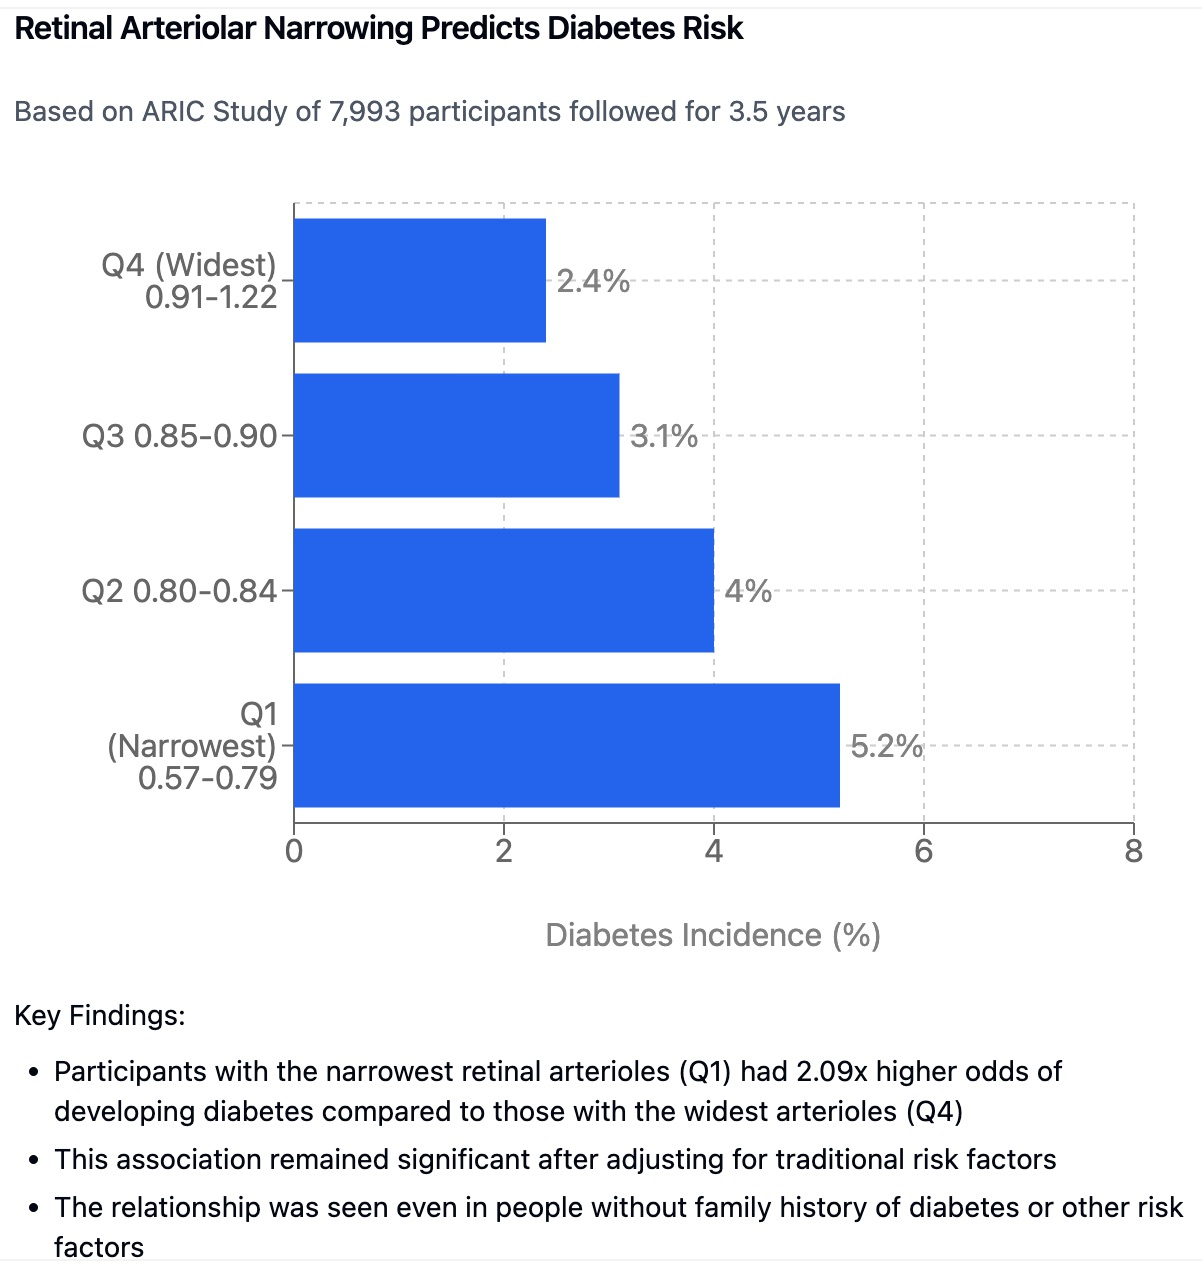
\includegraphics[keepaspectratio]{_resources/images/research/Fundus_Photography_for_Early_Diabetes_Detection_-_Claude.jpg}}

}

\caption{来源: Wong (2002)}

\end{figure}%

对于现代临床实践,这些发现突显了眼底摄影作为早期和整体健康评估的强大工具的潜力。在传统诊断测试显示异常之前揭示视网膜微血管早期变化的能力使及时干预和生活方式修改成为可能。其非侵入性使其对可能对传统医疗程序犹豫的患者特别易于接受和吸引人。该技术无缝集成到更广泛的健康和健康评估中,不仅提供有关眼部健康的见解,还提供有关系统性疾病的信息。作为监测工具,连续视网膜图像可以随时间追踪糖尿病的进展和治疗效果,实现更有针对性和有效的护理。

视网膜健康与糖尿病之间的联系现已确立,高分辨率眼底摄影代表了通过早期检测、增强监测和更全面的健康视角改善患者结果的显著机会。AI的整合使这项技术的获取民主化,使复杂分析可供广泛的从业者使用。这种方法在预防和健康护理中特别出色,为提供者和患者提供有价值的见解,同时使个人能够主动控制他们的健康之旅。

\section{其他眼部病理学}\label{ux5176ux4ed6ux773cux90e8ux75c5ux7406ux5b66}

青光眼,另一种与各种系统因素相关的常见眼部疾病,也可以通过应用于眼底照片的AI算法识别\footnote{Milea
  等 (2020)}。这些发现可能具有临床影响,因为青光眼是失明的常见原因,并可能早期筛查和治疗。除此之外,一些研究人员已经探索了甲状腺疾病与视网膜眼底图像之间的联系,并发现了有希望的诊断应用,尽管需要进一步工作。

高血压视网膜病变(HPR)在眼底图像中表现出AI系统现在可以可靠检测的独特模式。研究表明,HPR变化的严重程度与系统性血压水平之间存在强烈相关性。先进的图像分析可以量化与HPR相关的小动脉狭窄、动静脉交叉变化和其他特征变化,提供有关心血管健康风险的有价值信息。

视盘玻璃膜疣,虽然通常被视为良性发现,有时可能与更严重的情况如视盘水肿混淆。AI驱动的分析通过检查视盘外观的特定特征帮助区分这些情况。研究表明,机器学习算法在区分玻璃膜疣与其他视盘异常方面能够达到高精度,有助于指导适当的临床管理。

AI分析对年龄相关性黄斑变性(AMD)的检测已显著增强。深度学习系统现在可以识别AMD的早期迹象,包括微妙的玻璃膜疣形成和色素变化,在它们在临床上变得明显之前。这种早期检测能力对于实施预防措施和减缓疾病进展至关重要。

分支视网膜静脉阻塞(BRVO)和中央视网膜静脉阻塞(CRVO)在眼底图像中呈现AI系统现在可以高度可靠地识别的独特模式。最近的研究表明,深度学习算法能够早期检测这些情况,可能使更快干预和更好的结果成为可能。

图像分析的最新进展也改善了视网膜动脉阻塞的检测。AI系统现在可以识别血管口径和灌注模式的微妙变化,这可能表明即将发生阻塞事件。这种能力可以帮助识别这些威胁视力的情况风险的患者,在它们在临床上变得明显之前。

通过眼底成像检测视神经炎也从AI分析中受益。机器学习算法可以识别视盘外观和视乳头周围视网膜神经纤维层的微妙变化,这可能表明炎症或脱髓鞘过程。这种能力对于监测多发性硬化等疾病特别相关。

\section{视网膜成像与心血管健康}\label{ux89c6ux7f51ux819cux6210ux50cfux4e0eux5fc3ux8840ux7ba1ux5065ux5eb7}

人眼越来越显示为一面反映循环系统整体健康的复杂镜子。在视网膜内,一个精细的血管网络------小动脉和小静脉------提供了一个独特的、非侵入性的机会来观察系统性血管健康。这些微血管,通过非散瞳眼底摄影容易看到,会经历微妙但显著的变化,这些变化与发展缺血性心血管疾病(ICVD)风险增加相关。这些变化,包括但不限于小动脉直径变化、小静脉扩张和微血管损伤的存在,都表明身体更广泛血管系统的潜在功能障碍。在本节中,我们将探讨将视网膜微血管与ICVD联系起来的不断增长的证据。

评估心血管健康的传统方法,如血液检测、血压测量和问卷调查,提供了基本但有时不完整的风险图景。这些测试通常需要侵入性程序和/或复杂解释,并且可能难以在社区或初级保健环境中大规模部署。此外,CVD的风险评估仍然受到依赖传统风险因素的限制,因为许多没有这些风险因素的患者仍然发展心脏病。视网膜成像,特别是当与先进图像分析和人工智能(AI)结合时,为更直接和易于获取的人血管健康评估提供了一种新颖的、非侵入性途径,以及可以轻松部署在广泛临床和社区环境中的工具。研究的一个最引人注目的领域是开发能够从视网膜图像预测ICVD风险的AI驱动方法,这些方法在几个大型人口研究中显示了显著性能。

发表在《科学通报\footnote{Ma 等 (2022)}中的一项研究详细介绍了中国研究人员如何利用超过390,000张视网膜图像的庞大数据集训练深度学习算法进行ICVD风险分层。这项研究基于非散瞳眼底图像,使其易于在大多数临床环境中收集。该算法旨在通过学习识别眼底图像中可能对肉眼不明显的模式来估计患者10年内ICVD事件的风险,如微血管的微妙变化。该模型在内部和外部验证数据集中都表现异常好,展示了在不同人群中的稳健性和通用性。该模型在内部数据集上实现了令人印象深刻的调整R²为0.876,在外部验证集(北京衰老和血管研究(BRAVE)数据集)上为0.638。调整后的R2代表了这个模型可以解释的变异性比例。R2为1表示模型完美预测结果,没有方差,而0代表模型没有预测结果的能力。这些结果表明,AI驱动的视网膜成像评估具有高潜力估计ICVD风险。

此外,当使用训练过的算法分类ICVD风险时,该模型在检测10年ICVD风险≥5\%的患者方面显示了非常高的受试者操作特征曲线下面积(AUC)。在内部验证数据集中,AUC为0.971(95\%置信区间:0.967-0.975),在外部验证中为0.859(95\%置信区间:0.822-0.895)。对于更高的ICVD风险阈值(≥7.5\%),内部验证数据集的AUC为0.976(95\%置信区间:0.973-0.980),外部数据为0.876(95\%置信区间:0.816-0.937)。接近1的AUC值表示完美的诊断准确性。这些AUC值展示了该算法的高预测能力,这与其他研究也看到基于眼底图像的AI算法具有高预测能力一致。结果表明,该算法可能是评估ICVD风险的既定方法的可行且准确的替代方案,这可能导致视网膜成像在常规检查中的广泛实施。这些发现还表明,AI算法能够学习微血管变化与ICVD的关联,包括小静脉扩张和小动脉狭窄。AI可以从图像中提取微妙的关系,这些关系虽然难以用肉眼欣赏,但可以预测健康结果。这些微妙的变化也与其他传统风险因素一致,如血压。

研究作者指出了一些限制。首先,数据是横断面收集的,其结果是从使用传统风险因素的估计工具预测的,而不是实际的纵向ICVD事件数据。为了确认预测能力,计划对BRAVE数据进行跟踪研究。其次,数据集中缺少吸烟状态。尽管有这些限制,这些发现仍然提供了令人信服的证据,证明AI在使用视网膜图像进行ICVD风险评估方面的潜力,考虑到方法的简单性和高度的预测能力。

\section{大脑和认知健康}\label{ux5927ux8111ux548cux8ba4ux77e5ux5065ux5eb7}

视网膜在发育过程中是大脑的胚胎延伸,因此与大脑共享密切的生理和解剖关系\footnote{Cheung
  等 (2014)}。它是一种不寻常的组织,可以非侵入性地观察,允许轻松检查微血管功能。正是因为这一点,科学家们正在探索视网膜成像在理解脑血管和神经退行性疾病(如痴呆症)方面的潜在作用。视网膜图像提供了一种监测大脑健康的新方法。

越来越多的研究建立了视网膜血管变化与痴呆风险增加之间的相关性。研究表明,具有视网膜微血管异常(包括小动脉狭窄、小静脉扩张和视网膜病变的存在)的个体更可能发展认知下降和痴呆(Hua
等
2022)。这种联系植根于视网膜和脑微血管的相似性。两种血管系统共享类似的结构和生理功能,一种变化可能反映另一种中类似的病理变化。这种关系的含义很重要,因为脑血管疾病被认为是痴呆的主要贡献者。与单独依靠传统认知测试不同,视网膜成像可用于全人群筛查,识别高风险患者并允许更早干预。

在一项创新研\footnote{Kivipelto 等 (2006)}中,研究人员开发了一种利用眼底照片估计心血管风险因素、衰老和痴呆发病率(CAIDE)痴呆风险评分的新算法。CAIDE是一种成熟的工具,使用多维风险因素(年龄、性别、教育水平、身体不活动、收缩压、总胆固醇和体重指数)预测20年痴呆风险。研究表明,该算法与实际评分相比,预测CAIDE风险评分具有高调整R2(内部验证为0.80,外部验证为0.58),表明该算法能够从视网膜照片中提取相关数据。此外,该算法的外部验证显示具有高接收者操作特征曲线下面积(AUC)0.926(95\%置信区间:0.913-0.939),表明能够强力区分具有高痴呆风险的个体。这种预测能力非常令人印象深刻,因为CAIDE评分也已经在大型多种族人群中显示预测性。这项研究超越了简单相关,展示了AI驱动的视网膜图像分析可以预测与痴呆风险相关的复杂指标,表明非侵入性早期检测和风险分层的路径。

中国的一项类似研究\footnote{Hua 等 (2022)}使用了来自19个地区271,864名参与者的眼底照片,在20,690名参与者上进行外部验证。该算法使用相同的CAIDE风险评分识别高痴呆风险方面显示出显著准确性,在内部验证中达到AUC
0.944,在外部验证中达到0.926。

该算法在估计和实际CAIDE评分之间显示出强相关性,特别是在内部验证组(R²=
0.80)。重要的是,较高的估计风险评分与多个领域的认知表现较差显著相关,确认了预测的临床相关性。

重要的是指出,该研究是横断面而非纵向的,在外部验证中显示较低相关性(R²=
0.58),并且仅限于中国人群。此外,开发数据集缺乏可能改善预测的完整生活方式数据。

尽管有这些限制,这代表了在系统健康筛查中使用视网膜成像的重大进步。在不同人口统计群体和风险阈值之间的强表现表明,这项技术可以帮助识别早期干预和临床试验招募的风险个体,尽管进一步验证与纵向结果数据将是有价值的。

进一步支持视网膜和大脑之间这种联系的是检查环境因素对视网膜结构影响的工作。伦敦大学学院的研究人员分析了英国生物库数据集,确定暴露于环境空气污染可能与视网膜层厚度变化有关\footnote{Chua
  等 (2020)}。他们发现,增加暴露于细颗粒物质(PM2.5)和氮氧化物与视网膜神经纤维层(RNFL)增厚和神经节细胞-内丛状层(GCIPL)变薄相关。此外,更高水平的PM2.5吸收与RNFL、内核层和OPL+ONL变薄相关。这些发现不仅表明环境毒素对视网膜结构的影响,还暗示这些相同的毒素也可能在其他区域,包括大脑中引起类似变化。

总的来说,这些调查表明,基于AI的视网膜图像分析潜在可以提供早期、非侵入性的大脑健康指标,提供一个窗口了解可能先于神经退行性疾病如痴呆症的病理过程。

\section{视网膜成像与贫血}\label{ux89c6ux7f51ux819cux6210ux50cfux4e0eux8d2bux8840}

除了作为血管和神经健康的窗口之外,视网膜还提供了一个非侵入性评估贫血等血液学状况的独特机会。贫血,以红细胞或血红蛋白缺乏为特征,影响全球估计16亿个人,在诊断和管理方面面临重大挑战\{{[}\}1,2\{{]}\}。由于需要血液样本的诊断测试的侵入性和成本,这种情况常常未被诊断,特别是在资源有限的环境中。然而,AI的最新进展,特别是当应用于视网膜眼底照片时,为这种重要状况的非侵入性检测和管理提供了一个有希望的替代方案。

研究人员已经证明,AI算法可以仅使用眼底照片准确量化血红蛋白(Hb)水平并检测贫血的存在。在一项发表在《自然生物医学工程》\footnote{Mitani
  等 (2019)}的大规模研究中,一组科学家使用英国生物库的眼底图像开发了深度学习模型,使用眼底照片、参与者元数据或两者结合来检测贫血。他们发现,眼底图像与元数据的组合模型最为准确,研究使用了11,388名研究参与者的验证集。组合模型的结果显示,预测Hb浓度的平均绝对误差(MAE)为0.63
g/dL(95\%置信区间,0.62-0.64),贫血检测的AUC为0.88(95\%置信区间,0.86-0.89),任何贫血检测的ROC曲线下面积为0.88(95\%置信区间0.86-0.89),中度至重度贫血的ROC曲线下面积为0.95(95\%置信区间,0.93-0.97)。MAE
0.63 g/dl接近实验室测量的0.14
g/dl(参考)精度,比非侵入性即时护理设备的精度1.1至1.2
g/dl要高得多。这些结果令人震惊,因为这些结果完全基于非侵入性测量。眼底照片捕捉了与低血红蛋白相关的微妙变化,包括视网膜苍白和静脉迂曲度。这些发现不仅强调了深度学习在处理复杂图像数据方面的能力,还显示了非侵入性诊断贫血方法的明确路径。

此外,研究还发现,该算法可以在539名自报糖尿病的参与者中检测贫血,性能相当。研究的MAE略大,为0.73
g/dl(95\%置信区间,0.68-0.78
g/dl),AUC为0.89(95\%置信区间,0.85-0.93),相比于研究中的所有参与者。这些结果特别相关,因为贫血经常与糖尿病相关(高达23\%的糖尿病患者仍未被诊断出贫血)并且已经显示增加这些人群的发病率和死亡率。鉴于糖尿病视网膜病变的常规视网膜筛查的潜力,AI从视网膜照片中检测贫血的能力可能非常有用,并提供额外的健康筛查机会。

\section{瞳孔大小和智能}\label{ux77b3ux5b54ux5927ux5c0fux548cux667aux80fd}

基线瞳孔大小和认知能力之间存在一种有趣的相关性,进一步支持眼睛作为大脑功能窗口的作用。在佐治亚理工学院进行的研\footnote{Tsukahara
  和 Engle (2021)}表明,基线瞳孔较大的个体倾向于在流体智力、注意力控制和工作记忆容量测试中得分更高。这种关系足够稳健,以至于高低认知表现者之间的差异可以用肉眼检测到。

这种联系的生理基础在于蓝斑,这是上脑干中的一个核,调节瞳孔大小并在整个大脑释放去甲肾上腺素。这种神经递质在感知、注意力、学习和记忆中起着关键作用。更重要的是,它有助于维持跨远距离区域的有组织大脑活动------这一功能对复杂认知任务至关重要。

研究团队使用高精度眼动追踪技术,在受控照明条件下测量参与者执行各种认知评估时的瞳孔大小。瞳孔直径通常范围为二至八毫米,与流体智力测试和注意力控制任务的表现显示一致正相关。一项特别揭示性的测试要求参与者抵抗观看闪烁刺激,而是专注于识别短暂显示的字母------这是一项需要精密注意力控制的任务。

瞳孔大小和认知功能之间的这种联系似乎是年龄依赖性的,年长参与者通常显示更收缩的瞳孔。然而,当按年龄调整时,瞳孔大小和认知能力之间的关系仍然显著。这一发现表明通过精确瞳孔测量进行非侵入性认知评估的潜在应用。

一种假设认为,较大的基线瞳孔大小表明蓝斑的强化调节,可能反映更有效的大脑组织。这可能解释与更高认知表现的相关性。值得注意的是,蓝斑功能障碍已被牵连到阿尔茨海默病和ADHD等状况,表明仔细瞳孔测量在认知健康评估中的潜在诊断应用。

这项研究诠释了看似简单的生理测量如何提供复杂大脑功能的窗口。虽然需要更多研究来充分理解这些关系,但这些发现强化了全面眼部评估在健康评估中的价值。对于使用先进成像技术的从业者来说,意识到这些相关性可以增强他们对眼睛作为整体健康和认知功能生物标志物作用的理解。

\section{预测年龄和死亡风险}\label{ux9884ux6d4bux5e74ux9f84ux548cux6b7bux4ea1ux98ceux9669}

虽然传统智慧可能将视网膜仅与视觉功能联系起来,但研究越来越表明,眼睛还提供了观察衰老过程和量化死亡风险的窗口。视网膜,由神经组织和血管组成,反映了受年龄影响的局部变化以及衰老对人体更广泛的系统性影响。研究人员发现,通过眼底摄影可以识别视网膜与年龄相关的微妙变化,并使用AI进行量化,创建一个生物年龄和其与死亡风险联系的新型生物标志物。

新加坡的一组研究人员开发了一种算法,可以根据眼底图像的深度学习估计患者的生物年龄,称为RetiAG\footnote{Nusinovici
  等 (2022)}。该算法最初在40,480名韩国成人的眼底照片上训练,然后使用英国生物库的56,301名参与者进行评估,这证明了其在不同人群和种族之间的通用性。他们发现,使用年龄大于或等于65岁的截止点,该算法显示AUC为0.76,AUPRC为0.399。更重要的是,他们然后按RetiAGE对参与者进行分层,并追踪他们超过10年,发现RetiAGE第四四分位数的个体与最低四分位数相比,全因死亡风险增加67\%,CVD相关死亡风险增加142\%,癌症相关死亡风险增加60\%。关键的是,这些关联独立于年龄和一些既定的衰老生物标志物,包括白蛋白、肌酐、葡萄糖和C反应蛋白。这些数据表明,该算法捕捉了一些传统生物标志物无法识别的与衰老相关的生物变化。在这项研究中,研究人员还表明,RetiAGE的添加增加了预测死亡风险的能力,超越了传统风险因素。

\begin{figure}[H]

{\centering \pandocbounded{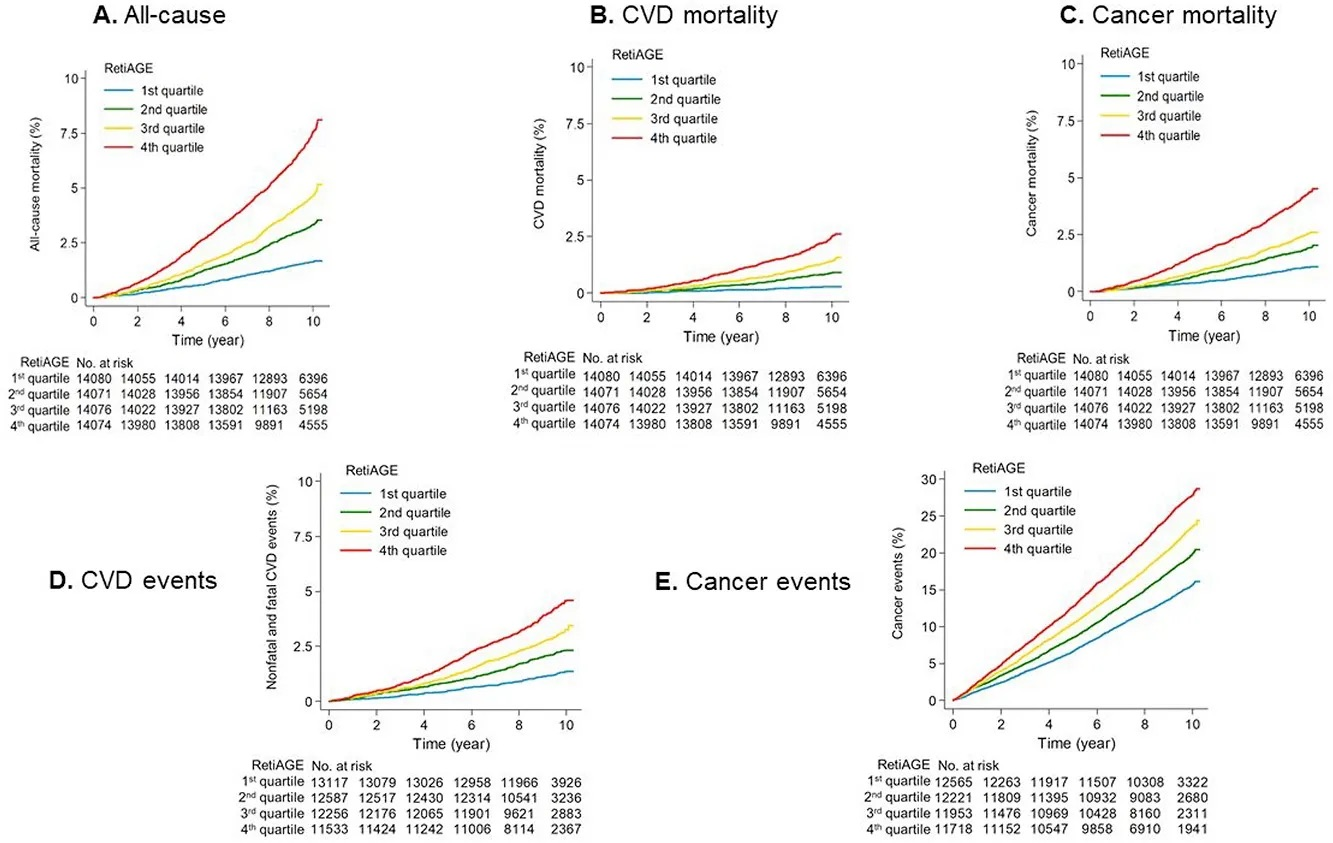
\includegraphics[keepaspectratio]{_resources/images/RetiAgeMortality-Nusinovici.jpg}}

}

\caption{视网膜年龄与许多其他死亡率指标良好对应。来源: Nusinovici et
al.~(2022a)}

\end{figure}%

类似地,另一项基于英国生物库眼底图像10年纵向分析的研究发现,视网膜年龄差距(预测年龄与实际年龄之间的差异)与全因死亡风险增加2\%和非CVD/非癌症死亡风险增加3\%相关\footnote{Zhu
  等 (2023)}。虽然他们没有发现视网膜年龄差距与CVD或癌症相关死亡率之间的显著关联,但他们的发现强调了视网膜变化在更广泛衰老过程中的作用。上述两项研究都具有强烈的统计显著性,有大型人群和严格的方法,从而支持视网膜眼底成像可能提供确定生物年龄和死亡风险的非侵入性方法的假设。

虽然与年龄和死亡率相关的观察到的视网膜变化背后的生物机制仍然是未来研究的主题,但越来越明显的是,AI驱动的视网膜图像分析可以提供生物衰老和长期健康结果的新型标记,展示作为在各种不同环境中评估死亡风险的工具的显著潜力。

\section{超越主要焦点}\label{ux8d85ux8d8aux4e3bux8981ux7126ux70b9}

支持使用眼底摄影进行一般健康评估的证据库继续增长\footnote{Lin 等 (2021)},超越心血管、神经和血液学状况。AI正在证明是一种多功能工具,其分析视网膜图像复杂性的能力正在扩大我们对视网膜及其与一系列系统性疾病联系的理解。

例如,研究表明通过视网膜分析评估肝功能的潜在应用。视网膜的独特血管模式可能反映与肝脏状况相关的微妙变化,因为两个器官共享类似的微血管特征和调节机制。早期研究表明,特定视网膜血管模式可能与肝酶水平和功能相关,尽管需要更多研究来验证这些发现。

新兴证据还指向免疫学评估的潜在应用。视网膜的免疫特权状态及其与系统免疫的复杂关系使其成为监测免疫系统功能的有趣目标。视网膜血管和组织特征的变化可能提供自身免疫状况或免疫系统功能障碍的早期指标。

激素平衡可能是视网膜成像可能提供见解的另一个领域。视网膜包含众多激素受体,初步研究表明激素波动可能影响视网膜血管特征。这可能为内分泌系统功能提供非侵入性窗口,尽管仍需进行大量验证工作。

研究人员还在探索视网膜模式与胃肠道健康之间的联系。肠-脑轴,越来越显示影响健康各个方面,可能在视网膜组织中表现出可观察到的变化。一些研究表明,炎症性肠病可能反映在视网膜血管模式中,尽管这些发现仍处于初步阶段。

视网膜成像评估线粒体功能的潜力代表了另一个令人兴奋的前沿。鉴于视网膜的高代谢需求和密集线粒体网络,视网膜组织特征的变化可能反映系统线粒体健康。这可能对理解能量代谢和与年龄相关的状况有影响。

随着分析能力的进步,研究人员正在调查视网膜特征与微生物组健康之间的潜在相关性。虽然这种联系乍看起来似乎不太可能,但新兴研究表明,肠道微生物组成可能通过系统炎症途径影响视网膜健康。

时间生物学领域也可能从先进视网膜分析中受益。视网膜在昼夜节律调节中的作用表明,详细成像可能提供关于昼夜节律扰乱及其系统性影响的见解。这可能对睡眠医学和代谢健康评估产生影响。

这些新兴研究领域强调了视网膜成像应用的持续演变。随着AI系统分析更大数据集并识别新模式,我们可能会发现视网膜特征与健康各个方面之间的其他相关性。然而,在探索这些新可能性时,保持科学严谨性很重要。

未来可能会揭示视网膜健康与系统性疾病之间更多意想不到的联系。随着我们对身体相互连接系统理解的加深,视网膜作为整体健康窗口的角色可能会扩大。这强调了在评估视网膜成像技术的新应用时,保持开放但批判性思维的重要性。

这一持续研究强化了将视网膜成像纳入全面健康评估的价值。虽然一些应用仍然是推测性的,但不断增长的证据表明,眼底摄影将继续揭示关于人类健康和疾病过程的新见解。

这些发展仅仅代表着先进视网膜成像可能实现的开端。随着技术继续演变和我们理解的加深,我们可以期待发现额外的应用,进一步增强这种非侵入性评估工具在健康实践中的价值。

\bookmarksetup{startatroot}

\chapter{现代视网膜成像技术}\label{ux73b0ux4ee3ux89c6ux7f51ux819cux6210ux50cfux6280ux672f}

\section{引言}\label{ux5f15ux8a00}

将先进的视网膜成像技术整合到健康实践中,代表了增强患者护理并构建更可持续商业模式的重要机会。本章探讨了现代眼底相机技术的基础,特别是关注近期技术进步如何促成了新的视网膜成像方法,这些方法优先考虑便携性、易用性和可负担性。

\section{眼底相机技术的演变}\label{ux773cux5e95ux76f8ux673aux6280ux672fux7684ux6f14ux53d8}

半个多世纪以来,眼底相机一直是眼科实践的专属领域,代表了每台设备超过5万美元的重大投资。这些早期设备重量在20-35千克之间,需要专用的检查室,具备精确的环境控制和特殊的电气要求。操作这些设备需要广泛的培训,因为即使是轻微的错位也可能损害图像质量。这些系统的复杂性意味着一次图像捕捉可能需要15-20分钟的仔细调整和患者定位。

传统眼底相机依赖复杂的闪光系统和基于胶片的摄影,需要仔细校准和维护。1990年代向数字传感器的过渡标志着重大进步,尽管早期的数字系统仍然保留了其基于胶片前辈的体积和复杂性。这些相机主要用于诊断眼疾,如糖尿病视网膜病变、青光眼和黄斑变性,其高成本因其在眼科治疗中的关键作用而显得合理。

眼底相机技术的转型始于2000年代初的几个并行发展。由手机行业推动的高分辨率CMOS传感器的出现,为以传统CCD系统成本的一小部分进行图像捕捉提供了新的可能性。LED技术的进步促成了更高效、紧凑的照明系统,可以取代早期设计中笨重的闪光管。同样,光学制造的改进,特别是在非球面元件的精密模塑方面,允许开发更小、更轻的光学系统,同时保持甚至提升传统设计的图像质量。

或许最重要的是,数字处理和人工智能的整合从根本上改变了视网膜成像的可能性。现代系统可以补偿轻微的错位,自动调整以适应患者差异,并为最佳图像捕捉提供实时指导。这些能力结合尺寸和成本的大幅降低,为将眼底摄影用于传统眼科环境之外开辟了新的可能性。

这些技术进步的汇聚促成了一代新型眼底相机,这些相机在保持专业级图像质量的同时显著减少了尺寸、复杂性和成本。这些现代系统重量低至2千克,几乎无需设置或培训,代表了视网膜成像技术的民主化,使其可供更广泛的医疗从业者使用。

\section{设计健康评估相机}\label{ux8bbeux8ba1ux5065ux5eb7ux8bc4ux4f30ux76f8ux673a}

将视网膜成像引入健康实践需要从基本原理重新思考传统眼底相机的设计。虽然眼科医生和眼科专家可以证明复杂、昂贵且需要专用操作员的设备是合理的,但健康从业者需要的是完全不同的东西------一个优先考虑可访问性、易用性和可负担性,同时保持专业级成像能力的系统。

或许最为关键的是,现代眼底相机必须在无需瞳孔扩大的情况下运行(非散瞳操作),因为药物扩瞳的要求将严重限制其在健康环境中的实用性。传统眼底摄影通常依赖散瞳滴剂来扩大瞳孔,为成像提供更方便的通道,但这带来了显著的实际障碍------患者需要等待20-30分钟让瞳孔扩大,随后会经历数小时的光敏感和视力模糊,且无法自己开车回家。这些副作用使得扩瞳在常规健康筛查中不切实际,并将严重限制患者的接受度。

\begin{tcolorbox}[enhanced jigsaw, coltitle=black, rightrule=.15mm, colback=white, colbacktitle=quarto-callout-note-color!10!white, breakable, bottomtitle=1mm, opacityback=0, bottomrule=.15mm, titlerule=0mm, opacitybacktitle=0.6, left=2mm, colframe=quarto-callout-note-color-frame, title=\textcolor{quarto-callout-note-color}{\faInfo}\hspace{0.5em}{为什么非散瞳操作至关重要?}, toptitle=1mm, toprule=.15mm, arc=.35mm, leftrule=.75mm]

瞳孔扩大(散瞳)传统上依赖于药物剂,如托吡卡胺、去氧肾上腺素或环戊托酸。这些药物通过刺激虹膜扩张肌(像去氧肾上腺素这样的α-肾上腺素能激动剂)或麻痹虹膜括约肌(像托吡卡胺这样的抗胆碱能药物)起作用。虽然这些药物能有效创建更大的成像窗口,但它们可能引发从暂时不适到严重医疗紧急情况的副作用。\newline{}

常见副作用包括光敏感、近视模糊和聚焦困难,可能持续4-6小时。在此期间,患者无法安全驾驶,并可能对其日常活动造成重大干扰。更令人担忧的是罕见但严重的反应,如急性闭角型青光眼,如果不及时治疗可能导致永久性视力丧失。全身效应可能包括心率加快、血压升高和中枢神经系统紊乱。\newline{}

对于某些医疗条件或服用特定药物的患者需要特别小心。例如,前房角狭窄的患者发生闭角型青光眼的风险较高。服用某些精神病药物的患者,特别是三环类抗抑郁药或单胺氧化酶抑制剂,可能经历危险的药物相互作用。\newline{}

因此,散瞳滴剂的管理需要:

\begin{itemize}
\tightlist
\item
  仔细筛选患者的禁忌症
\item
  适当的药物储存和处理
\item
  应对不良反应的紧急协议
\item
  眼科药物的专业培训
\item
  管理处方药的合法权限
\end{itemize}

这些要求使得散瞳成像不适合健康环境,在那里重点应放在安全、非侵入性评估上。非散瞳相机通过巧妙的光学和电子设计消除了这些风险和复杂性,同时保持成像能力。

\end{tcolorbox}

设计非散瞳操作在整个系统中引发了级联技术挑战。未扩大的瞳孔通常直径仅为2-4毫米,为照明和成像视网膜提供了更小的窗口。这一限制推动了对更复杂光学、更敏感成像传感器以及特别小心管理照明的需求。照明系统必须提供足够的照明以保证图像质量,同时保持患者舒适并避免触发瞳孔收缩从而进一步减少通道。

解决方案通常涉及多个子系统的仔细协调。红外LED提供不可见的照明用于初始对准和聚焦,因为即使通过小瞳孔,这些波长下的视网膜也能被清晰查看。当一切正确对准后,短暂的可见光脉冲会在瞳孔收缩前捕捉实际图像。整个序列必须自动且几乎瞬时发生,以确保未经培训的操作员也能获得一致的结果。

真正的便携性代表了另一个基本要求。与传统设置可能证明专用检查室合理不同,健康实践通常需要灵活性来决定如何以及在何处进行评估。这推动了对尺寸和重量的要求------整个系统必须足够轻(低于2.5千克)便于移动,且足够紧凑(任一维度低于300毫米)以适应标准桌子或桌面。这种便携性使实践能够最大化空间利用,甚至支持移动筛选服务。

自动化在为非专业操作员设计时变得至关重要。传统眼底相机需要患者定位、焦点调整和曝光控制方面的丰富专业知识。现代系统必须自动处理这些技术方面,使用高级瞳孔跟踪进行对准,自动聚焦系统和智能曝光控制。语音指导帮助操作员和患者完成成像过程,无需广泛培训。

光学系统必须平衡相互竞争的需求。虽然保持高图像质量仍然至关重要,但设计还必须适应不太理想的检查条件。视场角(通常为30-45度)必须为健康评估提供足够的视网膜覆盖,同时保持光学系统的紧凑性和可负担性。

互联网连接在考虑健康实践的需求时从可选变为必需。系统必须无缝集成云服务以进行图像存储、分析和报告生成。这种连接还支持自动软件更新和远程支持功能,这对于在无需现场技术专长的情况下维护系统性能至关重要。

成本管理影响设计的各个方面。虽然传统眼底相机可以证明整个系统中使用高端组件是合理的,但将这项技术引入健康实践需要对整个系统进行仔细优化。这意味着尽可能利用消费电子产品的进步(如手机行业的CMOS传感器),使用精密模塑而非研磨的光学组件,并在每个子系统中仔细平衡性能与成本。

其结果是对眼底相机设计的根本不同方法------一种优先考虑健康环境中实用性的方法,同时保持有意义的健康评估所需的基本能力。这种转变使视网膜成像可供全新类别的从业者使用,支持日益增长的更全面、技术支持的健康护理趋势。

\section{Opticare AI相机}\label{opticare-aiux76f8ux673a}

Opticare
AI眼底相机(型号AI-FD16aF)通过具体的工程实现体现了这些现代设计原则:

物理设计:

\begin{itemize}
\tightlist
\item
  尺寸:297 × 253 × 125毫米
\item
  重量:2千克
\item
  最小瞳孔直径:2.8毫米
\item
  视场角:40度
\end{itemize}

成像系统:

\begin{itemize}
\tightlist
\item
  1200万像素数字传感器,提供4000 × 3000像素分辨率
\item
  中心视场分辨率:≥ 60线对/毫米
\item
  中场分辨率:≥ 40线对/毫米
\item
  外围分辨率:≥ 25线对/毫米
\item
  屈光度调整范围:-15D至+15D(覆盖约95\%的人口)
\end{itemize}

照明:

\begin{itemize}
\tightlist
\item
  红外LED系统(770-930纳米)用于聚焦和对准
\item
  白光LED闪光(4500-6700K色温)用于图像捕捉
\item
  安全限制曝光时间(红外最大600秒,闪光20次曝光)
\item
  符合ISO 15004-2:2007眼科仪器安全性标准
\end{itemize}

连接性:

\begin{itemize}
\tightlist
\item
  USB 2.0/3.0接口用于数据传输和控制
\item
  HDMI输出用于外部显示
\item
  WiFi:双频(2.4/5 GHz),支持802.11b/g/n/ac
\item
  4G蜂窝支持
\item
  HTTPS安全数据传输
\item
  JPEG图像存储,具备云备份功能
\end{itemize}

操作参数:

\begin{itemize}
\tightlist
\item
  电源:100-240V交流,50/60 Hz,最大0.8A
\item
  温度范围:+5°C至+40°C(运行),-40°C至+55°C(存储)
\item
  湿度:10-90\%无冷凝
\item
  电磁兼容性:第1组B类设备
\item
  安全等级:II类电气,带B型患者保护
\end{itemize}

这些规格反映了为健康评估应用进行的仔细优化,在保持专业级成像能力的同时平衡了技术复杂性和实用性。

\bookmarksetup{startatroot}

\chapter{Opticare AI --
创新与健康的结合}\label{opticare-ai-ux521bux65b0ux4e0eux5065ux5eb7ux7684ux7ed3ux5408}

在当今快速发展的健康与保健领域,技术正在改变专业人士评估、监测和改善患者健康的方式。Opticare
AI眼底相机处于这一转变的前沿,这一创新工具将尖端成像技术与人工智能(AI)的力量相结合。本章探讨Opticare
AI如何弥合传统健康实践与最先进健康评估之间的差距,使从业者能够提升其服务水平,同时增强患者成果。

眼睛常被称为''心灵的窗户'',同时也是健康的窗口。通过分析视网膜,健康专业人士可以深入了解全身健康状况,提供无创、无痛的健康评估方法。对于寻求吸引精通技术、注重健康的客户的诊所来说,Opticare
AI相机是一个改变游戏规则的工具。

\section{Opticare AI --
健康报告与分析}\label{opticare-ai-ux5065ux5eb7ux62a5ux544aux4e0eux5206ux6790}

Opticare
AI系统通过全面的报告将复杂的视网膜数据转化为可行的健康洞察,解决健康的多个维度。本章详细探讨每项健康指标,解释其科学基础和对健康从业者的实际影响。

每份Opticare
AI报告都源自对高分辨率眼底图像的复杂分析,利用经过数百万标记视网膜图像训练的深度学习算法。报告在成像后几分钟内生成,并提供关于五个关键健康维度的见解:

\begin{enumerate}
\def\labelenumi{\arabic{enumi}.}
\tightlist
\item
  黄斑视力健康
\item
  循环系统健康
\item
  认知健康
\item
  代谢健康
\item
  心血管健康
\end{enumerate}

分析在图像捕获后立即开始,AI算法检查无数视网膜特征,包括血管模式、层结构和组织特征。这种多维分析允许进行全面的健康评估,远超传统的视力筛查。

\begin{figure}[H]

{\centering \pandocbounded{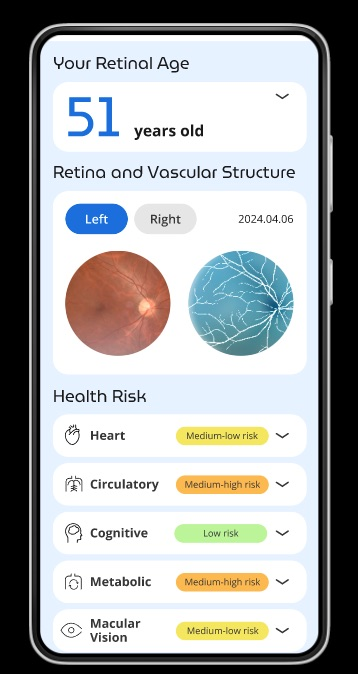
\includegraphics[keepaspectratio]{_resources/images/reports/OpticareSampleReport.jpg}}

}

\caption{Opticare AI报告样本}

\end{figure}%

\textbf{报告结构与呈现}

报告设计注重清晰度和可操作性,每个健康维度单独呈现。从业者可以选择将某些报告设为可选,只有在解锁后才能查看,从而允许灵活的服务模式和分阶段实施。这一功能对大规模筛查活动特别有价值,从业者可以免费提供一两份基本健康报告作为激励,同时为预约或支付小额费用解锁额外见解的客户保留全面结果。

Opticare报告的视觉设计通过直观的风险分类系统优先考虑直观理解。健康指标分为四个广泛类别,每个类别都有不同的颜色编码:

\begin{itemize}
\tightlist
\item
  低风险(绿色)
\item
  中低风险(黄色)
\item
  中高风险(橙色)
\item
  高风险(红色)
\end{itemize}

这种有意的简化服务于多种目的。首先,它承认基于AI的健康评估仍然是一门不断发展的科学,避免暗示可能误导人的精确度。其次,它以容易理解的格式呈现信息,客户可以快速理解。第三,它便于进行关于健康趋势的富有成效的对话,而不会因微小变化而造成不必要的焦虑。

每份报告包括:

\begin{itemize}
\tightlist
\item
  特定健康维度的总结分数
\item
  贡献因素的详细分析
\item
  比较数据,显示结果相对于同龄人群标准的位置
\item
  对回访客户的变化指标,突出改进或自上次评估以来的下降
\item
  进一步调查或干预的建议重点领域
\item
  可定制的建议,从业者可以根据其特定方法进行调整
\end{itemize}

报告可以广泛定制,以符合每个诊所的方法和品牌标识。从业者可以添加其徽标、联系信息,甚至预约功能,使客户轻松预约随访。建议部分特别灵活,允许从业者用反映其独特方法的具体指导取代通用建议------无论是营养策略、补充剂建议还是特定治疗方式。

这种结构化方法允许从业者快速掌握关键见解,同时可以在需要时获取更深入的信息。标准化格式还便于随时间比较,使有效监控对健康干预的反应变化成为可能。

\begin{tcolorbox}[enhanced jigsaw, coltitle=black, rightrule=.15mm, colback=white, colbacktitle=quarto-callout-caution-color!10!white, breakable, bottomtitle=1mm, opacityback=0, bottomrule=.15mm, titlerule=0mm, opacitybacktitle=0.6, left=2mm, colframe=quarto-callout-caution-color-frame, title=\textcolor{quarto-callout-caution-color}{\faFire}\hspace{0.5em}{警告:不用于诊断}, toptitle=1mm, toprule=.15mm, arc=.35mm, leftrule=.75mm]

我们必须反复强调:Opticare
AI系统目前未经FDA授权诊断或治疗任何疾病。以下讨论指出了使用先进的AI驱动眼底摄影理论上可能进行的诊断类型,\textbf{但当前的Opticare
AI系统不提供诊断}。任何与健康相关的结论必须由合格的专业人员做出至关重要。

\end{tcolorbox}

\section{视网膜年龄评估}\label{ux89c6ux7f51ux819cux5e74ux9f84ux8bc4ux4f30}

基于第2章讨论的研究,视网膜年龄评估提供了一个源自眼底成像分析的强大生物老化生物标志物。Opticare的复杂AI算法评估众多视网膜特征,确定''RetinalAge™``评分,这个评分通常与实际年龄不同,提供有关整体健康状况和寿命潜力的宝贵见解。

\textbf{分析的关键组成部分:}

\begin{itemize}
\tightlist
\item
  对视网膜微血管模式的详细评估
\item
  血管弯曲度和分支结构的评估
\item
  神经组织完整性和组织的分析
\item
  色素分布和组织密度的评估
\item
  与广泛规范数据库的比较
\end{itemize}

视网膜年龄评估的科学基础,如第2章所探讨的,来自显示视网膜特征与生物老化过程之间存在强相关性的里程碑研究。新加坡眼病流行病学研究和英国生物银行的研究表明,视网膜年龄差距(预测视网膜年龄与实际年龄之间的差异)是死亡风险和健康结果的重要预测指标。

当Opticare
AI系统生成RetinalAge™评分时,它不仅仅是估计眼睛看起来有多老,而是评估整个身体如何通过视网膜窗口反映出的老化情况。视网膜的独特属性------与脑组织共享的胚胎学起源、允许直接观察的透明性质以及丰富的微血管网络------使其成为评估整体生物老化的理想组织。

\textbf{理解报告:}

视网膜年龄评估提供几个关键指标:

\begin{itemize}
\tightlist
\item
  基于视网膜特征的估计生物年龄
\item
  与实际年龄的比较(视网膜年龄差距)
\item
  相比同龄人群的百分位排名
\item
  影响评分的具体贡献因素
\item
  对回访客户的趋势分析
\end{itemize}

RetinalAge™评分显著低于实际年龄表明健康的老化模式和潜在降低的年龄相关疾病风险。相反,超过实际年龄的视网膜年龄可能表明加速老化过程,需要进一步调查或生活方式修改。

\textbf{临床应用与现实期望:}

对于从业者来说,理解并传达视网膜结构随时间通常表现出显著稳定性很重要。与一些可能通过干预快速改善的生物标志物不同,视网膜变化往往是渐进和累积的。通过视网膜评估视角,健康干预的主要目标通常是减缓或阻止退化,而不是逆转现有变化。

从业者可以使用视网膜年龄评估来:

\begin{itemize}
\tightlist
\item
  建立监测未来变化的基线
\item
  确定预防措施可能最有益的领域
\item
  跟踪较长时间内的变化率
\item
  指导可能防止进一步退化的干预
\item
  为客户设定关于监测结果的现实期望
\end{itemize}

Opticare评估对于识别先前生活方式因素的影响特别有价值。例如,前吸烟者通常会显示反映过去暴露的永久视网膜变化。虽然这些变化可能不会逆转,但戒烟和其他积极干预可以显著减缓或阻止进一步退化------即使没有绝对分数的改善,这也是一项重要的健康成就,应该庆祝。

\begin{figure}[H]

{\centering \pandocbounded{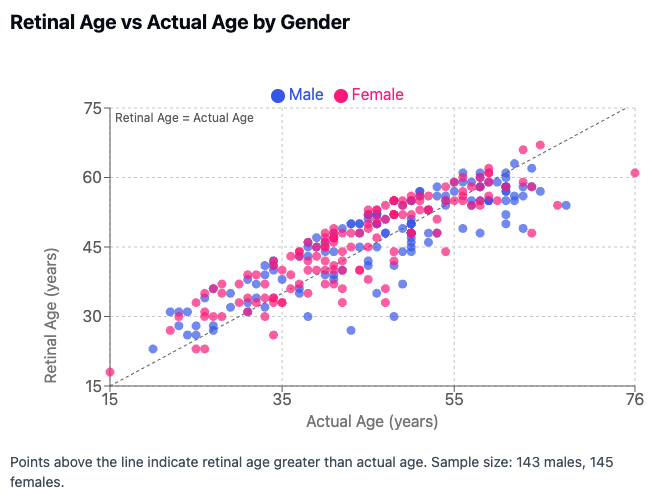
\includegraphics[keepaspectratio]{_resources/images/ch4/OpticareRetinalAge.png}}

}

\caption{RetinalAge™与实际年龄在Opticare用户样本中的相关性,数据点通常遵循线性趋势,但存在明显差异,表明年龄相似的个体之间的生物学年龄差异}

\end{figure}%

对于回访客户,随时间监测视网膜年龄稳定性提供关于健康干预有效性的客观反馈。成功通常不是通过分数改善定义的,而是通过维持稳定性(在原本预期会退化的情况下)定义的。这代表了一种更现实和科学合理的纵向监测方法。

视网膜年龄评估代表了AI驱动眼底摄影的最强大应用之一,提供了以前只能通过侵入性测试或复杂实验室分析获得的老化过程的见解。通过以可访问、非侵入性格式提供这种复杂指标,Opticare为健康从业者提供了一个有价值的工具,用于建立基线、识别风险因素并监测预防干预的有效性。

\section{黄斑视力健康}\label{ux9ec4ux6591ux89c6ux529bux5065ux5eb7}

基于第2章讨论的研究,黄斑视力健康评分评估对中央视力至关重要的视网膜结构。技术熟练的专业人士可以使用眼底图像来评估:

\begin{itemize}
\tightlist
\item
  黄斑完整性和潜在年龄相关变化的评估
\item
  视网膜神经纤维层厚度分析
\item
  玻璃膜疣存在和特征的评估
\item
  潜在血管异常的检测
\end{itemize}

该指标的科学基础来自将视网膜结构变化与眼部健康和全身条件联系起来的广泛研究。如第2章所讨论的,研究已经证明黄斑健康与各种全身条件之间存在强相关性,包括:

\begin{itemize}
\tightlist
\item
  年龄相关黄斑变性风险评估
\item
  糖尿病视网膜病变模式的早期检测
\item
  高血压视网膜病变迹象的识别
\end{itemize}

从业者可以使用这些信息来:

\begin{itemize}
\tightlist
\item
  指导预防性眼部护理建议
\item
  确定可能需要专科转诊的情况
\item
  监测当前健康干预的有效性
\end{itemize}

黄斑视力健康报告提供对中央视网膜的全面评估,突出优势和潜在关注领域。虽然避免具体诊断声明,但它提供了有价值的见解,可以指导健康建议并突出可能需要视力专家进一步调查的模式。

例如,报告可能表明黄斑结构的细微变化与年龄相关视力变化的已知风险因素相关。这些信息允许从业者讨论预防措施,如营养干预、蓝光保护或支持长期眼部健康的生活方式改变。

\section{循环健康}\label{ux5faaux73afux5065ux5eb7}

循环健康指标分析视网膜血管模式,提供关于全身血管健康的见解。这种评估包括:

\begin{itemize}
\tightlist
\item
  血管口径测量
\item
  动脉-静脉比率分析
\item
  血管弯曲度评估
\item
  微血管模式评估
\end{itemize}

借鉴第2章\footnote{特别是@ma\_deep\_2022}和随后研究中提出的研究,眼底图像可以反映:

\begin{itemize}
\tightlist
\item
  全身血管健康状态
\item
  潜在心血管风险因素
\item
  微循环功能
\end{itemize}

科学基础包括:

\begin{itemize}
\tightlist
\item
  视网膜血管特征与全身血压之间的相关性研究
\item
  将血管模式与心血管结果联系起来的研究
\item
  展示各种循环条件预测价值的研究
\end{itemize}

循环健康报告提供了对身体微血管系统的窗口,这常常反映更广泛的血管健康趋势。从业者可以使用这些信息来指导关于心血管健康策略的讨论,包括营养方法、运动建议和支持健康循环的压力管理技术。

对于回访客户,随时间跟踪血管模式的变化可以提供关于健康干预有效性的客观反馈。视网膜血管特征的改善通常与更广泛的血管健康改善平行,提供积极变化的有形证据,可以增强客户的动力和参与度。

\section{认知健康}\label{ux8ba4ux77e5ux5065ux5eb7}

认知健康评估利用将视网膜特征与神经系统健康联系起来的新兴研究。关键组成部分包括:

\begin{itemize}
\tightlist
\item
  视网膜神经纤维层分析
\item
  血管模式评估
\item
  结构完整性评估
\end{itemize}

基于第2章\footnote{参见@hua\_development\_2022关于CAIDE痴呆风险评分的工作}讨论的研究,该指标考虑:

\begin{itemize}
\tightlist
\item
  神经组织健康指标
\item
  与认知功能相关的血管模式
\item
  视网膜结构的年龄相关变化
\end{itemize}

科学基础包括:

\begin{itemize}
\tightlist
\item
  将视网膜变化与认知下降联系起来的研究
\item
  关于神经退行性疾病早期标记的研究
\item
  视网膜结构与脑健康之间的相关性研究
\end{itemize}

认知健康报告提供关于潜在神经健康模式的有价值见解,同时谨慎避免具体诊断声明。这些信息可以指导关于促进脑健康的生活方式实践的讨论,包括认知刺激活动、支持神经功能的营养方法和促进脑健康的体育活动。

对于专注于整体健康的诊所,认知健康报告提供了一个独特的机会,可以解决客户通常难以客观评估的健康方面。随时间可视化和跟踪神经健康标记的能力提供了一种有形的方式来讨论认知健康策略,这些策略可能看起来抽象或难以衡量。

\section{代谢健康}\label{ux4ee3ux8c22ux5065ux5eb7}

代谢健康评分源自将视网膜变化与代谢功能联系起来的广泛研究。这包括对以下内容的分析:

\begin{itemize}
\tightlist
\item
  微血管模式
\item
  血管壁特征
\item
  组织灌注指标
\end{itemize}

研究支持来自:

\begin{itemize}
\tightlist
\item
  关于糖尿病视网膜病变模式的研究
\item
  将代谢综合征与视网膜变化联系起来的研究
\item
  关于视网膜组织中胰岛素抵抗标记的调查
\end{itemize}

代谢健康报告提供与代谢功能相关的模式的见解,为这一关键健康方面提供独特的窗口。从业者可以使用这些信息来指导关于营养策略、体育活动建议和其他支持代谢健康的干预措施的讨论。

对于专注于体重管理、代谢优化或运动表现的诊所,这份报告提供了有关当前策略如何影响微血管水平代谢功能的有价值信息。当与可能没有看到传统指标(如体重或身体成分)即时变化但在代谢健康方面取得有意义进展的客户合作时,这一点特别有价值。

\section{心血管健康}\label{ux5fc3ux8840ux7ba1ux5065ux5eb7}

基于第2章\footnote{参见@ma\_deep\_2022关于ICVD风险的研究}中提出的研究,该指标评估:

\begin{itemize}
\tightlist
\item
  动脉特征
\item
  静脉模式
\item
  整体血管健康指标
\end{itemize}

科学基础包括:

\begin{itemize}
\tightlist
\item
  将视网膜模式与心血管结果联系起来的大规模研究
\item
  关于血管特征预测价值的研究
\item
  长期结果研究
\end{itemize}

心血管健康报告提供与心脏健康相关的模式的全面评估,补充传统心血管风险评估。这些信息可以指导关于心脏健康营养、适当体育活动、压力管理和其他支持心血管健康的干预措施的讨论。

对于已经纳入其他心血管评估的诊所,Opticare报告提供了互补信息,这些信息通常反映比传统测量(如血压或胆固醇筛查)可能检测到的更早期的变化。这种早期预警能力完美契合健康实践的预防重点。

\begin{figure}[H]

{\centering \pandocbounded{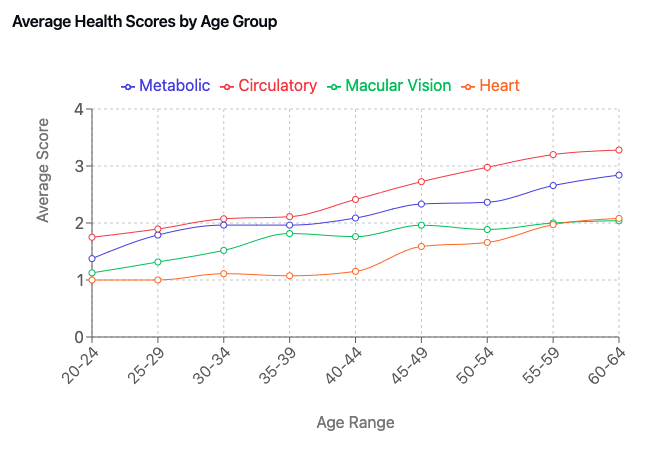
\includegraphics[keepaspectratio]{_resources/images/ch4/OpticareHealthScores.png}}

}

\caption{分数随时间增加(恶化)。数据来自最近数百名独特用户。由于这些是\_平均值\_,临床医生应更仔细观察与众不同的患者。}

\end{figure}%

\section{实际实施}\label{ux5b9eux9645ux5b9eux65bd}

\textbf{解读报告}

从业者应将这些报告视为对话的开始,补充其他临床发现,而非明确的诊断工具。这一观点与Opticare的理念(在第6章进一步探讨)一致,即使科学继续发展,现在提供先进技术比等待完美验证提供更大好处。

解读报告时的关键考虑因素包括:

\begin{itemize}
\tightlist
\item
  理解正常变异
\item
  识别显著变化
\item
  确定需要进一步调查的模式
\item
  将结果放在客户年龄范围的背景中解读
\item
  当出现矛盾时优先考虑已确立的临床发现
\end{itemize}

解读Opticare报告时,考虑绝对值和随时间的趋势都是至关重要的。单次测量提供有价值的基线信息,但最有意义的见解通常来自跟踪多次评估的变化。特定指标的改善或下降可以帮助评估健康干预的有效性并指导调整治疗计划。

年龄考虑在解读结果时特别重要。健康问题的患病率随年龄自然增加,因此风险指标往往在整个生命周期中遵循可预测的模式。二十几岁的年轻客户通常在各类别中主要显示''绿色''(低风险)结果,而六十几岁的客户可能通常显示更多''橙色''(中高风险)指标,而不一定有急性健康问题。在讨论结果时应考虑这种与年龄相关的进展。

当Opticare结果与其他临床发现矛盾时,从业者应优先考虑已确立的护理标准。例如,如果客户的HbA1c表明代谢问题,但其Opticare代谢健康报告显示低风险,从业者应遵循处理升高HbA1c的标准协议。相反,如果Opticare报告表明具有正常胆固醇和血压的客户有中高心血管风险,从业者应将其视为一个可能需要监测而非立即干预的单一数据点。技术应增强而非取代临床判断。

解读结果时,上下文至关重要。客户的年龄、整体健康状况、药物使用和最近的生活方式变化等因素都可能影响视网膜模式。Opticare
AI系统考虑了许多这些因素,但专业判断对于正确解读仍然至关重要。

虽然系统识别与各种健康维度相关的模式,但从业者在讨论结果时应保持适当的专业界限。重点应保持在健康促进和潜在问题的早期识别上,而非特定疾病诊断。将报告视为健康对话的开始,而非关于客户状况的最终结论。

\textbf{客户沟通}

关于报告发现的有效沟通包括:

\begin{itemize}
\tightlist
\item
  清晰解释指标
\item
  在整体健康评估中的背景
\item
  适当地构建结果
\item
  与其他临床发现的整合
\end{itemize}

与客户讨论Opticare报告时,视觉辅助可以显著增强理解。报告本身设计有清晰的图形,帮助客户快速掌握复杂信息。引导客户浏览每个指标,同时用日常术语解释其重要性,有助于建立理解和信任。

将讨论构建为健康优化而非疾病预测。例如,与其关注与某些模式相关的潜在负面结果,不如强调客户可以采取的积极步骤来支持报告涵盖的每个维度的健康。

将Opticare发现与健康评估的其他方面联系起来,创建关于客户当前健康状况和改进机会的连贯叙述。这种整合方法帮助客户看到全面评估的价值,理解各种健康方面如何相互关联。

使用报告作为协作目标设定的基础。指标的视觉性质使建立基线测量和设定特定、可衡量的改进目标变得容易。这种协作方法增强了客户参与和对其健康旅程的所有权。

\textbf{随访协议}

建立明确的协议:

\begin{itemize}
\tightlist
\item
  定期监测间隔
\item
  显著发现响应
\item
  转诊标准
\item
  进展跟踪
\end{itemize}

根据初始发现制定标准化随访时间表。例如,指标在最佳范围内的客户可能从年度重新评估中受益,而显示潜在关注模式的客户可能需要更频繁的监测,如季度或半年度随访。

创建明确的指导方针,说明何时的发现需要转诊给其他医疗提供者。在保持适当实践范围的同时,建立与能够提供更详细评估的专家的关系。记录您的转诊协议,确保所有客户获得一致、适当的护理。

实施系统性进展跟踪,允许轻松可视化随时间的变化。这可能包括跨多次评估的关键指标的图形表示,突出改进和需要持续关注的领域。

使用随访预约强化积极变化并解决挑战。回顾先前建议,评估遵从性,并根据主观反馈和视网膜模式的客观变化调整健康计划。

\section{与实践理念的整合}\label{ux4e0eux5b9eux8df5ux7406ux5ff5ux7684ux6574ux5408}

Opticare
AI系统与技术通常比传统科学验证过程更快的理念一致------这一概念在第6章中有更详细的探讨。这种前瞻性方法认识到,等待完全科学共识再采用潜在有益技术可能会延迟宝贵的护理机会。

将Opticare报告整合到您的实践理念中时,将其视为提供独特见解的创新工具,而非明确的诊断工具。它们的最大价值通常在于其能力:

\begin{enumerate}
\def\labelenumi{\arabic{enumi}.}
\tightlist
\item
  启动与客户的有意义健康对话
\item
  提供否则抽象健康概念的视觉表示
\item
  跟踪可能无法通过传统评估捕获的细微变化
\item
  在临床症状出现前提供潜在问题的早期指示
\item
  通过技术先进且可访问的评估增强客户参与
\end{enumerate}

这种方法既承认基于AI的眼底相机健康评估的潜力和局限性,又在全面健康实践中最大化其价值。通过将技术定位为多方面评估策略的一个组成部分,从业者可以利用其能力,同时保持适当的专业视角。

\section{结论}\label{ux7ed3ux8bba}

Opticare
AI健康报告提供了一种复杂而又易于理解的方式,利用视网膜成像进行全面健康评估。通过理解这些指标的科学基础和实际应用,从业者可以有效地将这项技术整合到他们的健康实践中,同时保持适当的专业界限。

将报告视为''对话的开始,而非结束''捕捉了其正确实施的精髓。这一观点认识到基于AI的眼底相机健康评估继续发展,即使科学继续发展,从业者和客户都从访问尖端技术中受益。

下一章将探讨Opticare系统在各种临床环境中的实际应用,基于对健康指标及其重要性的理解。

Opticare
AI报告源自设备的高分辨率眼底成像能力与深度学习算法的结合。报告在成像过程后快速生成,并总结患者在循环、认知、代谢和心血管健康等领域的潜在健康风险,以及特定眼部相关健康标记。该技术对易用性、速度和全面指标的关注确保这些报告对健康和保健专业人士既具可行性又易于理解。

\begin{figure}[H]

{\centering \pandocbounded{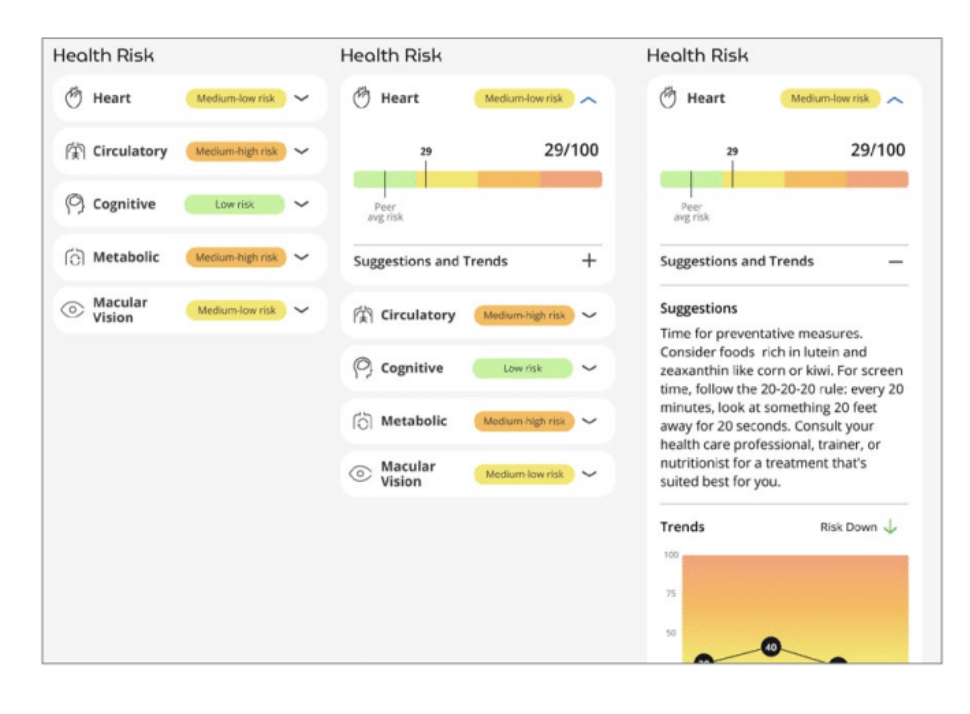
\includegraphics[keepaspectratio]{_resources/images/reports/ReportOther.png}}

}

\caption{健康评估功能}

\end{figure}%%
\begin{figure}[H]

{\centering \pandocbounded{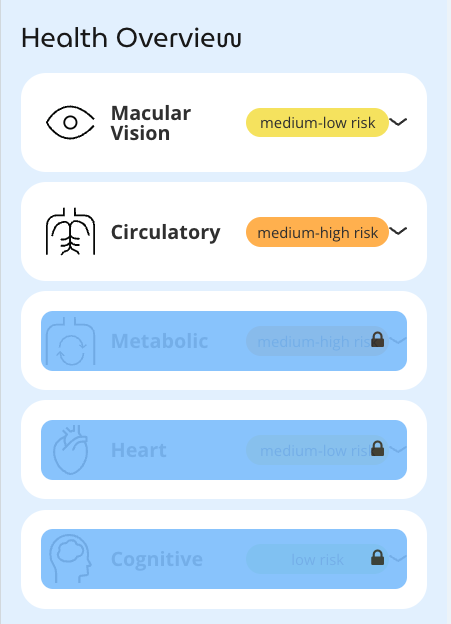
\includegraphics[keepaspectratio]{_resources/images/reports/ReportLocked.png}}

}

\caption{提供者可以选择让某些报告成为可选的,只有在解锁后才能查看。例如,在社区筛查环境中,潜在患者可能需要预约诊所预约才能解锁完整报告。}

\end{figure}%

\bookmarksetup{startatroot}

\chapter{在健康实践中的实际应用}\label{ux5728ux5065ux5eb7ux5b9eux8df5ux4e2dux7684ux5b9eux9645ux5e94ux7528}

将先进的视网膜成像技术整合到健康实践中代表着提升患者护理并建立更可持续商业模式的重要机会。本章探讨了将Opticare
AI相机整合到各种健康环境中的实用策略,并附有真实案例和实施指南。

\section{为成功做好准备}\label{ux4e3aux6210ux529fux505aux597dux51c6ux5907}

成功的准备始于对物理空间的周全考虑。Opticare
AI相机紧凑的设计和轻量化结构使其能够适应各种临床环境。仅有297mm × 253mm
×
125mm的尺寸和2kg的重量,该设备只需要最小的专用空间------通常一个约4x6英尺的适度检查区域就足够了。相机可以放置在小桌子或推车上,只需要基本设施:标准电源插座和可靠的互联网连接以传输结果。虽然空间不必过于精致,但应注意照明控制以确保最佳图像捕捉条件。舒适的患者座椅和基本的计算机设置完成了基本的物理要求。

员工培训是实施中的另一个关键考虑因素,尽管系统的直观设计大大减轻了这一负担。大多数实践发现,团队成员通过一天的实践经验就能掌握基本操作技能。培训过程自然从基本设备设置和维护进展到更细微的患者互动方面。员工学习正确的患者定位技术以确保一致、高质量的图像,以及常见技术问题的基本故障排除程序。也许最重要的是,他们发展与患者沟通成像过程并在适当的专业范围内解释结果的能力。

这种设置和培训过程的效率反映了Opticare对创造增强而非干扰现有健康实践的技术的承诺。无论是整合到脊椎按摩诊所、营养诊所,还是整体健康中心,该系统都能适应支持而非加重运营工作流程。

\section{实施}\label{ux5b9eux65bd}

实施始于明确的患者参与策略。Opticare成像过程是关于整体健康的优秀对话起点,特别是对于寻求扩展预防性护理服务的从业者。视网膜成像的非侵入性特性通常吸引那些可能对更传统的医疗筛查犹豫不决的人群,创造了有意义的健康讨论机会。向现有患者介绍这项技术时,成功的从业者强调其在全面健康监测中的作用。该过程自然与常规访问相配合,提供额外的数据点来跟踪整体健康模式随时间的变化。对于新患者获取,先进视网膜成像的可用性可以在日益竞争的健康市场中使实践脱颖而出。

移动筛查能力代表另一条有价值的实施途径。相机的便携设计使从业者能够在健康博览会、社区活动或企业健康计划中进行筛查。这些外展机会不仅服务于公共健康利益,还有助于建立实践知名度和客户基础。典型的移动设置只需要最少的设备:相机本身、笔记本电脑和基本筛查用品。许多从业者报告在当地农贸市场或社区中心设立''迷你诊所''取得了成功,快速、非侵入性的筛查过程吸引了注重健康的个人。

数据管理和整合是成功实施的关键组成部分。Opticare系统基于云的基础设施允许安全存储和轻松访问患者图像和报告。这个数字框架与大多数实践管理系统无缝集成,尽管从业者应建立明确的协议,将视网膜成像数据整合到现有的患者记录和健康计划中。

定价策略在实施过程中需要深思熟虑。虽然一些实践将视网膜成像作为标准健康评估的一部分,但其他实践则将其作为高级服务提供。关键在于有效地传达价值主张------帮助患者理解这种先进技术如何促进他们的整体健康旅程。从业者在制定定价模型时应考虑当地市场、患者人口统计和实践定位。

实施过程还受益于建立明确的结果沟通协议。虽然Opticare系统提供详细的健康见解,但从业者必须在其实践范围和专业边界内谨慎地构建这些发现。这通常涉及开发讨论结果的标准化语言和在发现建议需要额外医疗评估时的明确转诊途径。

\section{整合模式}\label{ux6574ux5408ux6a21ux5f0f}

\textbf{模式1:全面健康评估}

在此模式中,视网膜成像成为新患者标准初始评估的一部分。典型诊所:

``我们将Opticare
AI扫描作为所有新客户初始健康评估的一部分。它提供了有价值的见解,帮助指导我们的营养建议,并允许我们随时间跟踪变化。客户感谢这种技术化的健康监测方法。''

实施步骤:

\begin{enumerate}
\def\labelenumi{\arabic{enumi}.}
\tightlist
\item
  在初始咨询期间安排15分钟用于成像
\item
  将结果作为整体健康评估的一部分进行审查
\item
  利用见解制定个性化健康计划
\item
  安排适当间隔的后续扫描
\end{enumerate}

\textbf{模式2:移动健康筛查}

Opticare
AI相机的便携性使其成为移动筛查服务的理想选择。许多诊所在当地健康博览会和企业健康活动中取得了成功。这是向潜在患者介绍您的实践并提供有价值的健康见解的绝佳方式。扫描快速、非侵入性的特点使其非常适合这些环境。

移动筛查成功因素:

\begin{itemize}
\tightlist
\item
  适当的运输保护
\item
  可靠的移动互联网连接
\item
  清晰的教育材料
\item
  高效的录入流程
\item
  专业的设置展示
\item
  后续预约安排系统
\end{itemize}

\section{案例研究}\label{ux6848ux4f8bux7814ux7a76}

\begin{tcolorbox}[enhanced jigsaw, coltitle=black, rightrule=.15mm, colback=white, colbacktitle=quarto-callout-note-color!10!white, breakable, bottomtitle=1mm, opacityback=0, bottomrule=.15mm, titlerule=0mm, opacitybacktitle=0.6, left=2mm, colframe=quarto-callout-note-color-frame, title=\textcolor{quarto-callout-note-color}{\faInfo}\hspace{0.5em}{案例研究1:综合健康中心}, toptitle=1mm, toprule=.15mm, arc=.35mm, leftrule=.75mm]

典型健康中心的方法专注于将视网膜成像与其他健康评估相结合,提供全面护理。

实施策略:

\begin{itemize}
\tightlist
\item
  作为新患者工作的一部分提供成像
\item
  创建将成像与其他服务结合的套餐
\item
  建立季度跟踪协议
\item
  开发解释技术的教育材料
\end{itemize}

结果(前6个月):

\begin{itemize}
\tightlist
\item
  新患者保留率显著增加
\item
  平均患者参与时间增加
\item
  大多数现有患者选择了成像服务
\item
  对技术进步的积极反馈
\end{itemize}

\end{tcolorbox}

\begin{tcolorbox}[enhanced jigsaw, coltitle=black, rightrule=.15mm, colback=white, colbacktitle=quarto-callout-note-color!10!white, breakable, bottomtitle=1mm, opacityback=0, bottomrule=.15mm, titlerule=0mm, opacitybacktitle=0.6, left=2mm, colframe=quarto-callout-note-color-frame, title=\textcolor{quarto-callout-note-color}{\faInfo}\hspace{0.5em}{案例研究2:企业健康计划}, toptitle=1mm, toprule=.15mm, arc=.35mm, leftrule=.75mm]

这个团队将Opticare AI相机整合到他们的企业健康计划中,服务于多个企业:

实施策略:

\begin{itemize}
\tightlist
\item
  在合作公司定期举办健康日
\item
  个人筛查预约
\item
  与现有健康指标整合
\item
  定期进展报告
\end{itemize}

这个实践通过以下方式衡量其成功推出:

\begin{itemize}
\tightlist
\item
  服务的企业客户数量
\item
  筛查员工数量
\item
  后续计划的高参与率
\item
  增强的感知价值健康计划
\end{itemize}

\end{tcolorbox}

\section{收入模式和定价策略}\label{ux6536ux5165ux6a21ux5f0fux548cux5b9aux4ef7ux7b56ux7565}

\textbf{直接支付模式}

许多实践采用直接的服务费用模式取得成功:

\begin{itemize}
\tightlist
\item
  初次扫描:\$30-125
\item
  后续扫描:\$50-75
\item
  包含多次扫描的健康套餐:\$250-400
\end{itemize}

\textbf{会员模式}

一些实践将成像整合到健康会员计划中:

\begin{itemize}
\tightlist
\item
  月度会员:\$150-200
\item
  包含季度成像
\item
  绑定其他健康服务
\item
  优先预约安排
\end{itemize}

\textbf{企业计划定价}

对于服务企业的实践:

\begin{itemize}
\tightlist
\item
  每位员工筛查:\$45-65
\item
  企业健康套餐:\$2,000-5,000/月
\item
  大型组织的批量折扣
\item
  持续监测计划
\end{itemize}

\section{营销和患者教育}\label{ux8425ux9500ux548cux60a3ux8005ux6559ux80b2}

\subsection*{教育材料}\label{ux6559ux80b2ux6750ux6599}
\addcontentsline{toc}{subsection}{教育材料}

有效的患者教育是成功整合视网膜成像的关键基础。从业者应开发清晰、易懂的材料,解释技术及其在健康评估中的作用。这些教育资源通常包括说明成像过程及其益处的信息手册,以及帮助患者了解检查过程的视频演示。定期的通讯文章和社交媒体更新可以突出视网膜成像的价值,同时保持适当的专业界限,精心选择的案例研究可以说明该技术如何支持全面的健康护理。关键在于呈现赋予患者做出明智健康决定的信息,同时避免过于技术性的语言或营销炒作。

\textbf{营销渠道}

成功的视网膜成像服务营销需要保持专业诚信的多渠道方法。当地健康活动提供展示技术并与注重健康的社区成员联系的机会。专业网络建立与互补从业者的转诊关系,而现有患者通常通过结构良好的转诊计划成为倡导者。社区教育课程允许从业者分享关于眼睛健康和整体健康的知识,将自己定位为值得信赖的资源。社交媒体可以通过分享教育内容和实践更新来支持这些努力,尽管从业者应在网络存在中保持适当的专业界限。

\section{患者沟通策略}\label{ux60a3ux8005ux6c9fux901aux7b56ux7565}

\textbf{初始介绍}

向患者介绍视网膜成像服务时,从业者应强调其非侵入性方法和快速结果交付------通常在几分钟内可用。讨论应将视网膜健康模式与整体健康联系起来,同时强调早期检测的预防性益处。从业者可以解释成像过程如何与其现有的护理协议无缝整合,增强而非干扰已建立的治疗关系。这种解释应基于健康促进而非医疗诊断,帮助患者理解技术在其更广泛健康旅程中的作用。

\begin{tcolorbox}[enhanced jigsaw, coltitle=black, rightrule=.15mm, colback=white, colbacktitle=quarto-callout-note-color!10!white, breakable, bottomtitle=1mm, opacityback=0, bottomrule=.15mm, titlerule=0mm, opacitybacktitle=0.6, left=2mm, colframe=quarto-callout-note-color-frame, title=\textcolor{quarto-callout-note-color}{\faInfo}\hspace{0.5em}{示例介绍脚本}, toptitle=1mm, toprule=.15mm, arc=.35mm, leftrule=.75mm]

``作为我们致力于提供全面健康护理的一部分,我们使用先进的视网膜成像技术收集有关您整体健康状况的重要信息。这种快速、非侵入性的扫描只需几分钟,可以提供有价值的见解,帮助指导您的健康旅程。''

\end{tcolorbox}

\textbf{结果讨论}

与患者审查结果时:

\begin{itemize}
\tightlist
\item
  关注一般健康指标
\item
  避免特定疾病声明
\item
  强调生活方式联系
\item
  讨论预防策略
\item
  安排适当的后续
\end{itemize}

\textbf{开始使用}

成功整合视网膜成像的路径始于简单地开始使用。Opticare
AI系统的直观设计使通过实际经验学习成为最有效的方法。相机的便携性鼓励在传统临床环境之外创造性地实施------带到农贸市场、社区中心、教堂或企业健康活动。这种移动性使从业者能够在人们所在的地方与他们会面,消除参与障碍。

成功的从业者将视网膜成像用作患者保留和获取工具。许多人提供扫描作为非活跃患者回归的激励措施,通过提供尖端技术重新点燃这些有价值的关系。对于常规患者,添加视网膜成像表明致力于提供创新、先进的护理,不断增强他们的健康旅程。

价格灵活性允许各种战略方法。一些从业者提供特价''起步''扫描以鼓励初始参与,而其他人则将成像与现有健康套餐捆绑以提高感知价值。Opticare''随意使用''定价选项使实践能够在无使用限制的情况下扫描患者,支持高容量筛查活动或全面护理模式。

目标不是完美而是进步------开始使用技术,收集反馈,并根据实际经验完善您的方法。随着从业者对技术更加熟悉并更擅长沟通其益处,患者参与自然增加。通过优先行动而非过度规划,从业者可以更快地实现视网膜成像为其实践带来的价值。

\section{克服实施挑战}\label{ux514bux670dux5b9eux65bdux6311ux6218}

技术实施带来可管理的挑战,有远见的从业者预见并主动解决。互联网连接问题偶尔出现,特别是在移动筛查环境或高峰使用期间。成功的从业者维持备用连接选项,如移动热点,并建立定期IT系统检查,在问题影响运营前识别潜在问题。记录故障排除程序帮助员工快速、一致地解决常见问题。

图像质量优化需要注意环境因素和适当的患者定位。定期员工培训确保每个人理解遵循既定协议以获得最佳结果的重要性。许多实践开发简单的环境检查表,在每次成像会话前验证适当的照明和定位。这种系统方法有助于保持一致的质量,同时最小化重复捕捉的需求。

患者犹豫有时会形成初始障碍,尽管这通常通过清晰的教育和演示解决。透明的定价、技术益处的直接解释以及对过程非侵入性的保证通常能有效解决这些顾虑。患者见证和前后演示会话帮助潜在患者理解价值主张。后续遵从度通过自动提醒系统、清晰的价值沟通和使定期监测在经济上具有吸引力的健康套餐激励措施而提高。

\section{风险管理策略}\label{ux98ceux9669ux7ba1ux7406ux7b56ux7565}

实施创新技术不可避免地涉及管理新类型的风险。系统性的风险管理方法有助于保护从业者和客户。

详细的记录保存为风险管理提供基础。除了临床文档外,维护以下记录:

\begin{itemize}
\tightlist
\item
  技术性能指标和维护
\item
  员工培训和能力评估
\item
  客户沟通和同意讨论
\item
  协议遵从和任何偏差
\item
  技术问题和解决步骤
\item
  质量控制措施和结果
\end{itemize}

在实施新技术时,沟通日志需要特别注意。记录所有关于技术使用的重要讨论,包括:

\begin{itemize}
\tightlist
\item
  初始客户咨询和同意过程
\item
  对发现和局限性的解释
\item
  与其他提供者的转诊讨论
\item
  技术支持互动
\item
  客户问题和顾虑
\item
  跟进沟通
\end{itemize}

专业发展在风险管理中起着关键作用。定期培训确保所有员工保持对技术的能力。技术教育帮助从业者理解系统能力和限制。同行协作提供分享经验和最佳实践的机会。行业监测有助于识别新出现的问题和解决方案。

成功实施尖端技术最终取决于平衡创新与责任。通过理解证据基础、设定适当期望、维持专业标准和有效管理风险,从业者可以成功整合先进技术,同时为客户提供最佳护理。

\section{衡量成功}\label{ux8861ux91cfux6210ux529f}

视网膜成像整合的成功指标完全取决于您的实践目标。如果您的主要目标是实践增长,跟踪新患者获取、保留率和收入生成提供相关反馈。对于专注于临床结果的实践,监测干预效果、患者对建议的遵从度和健康标记改善可能更有意义。注重技术的实践可能优先考虑效率指标,如执行的扫描数量、与其他评估工具的整合和技术采用率。

质量保证代表另一个重要的成功领域。这包括定期设备维护、员工绩效评估和患者反馈收集。一致的协议遵从检查和准确性监测确保技术提供可靠、有意义的信息用于临床决策。许多实践建立这些指标的简单、定期审计,以维持高标准同时识别持续改进的机会。

最成功的实践保持其成功定义的灵活性,随着整合策略的演变调整指标。初始焦点可能集中在运营指标上,如成功的图像捕捉率,随着技术在实践中的确立,逐渐转向结果指标。这种适应性方法确保成功测量与当前实践优先事项和目标保持一致。

\section{未来增长机会}\label{ux672aux6765ux589eux957fux673aux4f1a}

视网膜成像服务的增长机会超出传统办公环境。移动筛查服务允许从业者将技术直接带给患者,而企业健康计划提供接触注重健康的员工群体的机会。社区健康活动和教育研讨会有助于建立意识和确立从业者专业知识。许多成功的实践将视网膜成像整合到全面的健康套餐中,创造增值服务,提升患者护理同时支持实践可持续性。每个扩展途径应与从业者的专业知识和专业边界保持一致。

从业者应准备视网膜成像技术的持续演变。软件更新将扩展分析能力,而与其他健康评估工具的新整合将提供越来越全面的健康见解。增强的报告功能将继续改进从业者与患者沟通发现的方式。这种前瞻性方法帮助实践保持与健康技术进步同步,同时保持对循证护理交付的关注。

\section{结论}\label{ux7ed3ux8bba-1}

将Opticare
AI相机成功整合到健康实践中需要仔细规划、清晰沟通和一致执行。通过遵循本章提供的指南和示例,从业者可以为将这项技术整合到其实践中创建坚实基础,同时保持对患者护理和实践增长的关注。

成功的关键在于将技术视为全面健康方法的整体部分,而非独立服务。当适当实施时,它可以增强患者护理,改善实践效率,并促进可持续业务增长。

请记住,每个实践都是独特的,这些指南应适应您的具体情况、患者群体和实践目标。定期评估和调整您的实施策略将帮助确保为您的实践和患者获得最佳结果。

\bookmarksetup{startatroot}

\chapter{技术发展快于科学}\label{ux6280ux672fux53d1ux5c55ux5febux4e8eux79d1ux5b66}

技术创新与医疗保健的交叉点带来了前所未有的机遇和独特的挑战。本章探讨了技术快速进步,特别是在人工智能和影像分析等领域,如何常常超越传统科学验证过程。我们将通过视网膜成像技术的视角来审视这一动态,同时考虑其对健康从业者的影响。

\section{传统科学模型}\label{ux4f20ux7edfux79d1ux5b66ux6a21ux578b}

1747年夏天,在HMS
Salisbury号上,詹姆斯·林德进行了许多人认为的医学史上第一次受控临床试验。他测试柑橘类水果作为坏血病治疗方法的系统性方法,为现代循证医学奠定了基础。近三个世纪后,这种对严格科学验证的承诺仍然是医学进步的支柱。然而,在当今快速发展的技术环境中,这一传统模型面临着前所未有的挑战。

在医疗保健中,从创新到实施的常规路径遵循一个精心规定的旅程。它始于基础研究和开发,在此阶段形成假设并开发初步原型。这之后是初步测试,通常在实验室环境中进行,随后是逐步从动物研究到人类参与者的严格控制试验。产生的数据随后经历密集的同行评审、监管审查,最后是临床实施。这一过程通常跨越5-10年------往往更长。

这种系统性方法为医学服务良好。它给我们带来了抗生素、疫苗和无数其他改变人类健康的创新。严格的验证过程有助于确保安全性、有效性和可重复性。它保护患者免受有害或无效治疗的影响,并建立医疗实践所需的信任。

然而,我们现在发现自己处于一个技术步伐显著超过传统验证方法的时代。以医学影像中的人工智能领域为例。在设计、实施和发布单一随机对照试验结果所需的时间内,底层人工智能技术可能已经经历了多代改进。正在验证的算法在研究结束前可能已经过时。

这种不匹配在医疗创新中造成了日益增长的紧张局势。一方面,我们有科学严谨性和患者安全的根本需求;另一方面,我们拥有前所未有的技术能力,如果能找到适当的验证和实施方法,可能会改变患者护理。

这一挑战在视网膜成像等领域尤为突出,那里的硬件和软件进步正在革命化我们检测和监测健康状况的能力。传统验证方法会让我们等待多年才能实施今天就能帮助患者的技术。然而,没有适当验证就过快行动可能会危害患者安全和医疗伦理。

这不仅仅是理论上的担忧。以IBM的Watson
Health为例,它承诺通过人工智能分析革新癌症治疗。传统科学界对此的怀疑被证明是有道理的,因为该系统在临床环境中的推荐有时被证明不可靠。然而,同一时期,其他人工智能系统在更专注的应用和适当验证策略下发展,成功地增强了从放射学到病理学的医疗决策。

关键问题变为:我们如何在保持科学严谨性的同时跟上技术创新的步伐?答案可能在于开发新的验证范式,这些范式保留科学方法的基本要素,同时适应快速技术进步的现实。

已经出现了一些有前景的方法。现实世界证据研究分析实际临床使用的数据,而不是控制试验,可以比传统研究更快地提供有价值的见解。自适应试验设计允许对新兴技术进行更灵活的评估。上市后监控系统帮助在实施后监测安全性和有效性。这些方法不是取代传统验证,而是对其进行补充,为评估新技术提供了额外的途径。

医学界也开始认识到,不同类型的创新可能需要不同的验证方法。新的外科技术可能合理地需要多年的仔细研究才能被广泛采用。但非侵入性成像技术,如果风险极小,可能通过针对特定应用的短期研究就能适当评估。

这种不断演变的视角对于像眼底摄影这样的技术尤其相关,它提供了一个非侵入性的人体健康窗口。视网膜成像的基本安全性通过数十年的临床使用已经确立。创新在于新的图像捕获和分析方式。在这里,传统验证模型可能较少关注基本安全性,而更多关注新分析方法的可靠性和临床实用性。

这种思维转变并不意味着放弃科学原则。相反,它意味着调整它们以适应现代创新的性质。我们仍然需要证据。我们仍然需要验证。但我们需要能够跟上技术进步的框架,同时保持适当的科学严谨性标准。

对于医疗创新者来说,挑战在于负责任地导航这一变化的景观。这需要理解传统科学模型的重要性及其在当今快速技术环境中的局限性。这意味着要对我们知道的和仍在学习的内容保持透明。这还意味着愿意探索新的验证范式,同时保持对患者安全和科学诚信的承诺。

随着我们前进,目标不是在科学严谨性和技术创新之间做出选择,而是找到拥抱两者兼顾的方法。传统科学模型为医学服务良好,但像所有工具一样,它必须进化以应对当前的挑战。在接下来的部分中,我们将探讨像Opticare这样的公司如何努力弥合这一差距,开发既保持科学完整性又允许及时实施有前景的新技术的方法。

\section{技术加速曲线}\label{ux6280ux672fux52a0ux901fux66f2ux7ebf}

1965年,戈登·摩尔提出了一个后来被证明具有预言性的观察:微芯片上的晶体管数量大约每两年翻倍,而成本减半。这一预测,现在被称为摩尔定律,在超过半个世纪的时间里惊人地保持正确。但摩尔定律只讲述了故事的一部分。在人工智能和医学影像领域,我们见证的加速甚至超过了这些雄心勃勃的预测。

考虑一个用于视网膜分析的现代人工智能成像系统。与传统医疗设备在部署后保持静态不同,这些系统是动态的学习实体。它们不仅随着每次软件更新而改进,而且随着处理每张图像而改进。这种持续的精炼创造了我们所称的``创新-验证差距''------技术能力与通过传统科学过程正式验证的内容之间日益扩大的距离。

这种加速的步伐令人震惊。在机器学习领域,突破性算法往往每周而非每年出现。一月份代表最先进性能的模型到三月份可能已经过时。这种快速进展源于几个汇聚的因素,创造了一个技术进步的强大反馈循环。

首先,有驱动这些系统的原始计算能力。遵循摩尔定律,这大约每两年翻倍。但真正的加速来自我们如何使用这种能力。现代人工智能架构可以跨数千个处理器并行操作,将曾经是顺序的改进转变为同时的进步。云计算平台使这种巨大的计算能力对全球研究人员和开发者可访问,进一步加速了创新的步伐。

然后是数据。现代医学成像系统不仅仅捕捉图像;它们创建了推动自身改进的庞大数据集。每张新图像、每次临床相关性、每次结果测量都成为学习语料库的一部分。这创造了一个良性循环:更好的算法导致更好的图像分析,从而导致更好的数据收集,反过来又使更优的算法成为可能。

开发周期本身也发生了转变。传统医疗设备开发遵循线性路径:设计、构建、测试、部署。现代人工智能系统采用持续集成和部署管道,改进可以实时推送到生产系统中。这意味着,当传统临床试验可能在评估系统1.0版时,2.0版、3.0版甚至4.0版可能已经存在。

用户反馈,曾经通过正式研究和调查收集,现在立即返回给开发者。当临床医生使用人工智能成像系统时,他们的互动、更正和注释可以立即通知系统改进。这创造了另一个加速循环:更快的反馈使更快的改进成为可能,反过来又使更有用的反馈成为可能。

这种加速的影响在医学影像分析中尤为明显。传统图像解释依赖于固定标准和人类多年训练发展出的模式识别。现代人工智能系统可以在人类专家检查少数图像的时间内分析数百万张图像。更重要的是,它们可以检测人类观察者可能看不到的模式和相关性。

这导致了我们可能称之为``能力悖论''的情况。到我们彻底验证人工智能系统检测特定模式或条件的能力时,该系统可能已经发展出检测更多模式的能力。验证过程虽然必不可少,但总是落后于技术的实际能力。

考虑视网膜成像的具体案例。传统分析关注与特定条件相关的一组相对较小的已知模式。现代人工智能系统可以同时分析数百个特征,识别视网膜特征与系统性健康状况之间的微妙相关性。到我们通过传统临床试验验证一个这样的相关性时,系统可能已经识别出数十个潜在的生物标记。

这种加速为医疗提供者创造了机会和挑战。机会在于获得持续改进的日益强大的诊断工具。挑战在于知道如何在保持临床标准和患者信任的同时适当地实施这些快速发展的技术。

创新-验证差距不仅影响技术;它影响整个医疗生态系统。临床医生必须决定是等待每种新能力的完全验证,还是在技术仍在发展时小心纳入有前景的技术。监管机构必须平衡确保安全的职责与它们评估的技术是移动目标的现实。医疗机构必须开发框架,以实施明天可能比今天更强大的系统。

这个差距还提出了关于我们如何测量和验证技术能力的重要问题。传统验证方法假设目标是静态的------药物或设备在整个验证过程中保持不变。但我们如何验证一个可能每周甚至每天自我改进的系统?我们如何确保安全性和有效性,同时允许持续改进?

答案可能在于开发新的验证范式,这些范式承认并考虑技术加速。这些可能包括:

\begin{itemize}
\tightlist
\item
  滚动验证协议,持续评估系统性能
\item
  实时监控系统,跟踪准确性和结果
\item
  自适应审批流程,允许能力受控进化
\item
  分级实施策略,匹配验证要求与风险水平
\item
  与技术共同进化的持续质量保证框架
\end{itemize}

技术加速曲线还为技术开发者创造了新的责任。虽然快速改进系统的能力存在,但开发者必须确保这些改进不会超过他们确保安全和可靠性的能力。这需要强大的测试框架、仔细监控系统性能,以及关于能力和局限性的透明沟通。

理解这种加速曲线对于考虑采用人工智能成像系统的医疗提供者至关重要。这意味着认识到他们今天实施的系统明天、下一个月和明年可能会更强大。这意味着开发可以与技术一起进化的协议。这还意味着在拥抱创新和确保患者安全之间保持平衡。

随着我们前进,技术能力与正式验证之间的差距可能会继续扩大。医疗提供者的挑战不是关闭这个差距------鉴于当前的创新步伐,这可能是不可能的------而是学会在其中有效地工作。这需要新的验证方法、新的实施框架和新的医疗技术思维方式。

\section{Opticare方法}\label{opticareux65b9ux6cd5}

当Opticare的创始人首次设想将先进的人工智能视网膜成像带给健康从业者时,他们面临一个基本问题:他们如何能在保持最高临床护理标准的同时负责任地部署尖端技术?他们的答案演变成了我们现在所称的Opticare方法------一个由三个核心原则指导的全面框架,解决了在医疗技术前沿操作的独特挑战。

\begin{figure}[H]

{\centering \pandocbounded{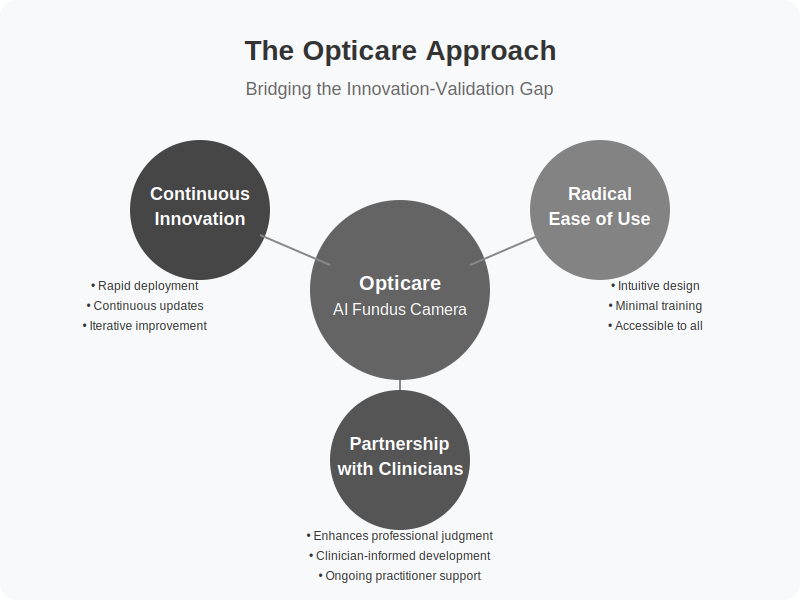
\includegraphics[keepaspectratio]{index.zh_files/mediabag/_resources/images/ch7/opticare-approach-diagram-grayscale.pdf}}

}

\caption{Opticare方法:技术发展快于科学}

\end{figure}%

\textbf{持续创新}

Opticare哲学的核心是对持续创新的承诺。公司坚信,突破性技术应在能够负责任地部署时尽快到达从业者和他们的客户手中,而不是在多年的传统验证周期之后。这一原则认识到,在实施可能有益的技术之前等待完全的科学共识可能会延迟宝贵的护理机会。

这种方法并不意味着将未经证明的技术匆忙推向市场。相反,它涉及对风险-收益概况的仔细评估,特别关注视网膜成像的非侵入性性质。与介入治疗或药物不同,眼底摄影对患者几乎没有直接风险,同时通过早期检测健康模式提供了显著的潜在益处。

Opticare的开发周期强调基于现实世界反馈的快速迭代。新功能不断开发,内部测试,与现有数据集验证,然后小心引入从业者。这种渐进式部署策略允许在保持系统可靠性的同时控制新功能的引入。

持续创新原则延伸到软件更新的管理方式。与可能扰乱既定工作流程的不频繁重大发布不同,Opticare采用滚动更新方法。改进逐步部署,允许从业者逐渐适应,同时在增强功能可用时立即受益。

\textbf{极致易用性}

Opticare方法的第二个核心原则集中于通过极致易用性使先进技术对尽可能广泛的从业者可访问。公司认识到,如果技术过于复杂或在日常实践中使用不便,即使是尖端技术也几乎没有益处。

这一原则体现在优先考虑简单性和可靠性的硬件设计上,而不是技术复杂性。相机的物理界面直观,操作所需的最小培训。自动功能如自我定位和自动对焦调整消除了许多传统上将视网膜成像限制在专业环境中的技术障碍。

软件界面也同样注重易用性设计。报告系统以清晰、可操作的格式呈现复杂信息,支持临床决策而无需广泛的技术知识。与来自不同背景的从业者进行用户体验测试有助于确保系统无论技术专长如何都保持可访问性。

对易用性的承诺不仅限于技术本身,还包括整个实施过程。简化的设置程序、全面但简洁的培训材料和响应迅速的支持系统帮助实践以最小的干扰整合技术。这种方法使先进成像能力民主化,使那些通常缺乏此类技术所需专门资源的实践也能使用。

\textbf{与临床医生的合作}

第三个基本原则认识到,无论技术多么先进,当由知识渊博的医疗专业人员部署时,它才能发挥最高目的。尽管专注于自动化和易用性,Opticare坚持认为临床专长对于适当技术利用仍然至关重要。

这种合作方法意味着开发增强而不是试图取代专业判断的技术。系统提供复杂的分析并识别模式,但从业者根据他们更广泛的临床理解和对个别客户的了解来解释这些发现。

Opticare在整个开发过程中积极寻求执业临床医生的意见。从最初的概念到部署和持续改进,医疗专业人员提供了塑造技术能力和实际实施的关键见解。这种协作方法有助于确保技术解决真实的临床需求,而不是为了技术能力本身而追求。

合作原则还指导Opticare如何处理客户关系。公司不仅仅是提供设备,而是与从业者建立持续的关系,提供继续教育、实施支持和参与未来发展的机会。这种参与帮助实践最大化技术的好处,同时为公司提供持续改进的宝贵反馈。

通过专注于这三个核心原则------持续创新、极致易用性和与临床医生的合作------Opticare方法为在医疗环境中负责任地部署先进技术创造了一个框架。这种平衡的方法允许从业者访问尖端功能,同时保持专业标准和优先考虑客户护理。

随着我们前进,这种方法将继续与技术本身一起进化。新功能将出现,易用性将进一步提高,临床合作将加深。在这一演变过程中,核心原则将保持不变,为视网膜成像技术及其在健康护理中的应用的持续进步提供稳定基础。

\subsection*{现实世界证据的作用}\label{ux73b0ux5b9eux4e16ux754cux8bc1ux636eux7684ux4f5cux7528}
\addcontentsline{toc}{subsection}{现实世界证据的作用}

医学界对证据的方法历来由一个熟悉的金字塔表示。其顶端是系统评价和元分析,其次是随机对照试验(RCT)、队列研究、病例对照研究,最后是基层的专家意见。这一层次结构几十年来为医学服务良好,为评估新治疗和干预措施提供了清晰的框架。然而,像先进视网膜成像系统这样的人工智能医疗设备的出现,要求我们重新想象这一传统结构。

考虑一台配备人工智能分析能力的现代眼底相机。它可能在一天内处理数百张图像,每张图像生成关于图像质量、检测准确性和临床相关性的数据。在一个月内,它可能积累的单个数据点比典型的RCT还多。在一年内,跨多个设备和实践,它可能分析的案例比所有关于传统眼底摄影的已发表研究加起来还要多。这种现实世界证据的量无法整齐地适应传统证据金字塔,但它提供了补充常规研究方法的关键见解。

现实世界证据为技术评估带来了独特的优势。与通常涉及精心挑选的患者群体和标准化条件的控制试验不同,现实世界数据捕捉了临床实践的复杂现实。它展示了技术如何在不同人群、不同临床环境和不同实施方法下的表现。这种经验的广度常常揭示控制研究可能错过的见解。

例如,考虑照明条件对图像质量的影响。控制试验可能标准化照明以确保一致的结果。但现实世界实施数据可能显示,某些照明配置虽然从技术角度看并非最佳,但在繁忙的临床环境中实际上效果更好,因为它们对工作人员来说更实用。这种实用见解只有通过大规模的现实世界使用才能显现。

现实世界证据促成的快速反馈循环也在技术开发中发挥了关键作用。当数百个地点的从业者每天使用系统时,模式很快就会显现。一个使老年患者图像捕获更困难的微妙用户界面问题可能在几周内而不是几个月或几年内在控制研究中显现。这些快速见解使快速迭代和改进成为可能,显著影响临床实用性。

然而,这并不意味着我们应该放弃传统证据层次。相反,我们需要扩展我们对评估现代医疗技术时什么是有效证据的理解。这一扩展框架必须同时容纳传统临床验证和新的技术和实用验证形式。

例如,算法性能指标代表了一个不完全适应传统层次的新证据类别。这些指标可能包括敏感性和特异性测量,但也包括技术参数,如处理速度、各种条件下的错误率和算法随时间稳定性。理解这些指标对于评估人工智能医疗设备至关重要,但它们需要与传统临床措施不同的专长和验证方法。

技术验证研究提供了另一种必不可少的证据形式。这些研究检查算法可重复性、硬件可靠性以及系统在各种操作条件下的稳健性等问题。虽然它们可能不直接测量临床结果,但它们提供了关于系统基本可靠性和可信度的关键信息。

用户体验反馈,在传统证据层次中常被忽视,对于人工智能医疗设备尤为重要。这些系统的有效性不仅取决于其技术能力,还取决于从业者将其成功整合到临床工作流程中的能力。系统收集和分析用户反馈提供了关于现实世界实用性和实际实施挑战的基本证据。

安全监控数据代表了另一个关键的证据类别。现代医疗设备可以包括持续跟踪性能指标、错误率和潜在安全问题的自动监控系统。这种持续监控提供了超越传统临床试验所能提供的安全保证水平,使潜在问题的快速检测和响应成为可能。

挑战在于将这些不同的证据形式整合成一个连贯的技术评估框架。我们需要能够将传统临床证据与技术验证数据、现实世界性能指标和实用实施见解一起权衡的方法。这种综合评估必须考虑的不仅是技术在理想条件下的工作情况,还有它在现实世界临床环境中的表现以及它如何影响整体患者护理。

一种有前景的方法涉及并行证据流。通过控制试验的传统临床验证继续进行,为特定临床应用提供强有力的证据。同时,现实世界证据通过日常使用积累,技术验证确认可靠性和性能,用户反馈通知实用实施。这些流不是竞争,而是互补,每一个都提供了独特的见解,有助于我们理解技术的价值和适当使用。

这种扩展的证据框架特别适合像人工智能视网膜成像这样的技术。视网膜摄影的基本安全性通过数十年的临床使用已经确立。创新在于新的图像捕获和分析方法。对于这些方面,技术验证和现实世界性能数据实际上可能比传统临床试验提供更相关的证据。

随着我们前进,关键在于在承认新证据形式有效性的同时保持科学严谨性。我们必须开发系统的方法来收集和分析现实世界数据,建立技术验证标准,并创建将各种类型证据整合到全面技术评估中的框架。只有通过拥抱这种更广泛的证据观点,我们才能有效地评估和实施迅速发展的医疗技术,这些技术有望改变患者护理。

\section{人工智能的优势}\label{ux4ebaux5de5ux667aux80fdux7684ux4f18ux52bf}

2012年春天,一个深度学习系统因教会自己识别YouTube视频中的猫而登上头条。当时看似琐碎的成就标志着我们处理模式识别方式的根本转变。同样的基础能力------从海量数据中学习复杂模式的能力------现在驱动着包括视网膜检查在内的先进医学影像分析。但其影响远不止简单的模式匹配。

人工智能在医学影像中的核心优势不仅在于其分析图像的能力,还在于它通过规模学习和改进的方式。传统医学图像分析依赖于人类专家应用标准化标准。虽然这种方法非常有效,但它有固有的局限性------人类专家只能检查有限数量的图像,只能记住有限数量的模式,并且只能在有限的时间内保持一致的性能。人工智能系统以超越这些限制的方式创造了它们自己的验证形式。

考虑人工智能系统分析视网膜图像时会发生什么。每处理一张图像都添加到系统的经验数据库中。随着现代眼底相机每天在多个地点捕获数千张图像,人工智能的``经验''以人类专家无法匹敌的速度增长。这种规模创造了传统医疗实践中不存在的学习和验证机会。

现代人工智能系统的持续学习能力代表了与传统医疗设备的根本背离。常规诊断工具一旦校准和部署就保持静态。其性能可能随时间下降,但不会提高。相比之下,人工智能系统可以随着处理的每张新图像、识别的每个新模式和发现的每个新相关性而改进其能力。

这种学习不仅限于简单的模式识别。现代人工智能系统可以识别人类观察者可能看不到的庞大数据集中的微妙关系。它们可以将视网膜结构的细微变化与系统性健康状况相关联,以完美的一致性跟踪随时间的变化,并在不同患者群体中识别新兴模式。这种分析的规模通过纯粹的统计力量提供了一种验证形式。

人工智能分析的一致性提供了另一个关键优势。无论训练多么良好的专家,他们的评估都会显示自然变化。疲劳、分心或简单的人类不一致性都可能影响他们的判断。人工智能系统无论工作量或一天中的时间如何都能保持一致的性能。当追踪随时间变化的微妙变化或比较不同实践的结果时,这种一致性变得尤为有价值。

人工智能分析的可扩展性创造了通过人类审查者难以实现的质量控制机会。每张图像都可以自动检查质量指标,如对焦、照明和定位。异常结果可以标记以供审查。可以通过数千张图像跟踪性能指标,以识别准确性或一致性中的任何漂移。这种自动质量控制提供了通过人类审查实现将成本高昂的验证水平。

也许最重要的是,人工智能系统可以迅速识别不同人群中的模式。传统临床研究常常因地理和物流限制而难以代表人口统计学特征。从多个地点分析图像的人工智能系统可以快速积累不同种族群体、年龄范围和健康状况的数据。这种暴露的多样性有助于验证系统在比典型临床试验所能达到的更广泛人群中的性能。

人工智能分析的规模还使得快速识别罕见病症或异常模式成为可能。虽然人类从业者在其职业生涯中可能只遇到几次罕见的视网膜病症,但每天处理数千张图像的人工智能系统可能在几周内识别出多个例子。这种对罕见病例的加速暴露有助于验证系统识别不寻常表现的能力,同时为未来参考构建有价值的数据库。

然而,规模和人工智能能力的优势必须与仔细验证底层算法的需求相平衡。处理数百万张图像的能力并不自动保证准确分析。关键在于将人工智能的可扩展能力与确保可靠性和临床相关性的严格验证协议相结合。

这种验证采取多种形式。技术验证通过使用已知结果的控制测试确认人工智能的基本模式识别能力。临床验证验证这些能力转化为有意义的诊断见解。现实世界验证确保系统在不同实践环境和患者群体中一致表现。

人工智能系统的快速适应能力为验证创造了机会和挑战。虽然系统可以快速纳入新信息并提高其性能,但这种适应性需要仔细监控,以确保变化增强而不是降低临床实用性。这导致了专为适应性人工智能系统设计的新验证协议的开发。

自动监控系统在持续验证中发挥了关键作用。这些系统跨数百万次分析跟踪性能指标,识别任何偏离预期模式的偏差。它们可以检测系统性能的微妙变化,这可能表明需要调整或揭示值得调查的新模式。这种持续监控提供了与人工智能系统适应性相匹配的动态验证形式。

展望未来,人工智能在医学影像中的优势可能会变得更加显著。计算机视觉、机器学习和数据分析的进步继续增强这些系统能够识别和理解的内容。挑战不在于开发这些能力,而在于负责任地验证它们并在临床实践中有效实施。

人工智能分析的规模并没有取代传统验证方法,而是提供了帮助弥合创新-验证差距的补充证据。通过将人工智能的可扩展能力与严格的验证协议相结合,我们可以利用机器学习的力量,同时保持最高标准的临床护理。这种平衡的方法使我们能够推进医学影像技术,同时确保它服务于其最终目的------改善患者护理和结果。

\section{结论}\label{ux7ed3ux8bba-2}

技术进步的快速步伐为健康从业者带来了机遇和挑战。虽然传统科学验证仍然重要,但理解和适当地实施新技术需要一种平衡的方法,考虑经典证据和现代验证方法。

成功在于在拥抱创新增强客户护理潜力的同时保持专业标准。这需要持续教育、谨慎实施和对道德实践的承诺。

未来健康护理将越来越多地涉及像Opticare人工智能相机这样的技术增强工具。理解这些工具的能力和局限性,同时保持适当专业边界的从业者,将最有能力为客户提供最佳护理。

关键要点:

\begin{enumerate}
\def\labelenumi{\arabic{enumi}.}
\tightlist
\item
  技术往往比传统验证发展更快
\item
  多种形式的证据支持技术创新
\item
  专业责任需要平衡实施
\item
  持续教育和适应至关重要
\item
  清晰的沟通和记录仍然至关重要
\item
  道德实践指导技术采用
\end{enumerate}

通过理解这些原则并深思熟虑地实施它们,从业者可以成功导航技术增强健康护理的不断发展的景观。

\bookmarksetup{startatroot}

\chapter{视网膜成像与人工智能的未来}\label{ux89c6ux7f51ux819cux6210ux50cfux4e0eux4ebaux5de5ux667aux80fdux7684ux672aux6765}

\section{引言}\label{ux5f15ux8a00-1}

视网膜成像领域正站在巨大进步的门槛上,这一进步由人工智能、成像技术和数据分析的快速发展所驱动。本章探讨新兴趋势和潜在的未来发展,同时保持对这些发展对健康从业者影响的实际关注。

\section{当前技术状态}\label{ux5f53ux524dux6280ux672fux72b6ux6001}

\subsection*{今日能力}\label{ux4ecaux65e5ux80fdux529b}
\addcontentsline{toc}{subsection}{今日能力}

Opticare AI 相机代表了当前视网膜成像技术的水平:

\begin{itemize}
\tightlist
\item
  1200万像素分辨率
\item
  40度视野角
\item
  最小2.8毫米瞳孔直径要求
\item
  非散瞳成像
\item
  AI驱动分析
\item
  便携设计
\item
  快速结果交付
\end{itemize}

\subsection*{基准性能指标}\label{ux57faux51c6ux6027ux80fdux6307ux6807}
\addcontentsline{toc}{subsection}{基准性能指标}

\begin{itemize}
\tightlist
\item
  图像捕获时间:5分钟以内
\item
  分析交付:近实时
\item
  便携性:总重量2千克
\item
  连接性:标准USB和HDMI
\item
  电源要求:标准插座连接
\end{itemize}

\section{新兴技术}\label{ux65b0ux5174ux6280ux672f}

先进光学技术与人工智能的融合正准备彻底改变我们通过视网膜检查理解人类健康的方式。展望未来,几项关键技术发展有望增强视网膜图像的捕获和分析能力,为整体健康模式提供越来越复杂的见解。

\textbf{推进图像捕获艺术}

有效视网膜分析的基础始于图像质量。下一代成像系统可能将整合多光谱能力,超越传统可见光摄影,以捕获跨越更宽波长范围的信息。这种更广泛的光谱分析有望揭示当前系统可能遗漏的微妙组织变化。通过检查不同波长如何与视网膜组织相互作用,这些先进系统可以提供关于组织组成和健康模式的更详细信息。

高分辨率传感器技术在数字成像更广泛发展的推动下继续快速进步。未来的视网膜相机可能会具有显著增加的像素密度,能够捕获当前系统无法解析的微观细节。这种增强的分辨率可能揭示视网膜结构的微妙变化,提供潜在健康变化的更早期指示。改进的传感器技术也承诺在挑战性条件下提供更好的性能,例如检查小瞳孔患者或处理眼球运动。

广角成像技术代表另一个有前途的前沿领域。未来系统可能在单次曝光中捕获越来越全面的视网膜视图,减少检查时间同时提供更完整的文档记录。这种扩展的视野对于追踪随时间推移的微妙变化可能特别有价值,因为它确保了对否则可能被忽视的周边区域的一致覆盖。

\textbf{AI革命继续}

未来视网膜成像系统的真正力量在于其分析能力。先进的AI算法可能会以前所未有的速度和准确性处理这些增强图像。经过不断扩大数据集训练的深度学习模型将识别越来越微妙的模式和变化。这些系统可能超越简单的模式匹配,理解不同视网膜特征之间的复杂相互关系及其对健康的潜在影响。

实时分析能力将改变成像过程本身。未来系统可能不再是捕获图像后等待处理,而是提供关于图像质量和潜在关注区域的即时反馈。成像系统与操作者之间的这种动态交互可以确保最佳结果,同时减少重复捕获的需求。系统可能会根据对捕获条件的实时分析指导操作者调整定位或设置。

\textbf{隐私和安全创新}

随着这些系统变得更加复杂,在推进分析能力的同时保护患者隐私变得越来越重要。联邦学习方法提供了一个有前途的解决方案,允许AI模型从分布式数据集学习,而无需集中敏感的患者信息。这项技术可以实现分析能力的持续改进,同时维持强大的隐私保护。

\textbf{集成和互操作性}

未来系统可能会与其他健康评估工具无缝集成,创建个体健康模式的更全面视图。这可能包括与基因信息、生物标志物数据和生活方式因素的整合,以提供更具上下文的见解。将视网膜模式与其他健康指标相关联的能力可以增强我们对各种因素如何影响整体健康的理解。

\textbf{增强可视化和沟通}

先进的可视化技术将改变从业者和患者如何与视网膜成像结果交互。三维建模可以提供理解视网膜结构及其随时间变化的直观方式。交互式显示可能允许从业者探索视网膜的不同层次和方面,增强他们向患者解释发现的能力。

人工智能可能在生成清晰、易于理解的报告方面发挥越来越重要的作用,帮助从业者有效地传达发现。这些报告可能自动适应不同受众的需求,为医疗服务提供者提供技术细节,同时为患者提供清晰易懂的摘要。

\textbf{扩展应用}

随着这些技术的成熟,它们的应用可能会超越当前用途。增强的成像和分析能力可能揭示视网膜特征与整体健康之间的新模式和关系。这可能导致对潜在健康变化的更早识别,允许更主动的健康方法。

移动和远程筛查能力可能会显著扩展。先进的便携系统可能将复杂的视网膜成像带到服务不足的地区,或在非传统环境中实现便捷筛查。这可能使先进健康筛查工具的获取民主化,同时生成有价值的数据以进一步改进分析能力。

\section{视网膜成像的硬件演变}\label{ux89c6ux7f51ux819cux6210ux50cfux7684ux786cux4ef6ux6f14ux53d8}

未来十年有望在视网膜成像硬件方面取得重大进展,这些进展由光学技术、电子微型化和材料科学等领域的更广泛发展所驱动。这些进步可能彻底改变视网膜成像在健康实践中的实际应用。

\textbf{微型化和便携性}

当前的视网膜相机与传统眼科设备相比已经紧凑,但这仅仅是微型化可能性的开始。新兴的半导体技术和先进制造工艺可能实现显著更小的成像系统,而不会牺牲图像质量。这些更小的设备可能接近当前智能手机相机的尺寸,同时保持专业级的成像能力。

这种尺寸减小带来的实际好处不仅仅是便利。更小的设备在实践环境中需要更少的专用空间,提供更灵活的部署选项。增强的便携性将使移动筛查服务变得更加实用,允许从业者在各种环境中直接将这项技术带给客户。

电池技术的演变,由电动汽车开发和移动电子设备推动,将支持这些便携系统。新电池化学技术承诺更高的能量密度和更快的充电速度,实现长时间移动操作而无需频繁充电。这种增强的移动性可能彻底改变从业者如何将视网膜成像整合到他们的服务中。

\textbf{光学进步}

光学技术的发展可能在提高图像质量的同时减少系统复杂性。新的镜头材料和设计,包括金属镜头和自适应光学,可能实现更好的光线管理和减少像差。这些进步可以提高图像质量,同时可能减少设备尺寸和重量。

LED技术的改进将增强照明能力。更高效、精确控制的光源将实现更好的图像捕获,同时保持患者舒适度。先进的光谱控制可能允许同时在多个波长捕获,提供关于视网膜组织的更丰富数据。

对焦系统可能变得更加复杂,同时需要更少的机械复杂性。使用液体镜头或类似技术的电子对焦调整可能取代传统机械系统,提高可靠性同时减少设备尺寸。这些系统也可能实现更快、更精确的对焦,改善图像质量和检查效率。

\textbf{集成和连接性}

未来设备可能提供增强的连接选项,支持与实践管理系统和其他健康评估工具的无缝集成。无线数据传输将成为标准,消除电缆连接同时保持数据安全。这种改进的连接性可能实现在需要时与同事或专家的实时咨询。

云集成可能变得更加复杂,提供自动备份和同步能力。增强的安全功能将保护患者隐私,同时实现护理提供者之间适当的数据共享。这些系统也可能支持自动软件更新和远程诊断,简化设备维护。

移动设备集成可能会显著扩展。未来系统可能使用平板电脑或智能手机作为控制界面和初步查看屏幕,减少系统复杂性同时提高可用性。这种方法也可以通过利用熟悉的技术简化培训并减少成本。

\textbf{制造和材料}

先进的制造技术,包括改进的精密模塑和光学组件的3D打印,可能在保持质量的同时降低生产成本。新材料可能提供更好的耐久性和热稳定性,同时减轻重量。这些改进可能使先进的视网膜成像对更广泛的从业者更加可及。

模块化设计方法可能实现更容易的升级和维护,延长设备寿命同时降低长期成本。组件可以单独更换或升级,而不需要完全更换系统,支持更可持续的实践投资。

\textbf{实际影响}

这些硬件进步可能彻底改变从业者如何在他们的实践中实施视网膜成像。更便携、更稳健的设备将实现灵活的部署选项,支持传统办公环境和移动服务。改进的可用性和减少的维护需求将帮助从业者专注于客户护理而非技术操作。

增强的图像质量和自动优化功能可能提高检查效率同时保持准确性。实时质量评估和引导功能可以减少重复捕获的需要,同时提高从业者效率和客户体验。

随着这些硬件进步的继续,从业者应该为可用技术的持续演变做好准备。成功将需要平衡新能力的好处与实际实施考虑。了解这些趋势有助于为技术投资决策提供信息,同时保持对可持续实践发展的关注。

关键在于不是为了技术本身而追求最新技术,而是深思熟虑地选择能够增强实践能力同时支持客户护理目标的工具。通过了解硬件演变并保持这种实际视角,从业者可以有效地利用先进技术支持他们的实践目标。

\section{软件发展}\label{ux8f6fux4ef6ux53d1ux5c55}

明天的视网膜成像不仅承诺更好的硬件,还将从根本上改变从业者如何提取、解释和利用隐藏在眼睛中的见解。这些转变同时在多个领域酝酿。

分析算法每天变得越来越复杂,很快将以前所未有的速度处理图像,同时从视网膜模式中提取以前不可见的信息。这些先进系统不再仅限于检测明显的异常,将揭示微妙的组织特征及其与整体健康的复杂关系。曾经需要几分钟的过程可能在几秒钟内完成;曾经需要专家解释的内容可能立即对普通从业者可用。

机器学习------这场正在重塑医疗保健的安静革命------准备显著增强视网膜分析中的模式识别能力。这些系统不仅仅匹配人类能力;它们将超越人类。通过识别即使经验丰富的临床医生也看不到的微妙变化,同时通过上下文理解减少假阳性,AI驱动的工具将变得越来越不可或缺的健康评估伙伴。它们的准确性,已经令人印象深刻,将随着分析更多数据而进一步提高,从每个处理的新图像中学习。

我们如何看待和理解视网膜本身将通过革命性的可视化工具进化。想象一下探索视网膜结构的三维模型,从任何角度旋转和检查它们。考虑当增强对比度和过滤选项揭示以前隐藏的细节时的可能性。这些进步不仅仅有助于诊断,它们将彻底改变从业者如何理解和向同事及客户传达他们的观察。

一刀切的界面时代已经结束。明天的系统将适应从业者,而不是强迫从业者适应它们。可定制的显示将允许专业人员优先显示与其独特实践方法最相关的信息。想强调血管模式?更喜欢专注于神经组织评估?选择权在你手中,提高工作流程效率而不牺牲对全面数据的访问。

触摸屏幕,放大感兴趣区域,滑动比较随时间变化的图像------交互式功能将彻底改变从业者如何探索和解释视网膜发现。复杂分析将不再需要复杂界面。相反,通过不同图像层或分析选项的直观导航将使复杂评估对各专业的从业者都可访问,显著提高他们以清晰易懂的方式向客户解释发现的能力。

自动化将悄然改变日常工作流程。想象一个系统,根据客户的独特特征建议最佳捕获设置,或自动标记需要仔细检查的区域。这些智能助手将处理常规任务,同时保留专业监督,同时提高效率并确保各检查间的一致质量。

``上个月我在哪里看到过那种不寻常的血管模式?''这类问题将通过复杂的信息组织系统立即找到答案。增强的搜索能力将让从业者在几秒钟内定位相关信息,支持个人护理决策和跨患者群体的更广泛模式分析。费力审查数十份记录的日子将让位于即时、智能的数据检索。

客户隐私------始终是首要考虑------将受益于不断发展的安全功能。先进的加密和精细访问控制将为从业者提供所需的灵活性,以保持严格的保密性,同时实现与其他专业人员的适当协作。这些系统将在现代医疗保健所需的保护与可访问性之间取得微妙平衡。

数据丢失的噩梦将成为过去的遗物。自动备份系统将默默保护每个图像和分析,而云集成提供安全、随处可访问的存储。系统更新将在非工作时间自动安装,优化性能而不中断实践操作。这些看似平凡的功能将显著减少管理负担,同时确保数据保持安全和可访问。

实践管理将通过视网膜成像系统与其他临床工具之间的无缝集成而转变。患者信息将在系统之间毫不费力地流动,同时保持数据完整性。不再需要手动数据输入,不再有信息孤岛------只有由高效信息交换支持的全面、互连的客户护理。

报告将以非凡的灵活性适应其受众。需要专家咨询的技术分析?点击生成。想要一个清晰、易于理解的客户教育摘要?同一系统将同时生成两者,自动调整内容和复杂性以适应预期接收者。这些自适应报告功能将增强沟通,同时在不同受众中保持专业标准。

办公室本身将对实践管理的许多方面变得可选。移动访问能力将显著扩展,允许通过智能手机、平板电脑或笔记本电脑安全地查看数据。从业者可能从家中检查令人关注的发现,或在旅行时查看进度报告。这种灵活性将同时支持实践管理和客户护理,尽管保持适当的安全措施仍然至关重要。

``这个图像质量足够好吗?''这个问题将通过高级质量控制功能自行回答,这些功能在捕获过程中提供实时反馈,同时自动记录评估质量。这些能力将毫不费力地维持专业标准,支持实践效率,同时确保每个图像都达到最佳诊断标准。

也许最令人兴奋的是,模式跟踪能力将演变为揭示随时间变化的微妙故事。增强的时间变化可视化可能揭示在单次检查中不可见的趋势,支持真正主动的健康方法。这些纵向见解将显著增强定期监测的价值,将定期检查转变为强大的预测工具。

随着这些非凡能力的出现,从业者必须保持对基本目标的明确关注。成功需要在拥抱新功能和确保它们真正支持临床目标之间的深思熟虑平衡。了解这些趋势不是为了追求技术本身,而是为了做出保持对客户护理强调的明智决定,同时增强实践能力。

关键?选择真正增强实践能力同时支持专业标准的工具。通过保持这种实际视角并了解软件演变,从业者可以利用先进技术支持有意义的实践目标,而不被新奇性或复杂性分心。

视网膜成像软件的未来闪烁着希望。但实现这一希望需要的不仅仅是安装和更新------它需要专注于实际益处而非技术复杂性的深思熟虑实施。随着这些工具继续快速演变,从业者应该为持续进步做好准备,同时永远不要忘记其主要目的:支持杰出的客户护理。

\section{临床应用}\label{ux4e34ux5e8aux5e94ux7528}

当尖端技术遇到实际健康护理会发生什么?随着视网膜成像的发展,从业者站在如何理解和支持客户健康的显著转变门槛上。这不是遥远的未来------这些变化正在展开,创造前所未有的机会增强护理,同时尊重关键的专业边界。

想象集成的力量。不再局限于孤立检查视网膜模式,明天的从业者将这些观察与其他健康标志的星座相关联。血液检测、基因评估、生活方式因素------所有这些与视网膜发现编织在一起,创建比任何单一指标能提供的更丰富的理解。这种全面方法不会扩大实践范围;相反,它将在现有专业边界内深化护理影响。

时间揭示单一时刻无法显示的内容。先进的时间分析将彻底改变模式跟踪,系统能够自动检测即使最敏锐的眼睛也看不到的微妙变化。三个月前是否出现过那种血管模式?色素沉着的微妙变化是否进展?复杂的比较工具将立即回答这些问题,实现真正主动的健康方法,在问题形成前发现趋势。

上下文将数据转化为智慧。通过将个体模式与更广泛的人口指标比较------同时保持严格的隐私保护------从业者将获得对其观察的前所未有的视角。这种变异对于这个年龄和背景的人来说是否常见?它与通常与最佳健康相关的模式相比如何?这种上下文理解不仅仅满足好奇心;它将显著增强建议质量,同时保持坚定的专业范围。

技术理解与客户理解之间的差距将通过先进的可视化工具显著缩小。交互式显示将抽象医学概念转化为直观、可探索的体验。曾经对他们几乎不理解的解释礼貌点头的客户将转而积极参与发现自己的健康模式。``展示,而非仅告知''将随着从业者引导客户通过视觉旅程照亮、教育和激励而获得新含义------所有这些都在保持适当专业边界的同时进行。

教育将精确适应个人需求。通用的小册子和一刀切的解释已成过去。相反,系统将生成定制资源,直接针对每个客户的具体发现、问题和学习风格。这些个性化材料------也许特色展示客户自己的视网膜图像以及清晰解释------将弥合临床见解与个人理解之间的差距,通过理解而非指令培养合规性。

检查本身将通过实时可视化转变。当图像即时出现在屏幕上,从业者可以立即优化捕获技术,而客户则目睹自己的内部景观在眼前展开。这种共享体验创造了教育的自然机会,问题自然从观察而非抽象讨论中产生。技术质量提高,客户参与加深,有意义健康对话的基础在一个优雅过程中凝固。

随着自动化进步,管理将退居幕后。实践工作流程,曾经由文档和调度挑战主导,将变得非常精简。系统将自动记录发现,根据观察到的模式建议适当的跟进间隔,甚至为从业者审核生成初步建议。这种效率并不削弱从业者的角色------它提升了这一角色,为不可替代的人类元素------解释、连接和个性化指导------创造空间。

质量保证,曾经需要警惕关注和艰苦审查,将变得既更复杂又更易于实施。自动系统将悄然确保文档符合专业标准,验证图像质量,并在不同从业者之间保持一致性。这位卓越的无形守护者在不增加管理负担的情况下支持实践效率和护理质量。

客户关系将加深,即使管理工具简化。全面而直观的系统将增强从预约安排到访问间沟通的一切,减少行政摩擦同时加强个人连接。这种悖论美丽地解决:随着技术处理客户管理的机制,从业者获得自由专注于技术永远无法替代的护理人类维度。

距离将不再是优质护理的障碍。远程咨询能力,由先进成像和安全通信工具支持,将把专家指导带给不分地点的客户。农村地区、行动受限或只是面临繁忙日程的人将获得以前无法获取的护理。实践将服务更多客户而不牺牲质量,扩展其影响同时保持其护理方法的完整性。

社区参与将通过增强的移动性扩展。便携、自动化系统将把停车场变成筛查中心,社区大厅变成健康诊所,工作场所休息室变成健康评估站。从业者将把复杂能力直接带到人们生活、工作和聚会的地方,保持专业标准同时显著扩展可及性。

专业化将与通识化一起蓬勃发展。随着对视网膜模式理解的深化,一些从业者将在特定应用中发展专注专长------也许是心血管健康、代谢功能或认知健康。这些专业评估项目将为特定客户需求提供增强价值,同时保持适当范围,通过差异化而非边界扩张创造新的实践机会。

这些进步中没有一项减少了专业发展的重要性------恰恰相反。成功使用越来越复杂的工具需要持续教育和培训。繁荣的从业者将是那些了解新兴技术同时保持对实际应用不懈关注的人,确保技术服务于其实践目标而非指导它们。

协作护理将达到无缝协调的新水平。在保持不同学科之间适当边界的同时,从业者将更容易与其他健康专业人员共享相关信息。有营养师、体能教练和心理健康顾问的客户将体验到一种协调方法,每个提供者都了解其他人的见解和建议。这些增强的连接支持真正全面的护理,同时尊重不同的专业角色。

通过先进视网膜成像转变健康实践的潜力光芒四射,但实现这一潜力需要平衡。成功需要深思熟虑地整合新工具,同时保持对客户护理和专业标准的坚定关注。通过了解新兴能力并保持这种平衡视角,从业者可以有效地利用技术支持------而非取代------其核心实践目标。

重要的不是技术复杂性,而是对护理能力的实际增强。最先进的系统如果不能有意义地改善客户结果或实践效果,提供的价值很小。通过仔细规划和持续适应,从业者可以建立更强大、更有效的实践,同时保持客户健康在每个决策的中心。

随着技术进步,实践本身必须演变。客户护理和实践管理的方法将需要深思熟虑的重新校准,以保持在拥抱新工具和确保实际价值之间的平衡。这不是追逐趋势;而是确保每项技术投资真正支持实践成功,同时维护专业标准。

在所有这些演变中,客户需求必须保持核心考虑。每项技术进步都应通过简单镜头评估:这如何增强客户护理同时保持个人连接?这种以客户为中心的视角为导航技术决策提供指南,同时建立不仅技术先进,而且在支持人类健康方面真正有效的实践。

\section{数据分析与研究}\label{ux6570ux636eux5206ux6790ux4e0eux7814ux7a76}

站在先进成像、人工智能和大数据分析的交叉点,你将见证健康评估领域的一场彻底革命。这种强大的融合不仅改变了我们在视网膜中所见的内容,还从根本上转变了我们理解这些精细结构与整体健康之间复杂关系的方式。对于具有前瞻性思维的从业者来说,这些发展提供了前所未有的机会来增强研究和实际应用,同时保持基本的专业边界。

数据爆炸即将来临。随着视网膜成像成为全球健康实践的标准组成部分,收集信息的绝对量将超出以往任何可想象的规模。过去研究人员为有限样本量而挣扎,先进分析系统将很快筛选数百万张图像,识别肉眼看不见的微妙模式。这些系统不会损害个人隐私;复杂的匿名化技术将保护个人信息,同时允许模式本身发声。从这片浩瀚的数据海洋中将出现以前未被认识的关系------特定视网膜特征与各种健康方面之间的联系,这些联系至今仍然隐藏。

协作不必意味着集中化。联邦学习方法------健康研究中的革命性概念------将使全球各地的实践能够在不共享敏感客户数据的情况下为集体知识做出贡献。想象一个系统,你的实践的AI从本地模式中学习,然后只与全球模型共享这些抽象见解。这种分布式方法极大地加速了我们对视网膜模式的理解,同时对机密信息保持铁壁般的保护。隐私和进步携手并进。

时间揭示单一时刻所隐藏的内容。纵向数据------跟踪同一个体数月乃至数年------的真正力量怎么强调都不为过。随着我们积累这些延伸的健康叙事,我们将获得对视网膜模式如何随时间演变的前所未有的洞察。这些时间性指纹可能揭示各种健康趋势的早期指标,远在它们在其他地方表现出来之前,实现真正主动的健康维护策略。个人护理和人口层面的理解都将通过这些延伸的观察而进步。

人工智能随着分析的每一张图像变得更加敏锐。在不断扩大的数据集上训练的机器学习模型将很快识别出即使经验丰富的人类观察者也可能错过的视网膜结构中的细微变化。血管弯曲度的微妙变化,色素沉着的微不可察的改变------这些潜在健康变化的细微信号将成为先进AI系统的明确信号。更早的识别意味着更早的干预,同时保持适当的专业边界。

计算机视觉站在显著转型的边缘。这些技术在未来几年将显著进步,实现对视网膜结构前所未有的详细和准确分析。增强的图像处理算法将揭示当前系统无法看见的组织特征,而测量精度将提高数个数量级。这些能力解锁对视网膜特征与更广泛健康模式之间复杂关系的新见解。

预测,而非仅仅检测,代表下一个前沿。通过分析数千或数百万个体的模式,先进分析系统将识别潜在健康变化的早期指标,在它们表现为明显症状之前。这种向预测性健康------在问题发展前识别潜在问题------的转变改变了健康维护的整个范式。从业者将基于这些见解实施主动策略,同时坚定地保持在适当的专业范围内。

一刀切的方法将让位于个性化风险评估。考虑个体特征、历史和独特模式的模型将为每个客户提供量身定制的分析。武装这种个性化智能,从业者可以开发精确匹配特定需求的有针对性健康建议。多种数据源------从视网膜成像到其他健康指标------将无缝整合,增强预测准确性,同时支持真正全面的护理方法。

研究方法学本身面临颠覆。大规模视网膜成像数据的可用性将从根本上改变研究人员如何处理健康问题。传统研究可能包括数十或数百名参与者,未来分析将纳入数十万甚至数百万匿名数据集。通过应用于这些庞大集合的先进统计技术,研究人员将识别重新定义我们对视网膜特征如何连接整体健康理解的模式和关系。

标准从复杂中创造连贯。标准化分析协议将出现,提高研究可靠性,同时促进跨学科和跨边界的协作。共同的测量方法和统一质量标准将使在不同环境中进行的研究之间能够进行有意义的比较。这种和谐化以指数方式加速知识发展,同时保持真正进步所必需的科学严谨。

质量保证通过先进分析变得既更严格又更不繁重。自动系统将持续评估图像捕获的技术方面------焦点、照明、定位------同时确保文档满足完整性标准。这些能力在不增加管理负担的情况下维持专业卓越,提高实践效率同时维持质量标准。

效果以新方式变得可衡量。通过复杂数据分析增强的结果跟踪将为从业者提供清晰见解,了解哪些方法产生结果,哪些需要改进。这些效果的客观衡量识别改进机会,同时确认成功策略,支持持续实践发展,同时不失对最终目标的关注:卓越的客户护理。

这一切都离不开对数据基础的细致关注。成功使用先进分析需要对数据质量和一致性的坚定承诺。聪明的从业者将建立明确协议,管理其数据生态系统的每个方面------从收集方法到存储参数再到访问控制。这种结构化方法确保分析建立在可靠基础上,同时保护措施在每一步都保障客户隐私。

不整合的系统失败,无论其各自的力量如何。随着分析能力的进步,它们与现有实践管理系统的整合变得越来越关键。从业者必须在实施前仔细考虑新分析工具如何与已建立的工作流程保持一致。深思熟虑的整合最大化益处,同时最小化干扰,为从业者和客户创造无缝体验。

对可能性的兴奋必须与清醒的专业精神保持平衡。分析能力的演变为健康实践提供了非凡潜力,但从业者必须在利用这些先进工具的同时保持适当边界。成功取决于找到技术能力增强------而非超出------客户护理实际应用的最佳点。

数据共享带来机遇和义务。随着分析系统变得更加强大,从业者面临着关于信息如何在其实践内外流动的日益复杂决定。理解适当共享的潜在益处和隐私保护的伦理要求变得至关重要。清晰、透明的政策确保数据服务于客户利益,同时尊重保密的基本权利。

适应,而非采用,定义了在这一快速演变的景观中的成功。随着分析能力继续进步------有时以惊人的速度------从业者必须为可用工具和见解的持续演变做好准备。那些繁荣的人将保持对实际应用的不懈关注,同时了解新兴能力,确保技术支持而非指导其实践发展。

地平线闪烁着可能性。未来对视网膜模式及其与健康关系的理解承诺着我们今天几乎无法想象的见解。通过深思熟虑地参与先进分析能力,同时保持坚定的专业标准,从业者可以显著增强其支持客户健康的能力,同时为人类对健康本身的更广泛理解做出贡献。

\section{专业影响}\label{ux4e13ux4e1aux5f71ux54cd}

转变即将来临,健康从业者正处于变革的边缘。随着视网膜成像技术快速发展,实践不仅仅是采用新设备------它们将在其基本运作、客户关系和专业能力方面经历深刻的转变。这种演变呈现出一把双刃剑:提升护理的前所未有机会与需要深思熟虑导航的重大挑战并存。

日常实践运作站在重塑的门槛上。手动图像捕获和费力分析的日子已经过去;明天带来的是智能自动化,以非凡效率处理这些技术方面。想象一下,花更少时间与设备搏斗,更多时间进行有意义的客户互动。想象自己专注于解释结果和制定个性化建议,而不是因技术问题重复捕获。增强的质量控制功能将默默确保每个图像都符合专业标准,减少重拍同时生成一致、全面的文档。

工作流程,曾经僵硬且劳动密集,将流动带有直观智能。智能调度系统将分析视网膜模式,自动提出适当的跟进时间表------对于显示早期血管变化的客户为六周,对于模式稳定的另一位为三个月。集成通信工具将简化从预约提醒到结果通知的一切,减少曾经每天消耗数小时的管理负担。这些相互连接的自动化功能不仅仅节省时间;它们将实践组织转变为从业者和客户的无缝体验。

数据管理------这一必要但常常繁重的责任------将矛盾地变得既更复杂又更简单处理。基于云的系统将安全存储每个图像和分析,自动备份关键信息,同时实现授权护理提供者之间的适当共享。不再需要翻阅文件或与兼容性问题搏斗。相反,增强的搜索和分析工具将帮助你以前所未有的便捷识别客户群体中的模式。这些能力不仅仅组织信息;它们将原始数据转化为可行见解,为个人护理决策和更广泛的实践发展策略提供信息。

客户体验本身将通过先进可视化工具经历戏剧性增强。不再是使用静态图像和技术语言费力解释复杂视网膜模式,你将与客户互动,使用交互式显示使这些概念立即可理解。``看看自上次访问以来血管模式如何变化?''你会说,在客户能清晰理解的屏幕上切换时间点。这种增强的视觉沟通不仅仅满足好奇心------它将从根本上改变客户参与,并显著提高对健康建议的遵守度。

距离将不再是优质护理的障碍。远程咨询能力将扩展服务可及性,而不牺牲有效健康实践所必需的个人联系。想象一下与住在两小时车程外的客户审查结果,使用安全视频连接讨论发现并回答问题,就像你们面对面坐在一起一样。这些能力对于常规跟进和偏远地区客户特别有价值,帮助你的实践扩展其地理范围,同时保持区分卓越护理的关系质量。

客户教育将从通用讲义发展为复杂、个性化体验。自动系统将分析检查发现,生成定制教育内容,针对每个客户的特定模式和健康机会。不再是用一般信息轰炸客户,你将提供精确目标资源,直接关联到他们的独特情况。这种增强方法不仅仅传递信息------它将转变理解,提高客户参与,同时通过知情参与健康旅程支持实质性更好的结果。

你的专业技能将需要深思熟虑的扩展,以利用这些不断进步的能力。除了学习按钮序列或软件界面外,你将需要更深入理解如何解释越来越复杂的分析结果,同时保持适当的专业边界。哪些模式需要立即关注?哪些变化在正常参数范围内?何时应该转介给医学专家?持续专业发展将更少关注基本技术操作,更多关注以增强而非替代你的专业判断的方式将这些强大能力与传统健康方法整合。

跨学科协作将随着信息共享变得更加无缝而蓬勃发展。曾经特征化健康服务的碎片化护理将让位于协调方法,从业者可以轻松与其他健康专业人员和医疗保健提供者共享相关信息。想象一下为同时看你和营养师的客户协调护理,每个专业人员都能适当访问对方评估的相关发现。这些增强连接不会扩大你的实践范围;相反,它们将在你的专业角色内深化你的影响,同时支持真正全面的客户护理。

差异化机会将通过这一强大技术的专门应用出现。一些从业者将专注于视网膜模式提供特别有价值见解的特定健康领域------可能是心血管健康评估、代谢功能监测或早期认知健康筛查。通过在特定应用中发展专业专长,你可以区分你的实践,同时以卓越深度服务特定客户需求。这种专业化不需要扩展超出适当边界;相反,它允许你在已建立的专业范围内最大化影响。

随着这些能力的进步,健康实践的经济方程将发生显著变化。是的,新技术的初始投资需要仔细考虑资本支出与潜在回报的关系。然而,当你考虑到改进的运营效率和增强的服务能力时,数学变得令人信服。许多从业者将通过专业评估服务或移动筛查项目发现以前不可行的新收入机会。具有前瞻性思维的从业者看到的不仅仅是初始价格标签,还有这些能力实现的长期实践增长。

运营成本,曾经变化无常且有时不可预测,将随着系统变得更可靠且维护需求减少而稳定下来。基于云的服务将减少或消除昂贵的IT基础设施需求,同时提供随你的实践增长的可扩展解决方案。这些变化不仅仅帮助你保持财务稳定;它们创造了投资新兴能力的灵活基础,确保你的实践保持在健康护理的前沿。

在这个不断演变的景观中导航成功需要谨慎平衡。不加区别地拥抱每一项新技术能力而不评估其实际价值的从业者会发现自己被功能淹没但结果平平。相反,那些完全抵制技术进步的人将越来越发现自己处于竞争劣势。最佳方法在于深思熟虑的评估:这一特定技术如何与你的实践目标和客户需求保持一致?这种经过衡量的视角确保技术投资真正支持实践成功,同时保持构成你基础的专业标准。

在所有这些技术进步中,一项原则仍然至高无上:客户需求必须保持核心地位。每个实施决定都应始于一个简单问题:这将如何增强客户护理同时保持个人联系?创造从业者与客户之间障碍的技术------无论其能力多么复杂------都未能通过健康实践的基本测试。这种以客户为中心的视角为导航技术决策提供指南,同时建立一个利用进步而不牺牲人性的实践。

健康实践的未来闪烁着可能性------越来越受技术支持,却仍然基本专注于客户护理。这个新景观中的成功既不需要盲目拥抱每一项创新,也不需要顽固抵抗变化,而是需要深思熟虑地整合先进能力,同时保持对专业标准和个人联系的坚定承诺。通过了解新兴技术并保持这种平衡视角,具有前瞻性思维的从业者可以有效适应不断演变的机会,同时保持健康护理的本质。

前进的道路不是为了技术本身而追求技术。它是关于深思熟虑地选择真正增强实践能力同时支持客户护理目标的工具。通过仔细规划和持续适应,从业者可以利用新兴技术建立更强大、更有效的实践------不是通过替代定义健康护理的人类元素,而是通过扩展能力的工具增强它们,同时保持对基本目标的关注:通过知情、富有同情心的指导支持客户健康。

\section{结论}\label{ux7ed3ux8bba-3}

尽管这些发展令人鼓舞,但几个挑战需要仔细考虑。确保AI驱动分析的可靠性和有效性仍然至关重要。随着系统变得更加复杂,保持对其能力和局限性的透明度变得越来越重要。从业者必须了解这些不断发展的技术,同时保持适当的专业边界。

监管环境可能会随着这些技术进步而演变。从业者应该为不断变化的要求做好准备,同时确保其技术使用符合专业标准和道德准则。

视网膜成像技术与人工智能的融合为健康从业者提供了变革性机会。然而,实现这些益处需要深思熟虑如何整合先进能力,同时保持对客户护理和专业标准的关注。

在这个不断演变的景观中取得成功始于对技术采用的平衡方法。从业者应该根据其实践需求和客户要求仔细评估新能力,避免仅仅因为新功能或升级存在而拥抱它们的诱惑。这种经过衡量的方法有助于确保技术服务于实践目标而非驱动它们。

实施过程需要仔细的时机安排和彻底的准备。从业者应该考虑其实践对新技术的准备程度,包括员工培训需求、物理空间要求以及对现有工作流程的潜在影响。对实施进展的定期评估有助于尽早识别和解决挑战,确保平稳整合,同时保持实践效率。

设定现实期望在技术采用过程中至关重要。虽然先进的视网膜成像提供强大能力,但从业者应该保持对其在更广泛实践方法中角色的清晰理解。这包括认识技术的潜力和局限性,确保与客户透明沟通这些工具能做什么和不能做什么。

跟上先进技术需要持续的专业发展。从业者应该追求关于视网膜成像的技术方面及其在健康评估中应用的持续教育。这种知识基础使得在保持适当专业边界的同时自信使用技术成为可能。

随着系统变得更加复杂,增强的技术素养变得越来越重要。理解图像捕获、分析和数据管理的基本原则有助于从业者优化系统使用,同时解决常见问题。这种技术知识也支持与技术提供商和支持资源的有效沟通。

在使用先进技术时,客户沟通技巧变得尤为重要。从业者必须以易于理解的术语有效解释复杂信息,帮助客户理解视网膜成像如何促进其整体健康旅程。这包括设定关于技术角色的适当期望,同时保持对全面护理方法的关注。

结果测量和文档记录成为技术整合的基本方面。从业者应该开发系统方法,跟踪视网膜成像如何增强其实践能力和客户结果。这些数据支持实施策略的持续改进,同时向客户和专业伙伴展示技术的价值。

成功整合先进技术需要仔细的战略规划。这始于对实践需求和目标的彻底评估,确保技术投资与长期目标一致。从业者应该考虑客户人口统计、服务产品和增长计划等因素,评估技术选项。

资源分配在规划中需要仔细考虑。除了初始技术投资外,从业者必须考虑包括维护、更新、培训和潜在工作流程修改在内的持续成本。这种全面视角有助于确保可持续实施,同时保持实践财务健康。

实施时机可能显著影响成功。从业者应该考虑客户量的季节性变化、员工培训可用性以及对现有服务的潜在干扰等因素,规划技术整合。分阶段方法通常最有效,允许渐进适应,同时保持实践稳定性。

跟踪结果有助于随时间优化技术价值。从业者应该建立明确的成功指标,定期评估技术如何支持实践目标和客户需求。这种数据驱动方法使得关于未来投资的明智决策成为可能,同时识别改进利用的机会。

随着技术能力的进步,保持高专业标准变得越来越重要。从业者必须确保其视网膜成像使用符合相关专业指南和监管要求。这包括了解不断发展的标准,同时保持适当的文档记录和客户沟通实践。

在使用先进技术时,客户隐私和数据安全需要特别关注。从业者应该建立明确协议管理客户信息,确保符合相关隐私法规,同时保持安全数据处理实践。

在使用复杂分析工具时,专业边界仍然至关重要。从业者必须清晰传达其在健康评估中的角色,同时保持与医疗专业人员的适当转介关系。这有助于确保客户接受全面护理,同时保护专业完整性。

使用先进技术取得成功需要前瞻性思维的实践发展方法。从业者应该考虑视网膜成像如何融入其客户护理和实践增长的长期愿景。这可能包括探索新服务产品、协作护理模式或利用技术能力的专业健康项目。

继续教育在长期成功中发挥关键作用。从业者应该积极参与专业发展机会,了解技术进步和技术整合不断发展的最佳实践。

关系建立随着技术能力扩展变得越来越重要。从业者应该与技术提供商、专业同事和医疗保健伙伴培养牢固关系。这些连接支持有效技术利用,同时增强整体客户护理能力。

在整个技术整合过程中,保持对价值创造的关注至关重要。从业者应该定期评估其视网膜成像使用如何增强客户结果和实践效率。这种以价值为导向的视角有助于指导技术投资和利用决策。

客户反馈提供优化技术实施的宝贵见解。从业者应该积极寻求关于视网膜成像如何影响客户体验的意见,使用这些信息改进其技术整合方法。

视网膜成像和人工智能的未来为增强健康实践能力提供了巨大潜力。在这个不断演变的景观中取得成功需要深思熟虑的规划、持续的专业发展和对客户护理的坚定关注。通过保持这种平衡方法,从业者可以有效利用先进技术,同时维护专业标准并增强客户结果。

随着我们前进,关键在于不是为了技术本身而追求技术,而是深思熟虑地整合这些强大工具以支持全面健康护理。通过仔细规划、持续学习和以客户为中心的关注,从业者可以成功导航这一令人兴奋的前沿,同时建立更强大、更有效的实践。

\bookmarksetup{startatroot}

\chapter{超越眼睛 -
整体健康方法}\label{ux8d85ux8d8aux773cux775b---ux6574ux4f53ux5065ux5eb7ux65b9ux6cd5}

\section{引言}\label{ux5f15ux8a00-2}

虽然视网膜成像可以提供关于整体健康的宝贵见解,但它只是更大拼图中的一部分。本章探讨如何将Opticare
AI技术整合到全面的健康评估框架中,结合各种工具和方法来提供更完整的客户护理。

将fundus imaging整合到健康实践中不仅仅是添加另一种诊断工具 --
它为健康评估的复杂多模式方法打开了大门。虽然眼睛为系统性健康提供了前所未有的窗口,但将视网膜成像与其他诊断模式相结合,创造了一个全面的框架,用于理解和监测患者健康。本章探讨如何建立一个整合评估协议,该协议利用fundus
imaging的独特见解以及其他尖端诊断工具。

\section{互补诊断的力量}\label{ux4e92ux8865ux8bcaux65adux7684ux529bux91cf}

fundus
imaging的真正潜力在于它与其他诊断模式相结合时才显现出来。考虑视网膜血管如何指示心血管健康
--
虽然这提供了宝贵的见解,但将这些观察与血压读数、心率变异性测量和血脂面板相结合,创造了更完整的心血管风险概况。同样,当与血液测试或代谢面板中的炎症标记物相关联时,视网膜炎症或代谢功能障碍的迹象变得更加可行。

\subsection{生物标记整合}\label{ux751fux7269ux6807ux8bb0ux6574ux5408}

现代健康实践越来越依赖于复杂的生物标志物分析。以下是fundus
imaging如何补充各种生物标志物类别:

\textbf{血液标记}

\begin{itemize}
\tightlist
\item
  全血细胞计数 (CBC)
\item
  全面代谢面板 (CMP)
\item
  脂质面板
\item
  炎症标记 (CRP, ESR)
\item
  激素 (甲状腺、皮质醇、性激素)
\item
  专项测试 (微量营养素、omega-3指数)
\end{itemize}

视网膜血管常常反映系统性炎症和代谢功能障碍,在它们在血液工作中表现出来之前。例如,血管口径或扭曲度的细微变化可能促使早期调查炎症标记物或代谢参数。相反,炎症标记物升高可能会引导在成像会话期间更密切关注特定的视网膜特征。

\textbf{Genetic Testing}

虽然基因测试揭示了易感性,但fundus
imaging可以显示这些基因因素目前是如何在血管和神经组织中表达自己的。考虑:
- 心血管风险因素的SNP分析 - 甲基化途径变异 - 炎症基因变异 -
神经退行性风险因素

这种组合既提供了基因''可能发生的事情'',又提供了视网膜成像''正在发生的事情'',从而实现更主动和有针对性的干预。

\section{高级监测技术}\label{ux9ad8ux7ea7ux76d1ux6d4bux6280ux672f}

现代健康实践越来越多地纳入连续监测技术。这些与定期fundus
imaging强大配对:

\textbf{可穿戴技术}

\begin{itemize}
\tightlist
\item
  持续血糖监测仪 (CGM)
\item
  心率变异性 (HRV) 监测仪
\item
  睡眠追踪设备
\item
  活动监测仪
\item
  血氧传感器
\end{itemize}

可穿戴设备的纵向数据为通过fundus
imaging获得的定期''快照''提供了背景。例如,通过CGM观察到的几周内葡萄糖控制不良可能与特定的视网膜变化相关,有助于建立个人干预阈值。

\textbf{脑健康评估}

\begin{itemize}
\tightlist
\item
  定量脑电图 (qEEG)
\item
  认知功能测试
\item
  平衡评估
\item
  反应时间测试
\end{itemize}

视网膜在发育上是中枢神经系统的一部分,使fundus
imaging与脑健康评估特别相关。视网膜神经纤维层厚度或微血管模式的变化经常与脑健康变化并行,使这些模式的组合对认知健康监测特别强大。

\section{功能评估整合}\label{ux529fux80fdux8bc4ux4f30ux6574ux5408}

身体功能测试提供了另一个补充fundus imaging的健康评估的关键维度:

\textbf{运动分析}

\begin{itemize}
\tightlist
\item
  步态评估
\item
  姿势分析
\item
  活动范围测试
\item
  平衡测试
\item
  力量评估
\end{itemize}

这些功能措施通常与视网膜成像中可见的系统性健康状态相关。例如,平衡不良可能与视网膜神经退行性或血管功能障碍的迹象相关。

\textbf{心血管功能}

\begin{itemize}
\tightlist
\item
  VO2 max 测试
\item
  运动压力测试
\item
  运动中的血压反应
\item
  心率恢复
\item
  呼吸功能测试
\end{itemize}

心血管系统对运动的反应提供了动态信息,补充了视网膜成像中可见的静态血管健康信息。

\section{建立整合协议}\label{ux5efaux7acbux6574ux5408ux534fux8bae}

创建多模式评估的系统方法需要仔细考虑时间、顺序和解释。以下是集成框架:

\subsection{初始评估协议}\label{ux521dux59cbux8bc4ux4f30ux534fux8bae}

\begin{enumerate}
\def\labelenumi{\arabic{enumi}.}
\tightlist
\item
  \textbf{基线数据收集}

  \begin{itemize}
  \tightlist
  \item
    全面健康历史
  \item
    生活方式评估
  \item
    当前症状和关注点
  \item
    家族史
  \item
    当前药物和补充剂
  \end{itemize}
\item
  \textbf{基础测量}

  \begin{itemize}
  \tightlist
  \item
    身高、体重、身体成分
  \item
    血压和心率
  \item
    基本体检
  \item
    眼底成像
  \item
    基本血液检查
  \end{itemize}
\item
  \textbf{专项测试}(基于初步发现)

  \begin{itemize}
  \tightlist
  \item
    高级生物标记测试
  \item
    基因分析
  \item
    功能评估
  \item
    专项成像或诊断程序
  \end{itemize}
\end{enumerate}

\subsection{持续监测协议}\label{ux6301ux7eedux76d1ux6d4bux534fux8bae}

为后续评估创建结构化时间表:

\textbf{月度监测}

\begin{itemize}
\tightlist
\item
  眼底成像
\item
  基本生命体征
\item
  身体成分
\item
  症状回顾
\item
  生活方式检查
\end{itemize}

\textbf{季度评估}

\begin{itemize}
\tightlist
\item
  全面血液检查
\item
  详细功能评估
\item
  可穿戴设备数据审查
\item
  更新眼底成像
\item
  进展评估
\end{itemize}

\textbf{年度回顾}

\begin{itemize}
\tightlist
\item
  所有参数的完整重新评估
\item
  基因表达更新
\item
  长期趋势分析
\item
  治疗计划优化
\item
  目标设定和调整
\end{itemize}

\section{数据整合与分析}\label{ux6570ux636eux6574ux5408ux4e0eux5206ux6790}

多模式评估的挑战远远超出简单的数据收集,进入有意义的集成和解释领域。在这个领域取得成功需要采用复杂的数据管理和分析方法,围绕三个核心原则构建:统一可视化、模式识别和干预跟踪。

有效集成的核心是统一的仪表板方法。现代健康从业者需要一个综合系统,同时可视化多个数据流。这意味着将视网膜成像发现与生物标志物趋势、功能评估分数、可穿戴设备数据模式和主观症状报告汇集到一个连贯的界面中。这种集成允许从业者发现在孤立检查每个数据源时可能保持隐藏的相关性和趋势。

模式识别构成了有效数据集成的第二个支柱。最有价值的见解通常来自识别不同健康参数之间的相关性。例如,视网膜血管模式的变化经常与血压趋势的变化相对应,而神经纤维层的变化可能表明认知功能变化。同样,通过fundus
imaging观察到的微血管模式经常与炎症标记物水平相关,整体视网膜健康经常反映更广泛的功能评估分数。了解这些关系使从业者能够开发更加微妙和有效的治疗策略。

第三个关键组成部分涉及跟踪干预及其多方面的影响。全面的监测系统应该捕捉各种治疗方法如何影响不同的健康参数。这包括观察饮食修改、运动计划和压力管理技术如何影响视网膜健康和其他生物标志物。此外,跟踪补充协议和睡眠优化策略的效果提供了关于治疗功效的宝贵反馈。这种干预跟踪的整体方法确保从业者可以根据多个健康参数的客观、可测量的结果微调他们的治疗方案。

\subsection{Creating a Unified
Dashboard}\label{creating-a-unified-dashboard}

在现代健康实践中,多种诊断模式的成功集成在很大程度上依赖于复杂的数据可视化和分析系统。从业者需要的不是孤立地查看每个数据流,而是需要一个统一的仪表板,将各种健康指标汇集到一个连贯、可行的格式中。这种集成方法从视网膜成像发现开始,它为系统健康提供了基础窗口。这些图像,当与纵向生物标志物趋势一起查看时,创造了患者生理状态的更完整画面。功能评估分数的添加增加了另一个关键维度,跟踪身体能力及其随时间的变化。

可穿戴技术彻底改变了我们连续监测患者健康的能力。这些设备生成关于睡眠模式、活动水平、心率变异性和其他重要指标的丰富数据流。当这些连续测量与定期临床评估和视网膜成像会话集成时,否则可能保持隐藏的模式就会出现。同样重要的是主观症状报告
--
患者对其健康旅程的亲身体验。虽然客观测量构成了评估的骨干,但这些主观报告通常提供关键的背景和健康状况变化的早期警告信号。

集成健康监测的真正力量在于跨这些各种数据流的模式识别。例如,视网膜血管特征的变化常常先于或平行于血压趋势的变化。这种相关性在随时间跟踪时变得特别有意义,允许从业者在传统生命体征中表现出来之前识别心血管问题的早期警告信号。同样,视网膜神经纤维层的变化经常与认知功能分数的变化相对应,提供了神经系统健康的独特窗口。

通过fundus
imaging观察到的微血管模式与系统性炎症标记物之间的关系代表了另一个关键相关性。当血液测试中的炎症标记物上升时,视网膜微血管中相应的变化常常出现,为系统性炎症过程提供视觉确认。整体视网膜健康作为一般健康的惊人可靠指标,经常与更广泛的功能评估分数一致,以强化临床观察的方式。

通过这种集成镜头查看时,干预跟踪变得更加有意义。例如,饮食修改通常在多个参数上产生可测量的变化。转向抗炎饮食可能同时影响炎症标记物、视网膜血管特征和主观能量水平。运动计划同样产生多系统反应,心血管健康的改善反映在视网膜血管健康和功能评估分数中。

压力管理干预提供特别有趣的数据模式,因为它们的影响经常主观和客观地表现出来。成功的压力减少计划可能不仅在患者报告的结果中显示出来,而且在可穿戴设备的心率变异性数据和视网膜血管音调的细微变化中也会显示出来。补充协议需要特别仔细跟踪多个参数以评估其功效并适当调整剂量。当成功时,睡眠优化策略通常会在众多指标上产生改善,从炎症标记物到认知功能分数。

这种多模式健康监测方法代表了传统单参数跟踪的重大进步。通过观察各种干预如何同时影响多个健康指标,从业者可以对治疗策略做出更明智的决定,并更好地预测潜在结果。将视网膜成像整合到这个综合监测框架中提供了可能被忽视的独特见解,允许更早干预和更精确的治疗优化。

成功的关键在于开发能够有效收集、分析和以可行格式呈现这种丰富数据的系统。现代软件解决方案越来越提供复杂的数据可视化和模式识别工具,帮助从业者识别各种健康参数之间的有意义的相关性和趋势。随着这些系统继续发展,融入人工智能和机器学习能力,它们检测微妙模式和预测潜在健康问题的能力只会提高。

最终,这种健康监测的集成方法使个性化医疗更加微妙和有效。通过了解各种健康参数如何相互作用并对干预做出反应,从业者可以为每个患者开发更有针对性和有效的治疗策略。将视网膜成像纳入这个综合框架中增加了健康评估的独特而有价值的维度,提供补充和增强其他诊断模式的见解。

\section{Future Integration
Possibilities}\label{future-integration-possibilities}

诊断技术的地平线继续迅速扩展,为集成健康评估带来令人兴奋的新可能性。Advanced
OCT (Optical Coherence
Tomography)成像代表了最有前途的前沿领域之一,提供前所未有的视网膜可视化分辨率和细节。这项技术允许从业者以微观精度检查视网膜层,揭示可能表明各种系统性疾病早期阶段的细微变化。当与传统fundus
photography相结合时,OCT成像提供了以前在临床环境中无法获得的眼部和系统性健康的全面视图。

人工智能分析正在彻底改变我们解释健康数据的方式。机器学习算法现在可以检测人类观察者不可能识别的大型数据集中的模式和相关性。这些AI系统在应用于视网膜成像时特别强大,它们可以识别细微的血管变化、神经异常和其他可能逃避甚至是经验丰富的临床医生的生物标志物。随着这些系统继续从扩展的数据集中学习,它们的诊断准确性和预测能力只会提高。

分子成像技术正在为细胞和生化过程打开新的窗口。这些先进的成像模式可以实时跟踪特定分子和细胞活动,提供关于代谢、炎症和疾病过程最基本层面的见解。当与视网膜成像数据集成时,分子成像可以帮助建立系统性生化变化与视网膜组织中表现之间的直接联系。

新兴的metabolomics领域提供了另一个强大的视角来观察患者健康。通过分析生物样本中的完整代谢物集合,从业者可以获得关于细胞过程和代谢健康的详细见解。这种综合代谢谱分析,当与视网膜成像发现相关联时,可能揭示各种条件的新生物标志物和治疗目标。

Microbiome分析代表了诊断医学的另一个前沿。随着我们更好地了解肠道细菌在整体健康中的关键作用,将microbiome数据与其他健康指标整合变得越来越重要。microbiome的变化常常先于或伴随系统性炎症和代谢紊乱,这些可能在通过fundus
imaging可见的视网膜变化中表现出来。

这些新兴技术的真正力量在于它们的集成可能性。跨多个诊断模式的实时数据相关可能很快成为标准做法,允许从业者观察一个系统中的变化如何立即影响其他系统。这种即时反馈循环将使更快速和精确的干预策略成为可能。

预测建模,由人工智能和机器学习驱动,代表另一个令人兴奋的前沿。通过分析多个数据流中的模式
-- 包括视网膜成像、分子标记物、代谢谱和microbiome组成 --
这些系统可以以前所未有的准确性预测健康结果。这种预测能力将允许真正预防性的医学,在临床症状表现之前识别潜在的健康问题。

个性化干预协议的开发将随着这些技术的成熟而变得越来越复杂。通过了解个体患者如何对各种干预在多个健康参数上做出反应,从业者可以更精确地微调治疗策略。这种个性化超越了传统的医疗干预,包括生活方式修改、营养方法和压力管理技术。

自动模式识别系统将继续发展,在识别不同健康参数之间的相关性方面变得更加复杂。这些系统可以自动标记跨各种诊断模式的令人担忧的模式或趋势,确保潜在的健康问题不会被忽视。这种自动化在繁忙的临床实践中特别有价值,在这些实践中,所有可用数据的手动审查可能不实用。

随着这些不同技术的融合,风险分层将变得更加精确。通过分析来自多个来源的数据
-- 包括视网膜成像、分子标记物、代谢谱和microbiome组成 --
从业者将能够更准确地评估患者风险水平。这种增强的风险评估能力将使更有针对性的预防策略和必要时更早的干预成为可能。

\section{Practical Implementation}\label{practical-implementation}

集成诊断方法的实际实施需要在多个领域进行周密计划和系统执行。成功不仅仅依赖于获取正确的设备,还在于创建支持高效运营和最佳患者护理的综合基础设施。

物理空间考虑构成了任何实施策略的基础。集成多个诊断模式,包括fundus
imaging设备,需要仔细的空间规划,以确保患者流动顺畅和高效的临床运营。从业者必须考虑不仅是设备放置的直接空间需求,还有患者准备区域、数据分析站和咨询室的额外要求。布局应最小化不必要的移动,同时保持患者隐私和舒适。

设备投资策略要求在即时需求和未来可扩展性之间取得平衡。虽然fundus
imaging设备代表了重要的初始投资,但从业者还必须计划提高视网膜成像数据价值的补充诊断工具。这可能包括基本的生命体征监测设备、身体成分分析仪或根据实践重点的更复杂诊断设备。分阶段实施方法通常被证明是最实用的,允许实践在管理现金流的同时逐步建立其诊断能力。

员工培训代表了成功实施的关键但常常被低估的方面。除了基本设备操作外,员工还必须了解各种诊断模式的基础知识,正确的患者准备程序和基本的故障排除技术。他们需要在数据管理协议、患者教育方法和工作流程优化策略方面进行培训。定期更新和复习培训课程确保员工保持能力并跟上不断发展的最佳实践。

数据管理系统构成了集成诊断方法的技术骨干。这些系统必须有效处理多样化的数据类型,从高分辨率视网膜图像到数字生物标志物数据和患者问卷响应。选择的系统应提供强大的安全功能、直观的用户界面和灵活的报告功能。与现有实践管理软件的集成对于维持顺畅运营通常至关重要。

工作流程优化需要仔细关注预约安排、测试序列和患者流动模式。实践必须为患者准备、测试程序和后续护理制定高效协议。这包括确定最佳预约持续时间,建立明确的测试序列以最小化患者等待时间,并创建及时报告生成和审查的系统。这些工作流程的定期评估和完善确保随着实践量的增长继续保持效率。

患者教育材料在成功实施中发挥至关重要的作用。精心设计的教育资源帮助患者理解集成诊断测试的价值,适当准备他们的预约,并更好地理解他们的结果。这些材料应以多种格式提供,以适应不同的学习风格和可访问性需求。

成本考虑远远超出初始设备购买。实践必须预算持续维护、软件更新和最终设备升级。员工培训成本,包括初始培训和持续教育,需要仔细考虑。数据管理费用,包括软件许可和IT支持,代表另一个重要的持续成本类别。患者教育材料开发和更新增加了必须计入总体预算的另一层费用。

实际实施的成功通常归结为在建立和维护标准操作程序方面的细节关注。这些程序应涵盖从日常设备维护例程到设备故障的紧急协议的一切。关于数据备份、质量控制措施和法规遵守的明确指南有助于确保一致、高质量的服务交付。

成功实施的关键在于在遵守既定协议的同时保持灵活性。随着实践在集成诊断方面获得经验,他们通常会发现工作流程改进的机会或识别需要调整其服务产品的额外患者需求。根据员工反馈和患者结果定期审查和完善实施策略,有助于确保临床运营的持续优化。

\section{Conclusion}\label{conclusion}

fundus
imaging与其他诊断模式的集成代表了全面健康评估的未来。通过周全地结合各种评估工具并创建数据收集和分析的系统协议,从业者可以开发对患者健康状态的更完整理解,并创建更有效的干预策略。

这种多模式方法不仅增强了诊断准确性,而且为患者提供了更吸引人和全面的医疗体验。随着技术继续进步,有意义的集成机会只会增加,使前瞻性从业者有必要开发强大的框架,将新的诊断工具与fundus
imaging一起纳入。

请记住,成功的集成需要基于临床结果和实际考虑因素不断评估和调整协议。从基本框架开始,根据您实践的特定需求和能力逐渐扩展。目标不是实施每一个可能的诊断工具,而是创建一个实用、有效的系统,增强患者护理同时保持运营效率。

通过实施这些策略同时保持适当的专业边界,从业者可以创建有效、全面的健康评估程序,真正服务于他们客户的需求。

\bookmarksetup{startatroot}

\chapter{应对怀疑与设定期望}\label{ux5e94ux5bf9ux6000ux7591ux4e0eux8bbeux5b9aux671fux671b}

医疗技术的创新不可避免地会面临来自从业者和客户的合理怀疑------这是理所应当的。将新的诊断工具融入既定实践需要仔细考虑技术能力、专业责任和患者护理标准。本章将解决关于视网膜成像技术的常见关切,同时提供设定适当期望和维护专业诚信的框架。

\section{理解怀疑的来源}\label{ux7406ux89e3ux6000ux7591ux7684ux6765ux6e90}

在医疗保健中采用任何新技术都值得仔细审查。在考虑将眼底摄影技术融入健康实践时,通常会出现三个主要关切领域:技术可靠性、专业实施和客户接受度。

技术方面的关切往往集中在技术的根本可靠性上。从业者有理由质疑AI驱动分析的准确性、成像结果的一致性以及底层技术的稳健性。鉴于医疗诊断技术进步的快速步伐,这些关切尤为相关。

专业方面的考虑经常聚焦于实际实施的挑战。从业者必须评估眼底摄影如何适应他们的执业范围,考虑员工的培训需求,并评估成功整合所需的时间和资源承诺。投资回报------无论是实践提升还是财务考虑------是决策过程中的另一个关键方面。

客户的犹豫往往源于对价值主张和隐私的疑问。患者可能会质疑视网膜成像的必要性,对数据安全表示担忧,或对额外费用感到犹豫。解决这些关切需要清晰的沟通和一个精心设计的框架来解释技术的益处和局限性。

\section{当前的证据基础}\label{ux5f53ux524dux7684ux8bc1ux636eux57faux7840}

Opticare
AI系统的基础建立在不断增长的技术验证研究和现实世界实施数据之上。虽然技术仍在快速发展,但现有研究为能力和局限性提供了宝贵的见解。

技术验证研究集中于几个关键领域。图像质量评估显示相机能够在一系列不同患者群体中捕获一致、高分辨率的眼底照片。算法性能测试评估了AI的模式识别能力和分析准确性。可靠性研究考察了多次使用和不同操作者之间结果的一致性。

现实世界实施数据为技术在临床环境中的有效性提供了实用见解。实践整合研究记录了在各种医疗环境中------从传统医疗办公室到健康中心------的成功采用。客户接受率通常很高,特别是在将技术作为全面健康评估计划的一部分呈现时。

然而,理解并承认系统的局限性至关重要。图像质量可能会受到环境因素的影响,如照明条件和患者定位。AI的模式识别能力虽然复杂,但在其定义的参数内运行并持续发展。处理时间和连接要求可能会影响工作流程效率。

\section{专业沟通策略}\label{ux4e13ux4e1aux6c9fux901aux7b56ux7565}

眼底摄影技术的成功在很大程度上取决于与客户的有效沟通。这需要开发清晰的框架来介绍技术,设定适当的期望,并解决关切。

初步讨论应专注于以易懂的术语解释技术,同时保持科学准确性。与其用技术细节压倒客户,不如关注实际益处:非侵入性评估、即时结果以及随时间跟踪变化的能力。使用相关示例和适当的背景帮助客户理解视网膜成像如何融入他们的整体健康之旅。

设定现实的期望对于长期成功至关重要。清楚说明技术能做什么、不能做什么。解释成像过程的时间要求,讨论所需的任何准备工作,并概述结果将如何被解释并纳入他们的护理计划。对成本和任何后续要求保持透明。

在处理关切时,保持开放的对话,承认客户问题的合理性,同时提供基于证据的回应。记录讨论并保持清晰的沟通记录。定期更新关于技术改进和新研究发现的信息有助于建立对系统能力的信心。

\section{实施挑战与解决方案}\label{ux5b9eux65bdux6311ux6218ux4e0eux89e3ux51b3ux65b9ux6848}

成功整合眼底摄影需要仔细关注技术和运营考虑。理解常见挑战并准备适当的解决方案可以显著平滑实施过程。

技术设置要求包括适当的空间分配、合适的照明条件、稳定的电源和可靠的互联网连接。可能需要环境控制以维持最佳成像条件。必须计划定期维护访问以确保一致的性能。

软件整合带来了它自己的挑战。确保与现有系统的兼容性,建立稳健的数据管理协议,并实施适当的安全措施。制定清晰的数据备份和系统更新程序。

运营关切主要集中在工作流程整合和成本管理上。时间管理变得至关重要------建立高效的患者调度、图像捕获和结果审查协议。必须全面解决员工培训需求,包括技术操作和患者沟通方面。

\section{监管格局与未来发展}\label{ux76d1ux7ba1ux683cux5c40ux4e0eux672aux6765ux53d1ux5c55}

了解眼底摄影技术的当前监管状况有助于从业者就实施时机和范围做出明智决策。虽然技术发展迅速,但保持对监管要求的认识确保合规操作。

当前的设备分类和操作指南为安全有效的使用提供了框架。遵循既定的文档、维护和更新协议。随时了解特定于诊断成像设备的安全标准和质量要求。

监管格局随着技术进步而持续发展。随着技术的成熟,预计标准和协议将不断更新。行业趋势表明,AI驱动的诊断在健康实践中的整合将增加,相应的专业标准和客户期望也将发展。

\section{为成功奠定基础}\label{ux4e3aux6210ux529fux5960ux5b9aux57faux7840}

眼底摄影技术的成功实施需要平衡客户教育和专业发展的方法。初次咨询应清楚解释技术在客户健康之旅中的作用,包括过程概述、时间要求和预期结果。

持续与客户沟通他们的进展和任何技术更新。跟踪结果并及时解决关切。根据成像结果和客户反馈调整护理计划。

专业发展对于长期成功至关重要。投资于全面的员工培训,涵盖技术操作、沟通技巧和问题解决策略。通过持续教育和专业网络保持技术更新和行业发展的最新状态。

\section{结论}\label{ux7ed3ux8bba-4}

虽然对新医疗技术的健康怀疑是适当且必要的,但对眼底摄影的仔细评估揭示了其作为健康评估的宝贵工具的潜力。通过理解和解决常见关切,设定适当的期望,并维护专业标准,从业者可以将此技术成功整合到他们的实践中,同时为客户提供增强的价值。

请记住,技术采用是一个旅程而非终点。对新发展保持开放,维持与客户的透明沟通,并继续评估和优化技术在您实践中的作用。这种平衡的方法将有助于确保眼底摄影成为您诊断工具箱中的宝贵补充,同时保持最高的专业护理标准。

通过实施这些策略,同时保持适当的专业界限,从业者可以有效应对怀疑,同时建立可持续、成功的实践。

\bookmarksetup{startatroot}

\chapter{拥抱尖端技术}\label{ux62e5ux62b1ux5c16ux7aefux6280ux672f}

技术和健康护理的融合正处于历史的变革时刻。随着诊断工具和分析能力的迅速发展,健康从业者面临通过创新增强其实践的空前机会。Opticare
AI眼底相机不仅仅代表了新技术------它体现了一种向更易获取、数据驱动的健康护理的转变,这种转变可以惠及从业者和他们的客户。

这种转变不仅仅是采用新工具;它关乎拥抱预防性健康护理的新范式。通过将先进的成像技术纳入常规评估,从业者可以提供以前在专业医疗环境之外无法获得的见解。这种健康技术的民主化为积极主动的健康护理开辟了新的可能性。

健康实践向技术整合的旅程与其他行业的类似转型相呼应。正如智能手机革命化了通信,数字平台改变了商业,先进的成像和AI技术正在重塑我们如何处理健康评估和监测。

\section{健康新时代的黎明}\label{ux5065ux5eb7ux65b0ux65f6ux4ee3ux7684ux9eceux660e}

医疗技术进步的加速为健康从业者带来了机遇和挑战。虽然传统的验证过程继续以其既定的速度进行,但技术的快速演变为早期采用者提供了增强其实践能力的窗口。

当前健康护理的格局面临几个紧迫的挑战。客户越来越期待技术增强的服务,提供即时、可操作的见解。传统评估方法虽然有价值,但往往缺乏现代技术所能提供的即时反馈和全面分析。此外,对预防性护理日益增长的重视创造了对支持早期识别潜在健康问题的工具的需求。

Opticare
AI通过提供快速、非侵入性的评估来应对这些挑战,这些评估补充了现有的健康协议。该技术能够快速捕获和分析视网膜图像,为从业者提供了一个强大的工具,以增强他们的评估能力,同时满足客户对现代、技术支持护理的期望。

此外,这一时机与医疗技术采用的更广泛趋势相吻合。远程医疗、远程监控和AI辅助分析的日益接受创造了一个环境,客户更愿意接受健康护理的创新方法。这种文化转变为将先进成像技术引入健康实践提供了理想的基础。

\section{早期采用的关键优势}\label{ux65e9ux671fux91c7ux7528ux7684ux5173ux952eux4f18ux52bf}

像Opticare
AI相机这样的先进技术的早期采用为具有前瞻性的从业者提供了众多优势。在当今竞争激烈的健康市场中,专业差异化需要超越传统服务提供。通过融入尖端技术,从业者可以展示他们致力于提供最新、最全面的护理选择的承诺。

提供非侵入性、快速健康评估的能力创造了显著的竞争优势。客户越来越寻求能够提供即时见解和数据驱动推荐的健康提供者。Opticare
AI相机的快速分析和清晰报告能力满足了这一日益增长的需求,同时提升了实践的专业形象。

增强客户结果是早期采用的另一个关键优势。视网膜成像提供的详细见解使从业者能够开发更有针对性和有效的健康计划。这种能力不仅提高了客户满意度,还通过展示使用先进工具以提供更好护理的承诺,加强了从业者与客户的关系。

此外,早期采用者获得了与新兴技术宝贵的经验,为未来的进步奠定了有利位置。随着健康技术的持续发展,熟悉当前创新的从业者将更有能力评估和实施新的可用能力。

\section{展望未来:技术驱动的健康范式}\label{ux5c55ux671bux672aux6765ux6280ux672fux9a71ux52a8ux7684ux5065ux5eb7ux8303ux5f0f}

健康护理的未来远远超出了当前的能力。随着技术的持续进步,我们可以预期分析工具将变得越来越复杂,各种健康监测系统的整合将更加全面。Opticare
AI相机代表了这一演变的早期一步,通过软件更新和增强的分析模型具有扩展能力的潜力。

未来的发展可能包括与其他健康监测工具的整合,创造一个更完整的客户健康图景。将视网膜成像数据与其他来源的信息相结合,可以提供对整体健康模式和趋势的前所未有的见解。这种综合方法与日益增长的全面健康护理运动相一致,考虑影响健康和福祉的多个因素。

人工智能在健康评估中的作用可能会扩大,提供更复杂的分析能力,并可能识别健康数据中的新模式和相关性。随着AI系统处理更多信息,它们提供细致见解的能力将继续提高,增强其对从业者和客户提供的价值。

\section{克服采用障碍}\label{ux514bux670dux91c7ux7528ux969cux788d}

采用新技术往往面临各种挑战,从最初的成本考虑,到实施物流。理解和解决这些障碍对于将像Opticare
AI相机这样的先进工具成功整合到健康实践中至关重要。

财务考虑通常是许多从业者的主要关注点。新技术的初始投资必须与潜在收益权衡,包括增加客户吸引和保留、增强服务提供和提高实践效率。彻底的成本-效益分析往往显示,长期优势超过初始费用。

技术实施挑战也可能阻碍采用。然而,Opticare
AI系统的设计优先考虑用户友好的操作和与现有实践工作流程的简单整合。该系统的小巧尺寸、便携设计和直观界面减少了许多常见的实施障碍。

从业者和员工适应新技术也需要考虑。全面的培训资源和持续支持有助于确保顺利整合和自信地利用系统的能力。对适当培训的投资通过提高利用技术的效率和效果获得回报。

\section{整合蓝图}\label{ux6574ux5408ux84ddux56fe}

将Opticare
AI相机成功整合到健康实践中需要深思熟虑的规划和系统的实施。过程始于对实践需求和能力的彻底评估,包括考虑物理空间要求、员工培训需求和对现有工作流程的潜在影响。

创建详细的实施时间表有助于有效管理过渡。这应包括安装、培训、初步测试和全面部署的具体里程碑。定期的评估点允许根据早期经验和反馈调整实施策略。

员工参与对于成功的整合至关重要。在规划过程中包括团队成员并提供全面培训有助于确保认同和有效利用新技术。实施期间的定期反馈会议能够快速识别和解决出现的任何挑战。

为将视网膜成像纳入客户评估制定清晰的协议有助于标准化流程并确保服务交付的一致性。这些协议应解决调度、客户准备、图像捕获程序和结果审查过程。

\section{协作愿景}\label{ux534fux4f5cux613fux666f}

将先进技术整合到健康实践中为跨医疗学科的增强协作创造了机会。视网膜成像提供的见解可以促进健康从业者与其他医疗提供者之间更有效的沟通,支持对客户护理的更全面方法。

这种协作潜力不仅限于个别客户护理,还扩展到更广泛的健康举措。使用先进评估工具的健康从业者可以更有效地参与社区健康计划和研究努力,为更广泛理解健康和健康模式做出贡献。

提供详细健康见解的能力也加强了与其他医疗提供者的关系。清晰、数据驱动的沟通支持更好的护理协调,并帮助建立健康从业者在更广泛医疗生态系统中的价值伙伴地位。

\section{前进之路}\label{ux524dux8fdbux4e4bux8def}

决定采用新技术代表了实践演变中的重要一步。成功需要致力于持续学习、愿意调整流程以及致力于最大化先进工具对客户护理的益处。

定期评估结果有助于优化实施策略并识别改进利用的机会。跟踪关键指标,如客户满意度、保留率和健康结果,为评估技术整合的影响提供了宝贵数据。

保持关注客户利益确保技术服务于增强护理质量和结果的首要目的。定期客户反馈有助于指导服务交付的改进,并识别利用技术改善护理的额外机会。

\section{结束语:行动号召}\label{ux7ed3ux675fux8bedux884cux52a8ux53f7ux53ec}

健康行业正处于一个关键时刻,技术为增强护理交付和客户结果提供了前所未有的机会。决定拥抱像Opticare
AI相机这样的创新工具不仅仅是对设备的投资------它反映了对提供尽可能最高水平护理的承诺。

展望未来,技术在健康护理中的作用将继续增长。深思熟虑地将先进工具整合到实践中的早期采用者将为这一演变定位自己有利。他们的经验和见解将帮助塑造健康护理交付的未来。

向技术增强的健康护理的旅程需要远见、承诺和适应性。然而,潜在的益处------对于从业者和客户来说------使这一旅程值得。增强护理交付、改善客户结果并为健康实践的进步做出贡献的机会等待着那些准备好拥抱创新的人。

现在是行动的时候。增强健康护理的工具已经可用,潜在的好处显而易见。通过采取措施将先进的评估能力整合到他们的实践中,健康从业者可以引领通往增强护理交付和改善客户结果的未来之路。

这种健康护理交付的转型不仅仅是采用新技术------它是拥抱提供更好护理、实现更好结果和建立更强客户关系的机会。健康护理的未来始于我们今天做出的决定,塑造这一未来的机会掌握在我们手中。

\bookmarksetup{startatroot}

\chapter{概要}\label{ux6982ux8981}

Opticare AI
制造了一款低成本、人工智能驱动的便携式眼底相机,能够在几分钟内无痛生成全面的健康报告,无需操作员协助。

通过一次看向我们的人工智能相机,数秒内即可得知您的
RetinalAge™,以及您的心脏、新陈代谢、认知等方面的健康评分。

医疗专业人士:来看看我们经济实惠的系统如何吸引新患者。

Opticare AI
制造了一款低成本、人工智能驱动的便携式眼底相机,能够在几分钟内无痛生成全面的健康报告,无需操作员协助。我们使用在数百万标记视网膜图像上训练的深度学习算法来预测整体健康状况。

Opticare AI
驱动的便携式眼科相机能够在几分钟内无痛生成全面的健康报告。只需快速拍摄一张照片,即可得知您的
RetinalAge™,以及您的心脏、新陈代谢、认知等方面的健康评分。

\bookmarksetup{startatroot}

\chapter{附录:使用Opticare
AI相机}\label{ux9644ux5f55ux4f7fux7528opticare-aiux76f8ux673a}

\section{引言}\label{ux5f15ux8a00-3}

Opticare
AI相机结合了尖端技术与用户友好的操作,为快速、非侵入性的视网膜成像提供了便利。本章提供了从初始设置到日常操作和维护的全面指导,帮助您充分利用设备。

\section{设备概览}\label{ux8bbeux5907ux6982ux89c8}

\subsection{物理规格}\label{ux7269ux7406ux89c4ux683c}

\begin{itemize}
\tightlist
\item
  尺寸:297mm × 253mm × 125mm
\item
  重量:2 kg
\item
  最小瞳孔直径要求:2.8 mm
\item
  视场角度:40度
\item
  相机分辨率:1200万像素
\end{itemize}

\subsection{主要组件}\label{ux4e3bux8981ux7ec4ux4ef6}

\begin{enumerate}
\def\labelenumi{\arabic{enumi}.}
\tightlist
\item
  电源指示灯
\item
  Micro HDMI接口
\item
  USB-B接口
\end{enumerate}

\begin{figure}[H]

{\centering \pandocbounded{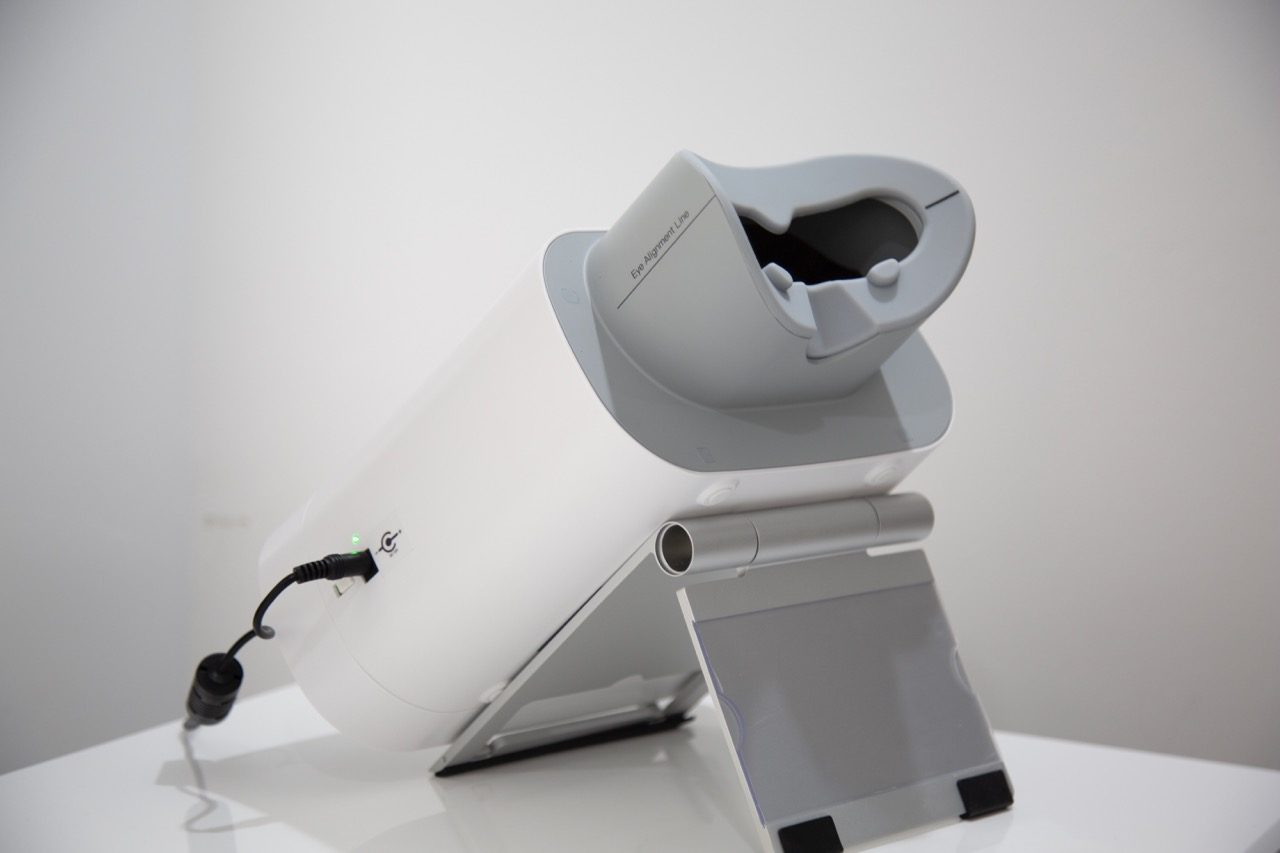
\includegraphics[keepaspectratio]{_resources/images/camera/OpticareCamera1.jpeg}}

}

\caption{Opticare AI眼底相机}

\end{figure}%

\section{初始设置}\label{ux521dux59cbux8bbeux7f6e}

\subsection{设备要求}\label{ux8bbeux5907ux8981ux6c42}

\begin{itemize}
\tightlist
\item
  稳定的桌子或推车
\item
  电源插座
\item
  可靠的互联网连接
\item
  (可选)运行Windows 10或更高版本的计算机或平板电脑
\item
  USB电缆(提供)
\item
  电源适配器(提供)
\end{itemize}

请按照以下步骤开始:

\begin{enumerate}
\def\labelenumi{\arabic{enumi}.}
\item
  \textbf{拆箱相机}:打开箱子,取出相机和支架。
\item
  \textbf{设置支架}:展开支架。确保QR码面向前方。如果您选择不让用户自行扫描,可以取出QR码。
\end{enumerate}

\begin{figure}[H]

{\centering \pandocbounded{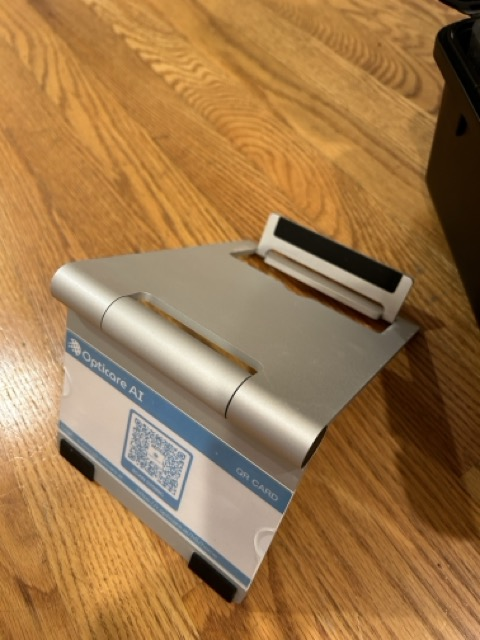
\includegraphics[keepaspectratio]{_resources/images/camera/CameraStand.jpeg}}

}

\caption{将支架设置好,QR码面向前方}

\end{figure}%

\begin{enumerate}
\def\labelenumi{\arabic{enumi}.}
\setcounter{enumi}{2}
\tightlist
\item
  \textbf{移除钥匙}:相机在运输时被锁定。通过移除位于设备底部的螺丝钥匙解锁。
\end{enumerate}

\begin{figure}[H]

{\centering \pandocbounded{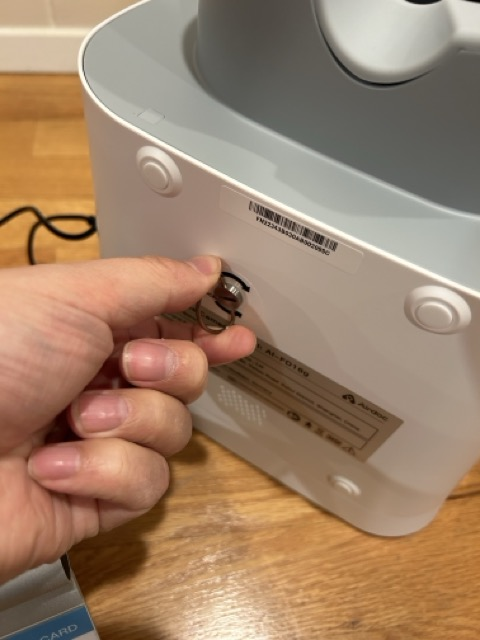
\includegraphics[keepaspectratio]{_resources/images/camera/CameraUnscrew.jpeg}}

}

\caption{逆时针旋转钥匙以移除}

\end{figure}%

\begin{tcolorbox}[enhanced jigsaw, coltitle=black, rightrule=.15mm, colback=white, colbacktitle=quarto-callout-important-color!10!white, breakable, bottomtitle=1mm, opacityback=0, bottomrule=.15mm, titlerule=0mm, opacitybacktitle=0.6, left=2mm, colframe=quarto-callout-important-color-frame, title=\textcolor{quarto-callout-important-color}{\faExclamation}\hspace{0.5em}{保存钥匙!}, toptitle=1mm, toprule=.15mm, arc=.35mm, leftrule=.75mm]

您在打包相机进行运输时将需要这把钥匙,因此请将其放在不会丢失的地方。

\end{tcolorbox}

\textbf{电源连接}:连接电源适配器并打开位于相机左侧的电源开关。绿色指示灯应亮起。

\begin{figure}[H]

{\centering \pandocbounded{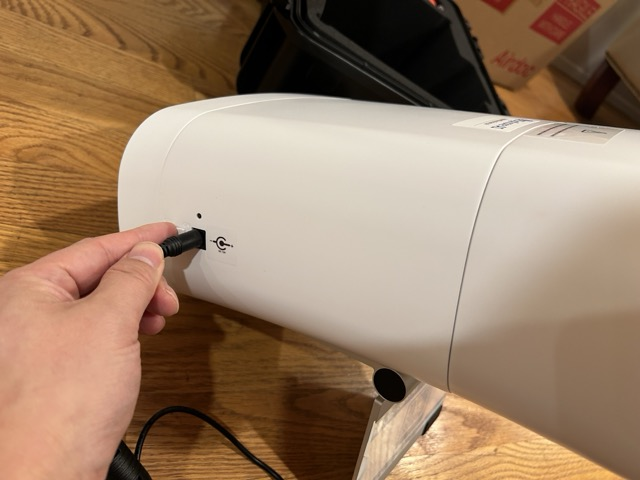
\includegraphics[keepaspectratio]{_resources/images/camera/CameraPowerOn.jpeg}}

}

\caption{将电源连接器连接到相机侧面}

\end{figure}%

\textbf{初始化}:等待相机初始化并提示您进行下一步操作。

\begin{tcolorbox}[enhanced jigsaw, coltitle=black, rightrule=.15mm, colback=white, colbacktitle=quarto-callout-note-color!10!white, breakable, bottomtitle=1mm, opacityback=0, bottomrule=.15mm, titlerule=0mm, opacitybacktitle=0.6, left=2mm, colframe=quarto-callout-note-color-frame, title=\textcolor{quarto-callout-note-color}{\faInfo}\hspace{0.5em}{注记}, toptitle=1mm, toprule=.15mm, arc=.35mm, leftrule=.75mm]

相机已预配置您的Wi-Fi网络。您应该会听到消息:``已连接到网络'',确认它已连接到您的Wi-Fi。请参阅电子邮件以了解设备配置的Wi-Fi信息。

\end{tcolorbox}

\textbf{解锁相机}:快速按下相机右侧较大的白色按钮三次。这将解锁相机。相机下方有一个锁键,需要拧开以解锁。

\subsection{环境优化}\label{ux73afux5883ux4f18ux5316}

\begin{itemize}
\tightlist
\item
  房间照明:适中至昏暗
\item
  温度:保持在5°C - 40°C之间
\item
  湿度:保持在10\% - 90\%之间
\item
  避免设备直射阳光
\item
  确保充足的通风
\end{itemize}

\bookmarksetup{startatroot}

\chapter*{参考文献}\label{ux53c2ux8003ux6587ux732e}
\addcontentsline{toc}{chapter}{参考文献}

\markboth{参考文献}{参考文献}

\phantomsection\label{refs}
\begin{CSLReferences}{1}{0}
\bibitem[\citeproctext]{ref-cheung_retinal_2014}
Cheung, Carol Yim-lui, Yi-Ting Ong, M. Kamran Ikram, Christopher Chen,
和 Tien Yin Wong. 2014. {《Retinal {Microvasculature} in {Alzheimer}'s
{Disease}》}. 编辑 Jack C. De La Torre. \emph{Journal of Alzheimer's
Disease} 42 (s4): S339--52. \url{https://doi.org/10.3233/JAD-141596}.

\bibitem[\citeproctext]{ref-chua_ambient_2020}
Chua, Sharon Y. L., Anthony P. Khawaja, Andrew D. Dick, James Morgan,
Baljean Dhillon, Andrew J. Lotery, Nicholas G. Strouthidis, 等. 2020.
{《Ambient {Air} {Pollution} {Associations} with {Retinal} {Morphology}
in the {UK} {Biobank}》}. \emph{Investigative Opthalmology \& Visual
Science} 61 (5): 32. \url{https://doi.org/10.1167/iovs.61.5.32}.

\bibitem[\citeproctext]{ref-hua_development_2022}
Hua, Rong, Jianhao Xiong, Gail Li, Yidan Zhu, Zongyuan Ge, Yanjun Ma,
Meng Fu, 等. 2022. {《Development and validation of a deep learning
algorithm based on fundus photographs for estimating the {CAIDE}
dementia risk score》}. \emph{Age and Ageing} 51 (12): afac282.
\url{https://doi.org/10.1093/ageing/afac282}.

\bibitem[\citeproctext]{ref-kivipelto_risk_2006}
Kivipelto, Miia, Tiia Ngandu, Tiina Laatikainen, Bengt Winblad, Hilkka
Soininen, 和 Jaakko Tuomilehto. 2006. {《Risk score for the prediction
of dementia risk in 20 years among middle aged people: a longitudinal,
population-based study》}. \emph{The Lancet Neurology} 5 (9): 735--41.
\url{https://doi.org/10.1016/S1474-4422(06)70537-3}.

\bibitem[\citeproctext]{ref-lin_application_2021}
Lin, Duoru, Jianhao Xiong, Congxin Liu, Lanqin Zhao, Zhongwen Li,
Shanshan Yu, Xiaohang Wu, 等. 2021. {《Application of {Comprehensive}
{Artificial} intelligence {Retinal} {Expert} ({CARE}) system: a national
real-world evidence study》}. \emph{The Lancet Digital Health} 3 (8):
e486--95. \url{https://doi.org/10.1016/S2589-7500(21)00086-8}.

\bibitem[\citeproctext]{ref-ma_deep_2022}
Ma, Yanjun, Jianhao Xiong, Yidan Zhu, Zongyuan Ge, Rong Hua, Meng Fu,
Chenglong Li, 等. 2022. {《Deep learning algorithm using fundus
photographs for 10-year risk assessment of ischemic cardiovascular
diseases in {China}》}. \emph{Science Bulletin} 67 (1): 17--20.
\url{https://doi.org/10.1016/j.scib.2021.08.016}.

\bibitem[\citeproctext]{ref-milea_artificial_2020}
Milea, Dan, Raymond P. Najjar, Zhubo Jiang, Daniel Ting, Caroline
Vasseneix, Xinxing Xu, Masoud Aghsaei Fard, 等. 2020. {《Artificial
{Intelligence} to {Detect} {Papilledema} from {Ocular} {Fundus}
{Photographs}》}. \emph{New England Journal of Medicine} 382 (18):
1687--95. \url{https://doi.org/10.1056/NEJMoa1917130}.

\bibitem[\citeproctext]{ref-mitani_detection_2019}
Mitani, Akinori, Abigail Huang, Subhashini Venugopalan, Greg S. Corrado,
Lily Peng, Dale R. Webster, Naama Hammel, Yun Liu, 和 Avinash V.
Varadarajan. 2019. {《Detection of anaemia from retinal fundus images
via deeplearning》}. \emph{Nature Biomedical Engineering} 4 (1): 18--27.
\url{https://doi.org/10.1038/s41551-019-0487-z}.

\bibitem[\citeproctext]{ref-nusinovici_application_2024}
Nusinovici, Simon, Tyler Hyungtaek Rim, Hengtong Li, Marco Yu, Mihir
Deshmukh, Ten Cheer Quek, Geunyoung Lee, 等. 2024. {《Application of a
deep-learning marker for morbidity and mortality prediction derived from
retinal photographs: a cohort development and validation study》}.
\emph{The Lancet Healthy Longevity}, 九月, 100593.
\url{https://doi.org/10.1016/S2666-7568(24)00089-8}.

\bibitem[\citeproctext]{ref-nusinovici_retinal_2022}
Nusinovici, Simon, Tyler Hyungtaek Rim, Marco Yu, Geunyoung Lee,
Yih-Chung Tham, Ning Cheung, Crystal Chun Yuen Chong, 等. 2022.
{《Retinal photograph-based deep learning predicts biological age, and
stratifies morbidity and mortality risk》}. \emph{Age and Ageing} 51
(4): afac065. \url{https://doi.org/10.1093/ageing/afac065}.

\bibitem[\citeproctext]{ref-tsukahara_is_2021}
Tsukahara, Jason S., 和 Randall W. Engle. 2021. {《Is baseline pupil
size related to cognitive ability? {Yes} (under proper lighting
conditions)》}. \emph{Cognition} 211 (六月): 104643.
\url{https://doi.org/10.1016/j.cognition.2021.104643}.

\bibitem[\citeproctext]{ref-wong_retinal_2002}
Wong, Tien Yin. 2002. {《Retinal {Arteriolar} {Narrowing} and {Risk} of
{Diabetes} {Mellitus} in {Middle}-aged {Persons}》}. \emph{JAMA} 287
(19): 2528. \url{https://doi.org/10.1001/jama.287.19.2528}.

\bibitem[\citeproctext]{ref-xia_generalizing_2024}
Xia, Peng, Ming Hu, Feilong Tang, Wenxue Li, Wenhao Zheng, Lie Ju, Peibo
Duan, Huaxiu Yao, 和 Zongyuan Ge. 2024. {《Generalizing to {Unseen}
{Domains} in {Diabetic} {Retinopathy} with {Disentangled}
{Representations}》}. arXiv. \url{http://arxiv.org/abs/2406.06384}.

\bibitem[\citeproctext]{ref-zhao_foundation_2024}
Zhao, Theodore, Yu Gu, Jianwei Yang, Naoto Usuyama, Ho Hin Lee, Sid
Kiblawi, Tristan Naumann, 等. 2024. {《A foundation model for joint
segmentation, detection and recognition of biomedical objects across
nine modalities》}. \emph{Nature Methods}, 十一月.
\url{https://doi.org/10.1038/s41592-024-02499-w}.

\bibitem[\citeproctext]{ref-zhu_retinal_2023}
Zhu, Zhuoting, Danli Shi, Peng Guankai, Zachary Tan, Xianwen Shang,
Wenyi Hu, Huan Liao, 等. 2023. {《Retinal age gap as a predictive
biomarker for mortality risk》}. \emph{British Journal of Ophthalmology}
107 (4): 547--54.
\url{https://doi.org/10.1136/bjophthalmol-2021-319807}.

\end{CSLReferences}


\backmatter


\end{document}
